\documentclass[12pt]{article}
\usepackage{amssymb,amsmath,pgf,setspace,comment,multicol,verbatim,titling,pdflscape}
\usepackage[labelfont=bf]{caption}
\usepackage[left=1in,right=1in,top=1in,bottom=0.75in]{geometry}
\usepackage[round]{natbib}
\doublespacing

\setlength{\droptitle}{-50pt}

%% Auto-generated by O3-paper-numbers.do — do not edit by hand
\newcommand{\nPCPs}{51,067}
\newcommand{\nSpecialists}{9,254}
\newcommand{\meanRefsPerPCP}{4.40}
\newcommand{\meanSpecsPerPCP}{3.11}
\newcommand{\meanRefsPerPair}{1.41}
\newcommand{\meanRefsPerSpec}{30.04}
\newcommand{\meanFailuresPerPCP}{0.40}
\newcommand{\failureRateMean}{9}
\newcommand{\specFailurePtwentyfive}{6.52}
\newcommand{\specFailurePseventyfive}{13.04}
\newcommand{\failureIQRPtwentyfive}{4.49}
\newcommand{\failureIQRMedian}{5.05}
\newcommand{\failureIQRPseventyfive}{5.70}
\newcommand{\paymentIQRMedian}{8}
\newcommand{\capacitySuffPct}{39}
\newcommand{\meanChoiceSet}{57}
\newcommand{\meanSpecsPerHRR}{83}
\newcommand{\runningReferrals}{4.44}
\newcommand{\specsPerHRRYear}{69}
\newcommand{\cumlNetworkSize}{10}
\newcommand{\nHRRsMNL}{291}
\newcommand{\specPatientsMeanSixYr}{127.87}
\newcommand{\specPatientsSdSixYr}{163.18}
\newcommand{\specPatientsMeanHone}{74.00}
\newcommand{\specPatientsSdHone}{86.12}
\newcommand{\specPatientsMeanHtwo}{74.70}
\newcommand{\specPatientsSdHtwo}{87.03}
\newcommand{\topSpecShare}{0.33}
\newcommand{\condRefProb}{0.10}

%% Auto-generated by O2-structural-summary.do — do not edit by hand
\newcommand{\reallocationMeanMyopic}{39.6}
\newcommand{\healthFXMeanMyopic}{0.5}
\newcommand{\nHRRsMyopic}{280}
\newcommand{\nAlphaZeroMyopic}{51}
\newcommand{\alphaDistRatioMyopic}{2.9}
\newcommand{\nHRRsEtaFiveMyopic}{281}
\newcommand{\reallocationMeanFullFamMyopic}{40.0}
\newcommand{\healthFXMeanFullFamMyopic}{0.4}
\newcommand{\partialFXNonzeroMyopic}{3.4}
\newcommand{\partialFXAllMyopic}{2.5}
\newcommand{\reallocationMeanFWD}{32.1}
\newcommand{\healthFXMeanFWD}{0.4}
\newcommand{\nHRRsFWD}{277}
\newcommand{\nAlphaZeroFWD}{46}
\newcommand{\alphaDistRatioFWD}{3.8}
\newcommand{\nHRRsEtaFiveFWD}{279}
\newcommand{\reallocationMeanFullFamFWD}{35.0}
\newcommand{\healthFXMeanFullFamFWD}{0.4}
\newcommand{\partialFXNonzeroFWD}{3.0}
\newcommand{\partialFXAllFWD}{2.0}


\begin{document}

\title{Learning and the Efficiency of Physician Referrals \\
SUPPLEMENTAL APPENDIX}
\author{%
  Ian M. McCarthy \\[-1.5ex]
  Emory University \& NBER \\
  Seth Richards-Shubik \\[-1.5ex]
  Johns Hopkins University \& NBER
}
\date{July 2026}
\maketitle


%%% A. DATA AND DESCRIPTIVE STATISTICS
\section{Data and Descriptive Statistics}
\label{app:desc}

This section provides additional details of our analytic data and subsequent referral patterns.

\subsection{PCP Identification}
\label{app:pcp-validation}

Our method identifies a patient's PCP using a carrier-claims lookback window, selecting the most-visited PCP in pre-surgery E\&M claims. Table \ref{tab:pcp-validation} compares this approach with the referring physician listed on the surgeon's claim (\texttt{rfr\_physn\_npi}). The listed referring physician field is not populated in roughly 32\% of cases, and when it is populated, it most often lists the surgeon (self-referral, about 43\%) or a non-PCP specialist (about 7\%). Only about 18\% of cases list a PCP as the referring physician. Among cases where both methods identify a PCP, concordance exceeds 82\% in every year.

Figure \ref{fig:pcp-validation} shows the composition of the listed referring physician field alongside our lookback coverage rate. Our lookback method identifies a PCP for approximately 80\% of procedures, providing substantially better coverage than the listed field alone.


%%% B. REDUCED-FORM EVIDENCE

\section{Reduced-Form Evidence}
\label{app:reduced-form}

The main paper reports stacked event-study estimates combining all four failure cohorts. Figure \ref{fig:event-cohort} presents the cohort-specific estimates separately for first, second, third, and fourth failures. The patterns are consistent with the stacked results. Each cohort shows a significant and persistent reduction in referrals from the treated PCP following the failure event, with flat pre-trends and no convergence within the observed nine-quarter window. The magnitudes are somewhat larger for the first and second failure cohorts than for the third and fourth, consistent with attenuating responses as PCPs have already adjusted expectations after earlier signals.


%%% C. IDENTIFICATION

\section{Identification} \label{app:identification}

We formally show identification of the myopic model below. Identification of the forward-looking model, discussed in the main paper, follows because the Brezzi-Lobo approximation to the Gittins index involves the same free parameters ($\rho$ and $\eta$) on the same data as the myopic mean belief, and the present discounted value of familiarity has a known relationship with its current value. The forward-looking model therefore introduces no additional free parameters beyond those of the myopic model.


\subsection{Myopic Model}

We start by proving the identification of the myopic model.
To review (and simplify), the utility to PCP $i$ for referring patient $t$ to specialist $j$ is
\[
U_{ijt} \equiv \alpha m_{ijt} + f(e_{ijt}) + \xi_j + \epsilon_{ijt},
\]
where $m_{ijt}$ is the current mean of the beliefs about the probability of success at specialist $j$ (using the history before patient $t$), $e_{ijt}$ is the amount of experience with specialist $j$ (the number of past patients $i$ sent to $j$), $f(e_{ijt})$ is the subjective utility from familiarity with specialist $j$, $\xi_j$ is an unobservable specialist fixed effect, and $\epsilon_{ijt}$ is an idiosyncratic shock with a known distribution.
Also let $\check y_{ijt}$ denote the number of successes among past patients that $i$ sent to $j$.
% NOTE: There is no outside option with utility normalized to zero.

Given a parametric assumption on the error term, $\epsilon$, the observable choice probabilities directly identify differences in utility, excluding the error term: e.g., $(U_{ijt} - \epsilon_{ijt}) - (U_{ikt} - \epsilon_{ikt})$.
To simplify these expressions, let $v$ denote utility without the error term: $v \equiv U - \epsilon$.

To be somewhat more precise, there is a finite number of specialists but large numbers of patients and PCPs.
The choice probabilities are
\[
\Pr(j | (e_{ikt}, \check y_{ikt})_{k=1}^J) ,
\]
where ``$j$'' means the event that specialist $j$ is chosen.
We may need consistent estimates of the choice probabilities for cases where $e_{ikt} = 0, \forall k$, and where $e_{ikt} \to \infty, \forall k$.
Hence the number of PCPs may need to go to infinity, but the number of patients must grow faster.


%The effects of the exogenous characteristics, $u(x)$, follow from separate variation in $x$, as is standard.
%The effect of congestion, $c(n_{jt})$ is identified from separate variation in $n_{jt}$, which requires a valid instrument for the endogenous patient volume, described elsewhere.
We identify the remaining components of $v$ in steps as follows.
\begin{enumerate}
    \item Specialist fixed effects ($\xi$):
Any cases where the observables are the same for two specialists can be used to identify the fixed effects (up to a standard normalization; e.g., one fixed effect is set to zero).
Because if $e, \check y, x, n$ are the same, then
$$ v_{ijt} - v_{ikt} = \xi_j - \xi_k . $$
In particular, cases where $e=0$ (and hence $\check y = 0$) are useful here.
    \item Altruism parameter ($\alpha$):
This uses cases with large past experience, formally the limit when $e \rightarrow \infty$.
Let $e_{ijt} \rightarrow \infty$ and $e_{ikt} \rightarrow \infty$
(and for convenience $x_{ijt} = x_{ikt}$ and $n_j = n_k$).
Then
\[ v_{ijt} - v_{ikt} 
= \frac{ \alpha \bar y_{ijt} }{ 0 + 1 } + \xi_j
- \frac{ \alpha \bar y_{ikt} }{ 0 + 1 } - \xi_k .
\]
% [I CAN PULL UP MORE OF THE ALGEBRA FROM BELOW.]
Hence
\[ \alpha 
= \frac{(v_{ijt} - \xi_j) - (v_{ikt} - \xi_k)}
  {\bar y_{ijt} - \bar y_{ikt}}
\]
in these limits.
Thus cases where a PCP has large past experience with two specialists, but different success rates with them, identify the altruism parameter.
    \item Strength of priors ($a_0 + b_0$):
The responsiveness to success with finite experience then identifies the strength of priors (i.e., the stickiness of beliefs).
Let $e_{ijt} = e_{ikt} = e$
(and for convenience $x_{ijt} = x_{ikt}$ and $n_j = n_k$).
Then
\[ v_{ijt} - v_{ikt} 
= \frac{ \alpha \check y_{ijt}}{ a_0 + b_0 + e } + \xi_j
- \frac{ \alpha \check y_{ikt}}{ a_0 + b_0 + e } - \xi_k .
\]
Hence
\[ (a_0 + b_0) 
= \frac{\alpha (\check y_{ijt} - \check y_{ikt})}
{(v_{ijt} - \xi_j) - (v_{ikt} - \xi_k)} - e ,
\]
and all the objects on the right are observable or already identified.
    \item Effect of familiarity ($f(e)$):
Finally, differences in experience with specialists identify the effect of familiarity.
For convenience let $x, n$ be the same, then
\[ v_{ijt} - v_{ikt} 
= \alpha \frac{a_0 + \check y_{ijt}}{ a_0 + b_0 + e_{ijt} } + f(e_{ijt}) + \xi_j
- \alpha \frac{a_0 + \check y_{ikt}}{ a_0 + b_0 + e_{ikt} } - f(e_{ikt}) - \xi_k .
\]
Hence
\begin{align*}
 f(e_{ijt}) - f(e_{ikt}) 
\ = \  & (v_{ijt} - \xi_j) - (v_{ikt} - \xi_k) \\
& - \alpha \left[ \frac{a_0}{ a_0 + b_0 + e_{ijt} } - \frac{a_0}{ a_0 + b_0 + e_{ikt} } \right] \\
& - \alpha \left[ \frac{\check y_{ijt}}{ a_0 + b_0 + e_{ijt} } - \frac{\check y_{ikt}}{ a_0 + b_0 + e_{ikt} } \right] .
\end{align*}
This identifies $f$ up to a normalization, specifically $f(0) = 0$.

However this also requires the value of $a_0$, which can be obtained if the prior ratio, $\frac{a_0}{a_0 + b_0}$, is calibrated separately.
Intuitively, we need to fully identify the priors (both the ratio and the strength) in order to recover the effect of familiarity, because we need to know exactly how experience washes away the priors in order to separate that from the effect of familiarity.
\end{enumerate}

%%%

\subsection{Monte Carlo Evidence on the Recovery of $\alpha$}
\label{app:monte-carlo}

% TODO (Seth): I have no memory of this... Can we cut it?
% IAN: I added all of this. We can definitely cut it if you want. Seemed useful to me but no biggie.

To assess the finite-sample properties of our estimator, we conduct a Monte Carlo simulation calibrated to match key features of our data. We generate referral markets with 50 PCPs and 10 specialists, where each PCP makes 15 referrals per year. We include a burn-in period to establish referral histories and rely on a 6-year estimation window to match the estimation in our real data. Specialists are assigned heterogeneous quality levels (true failure probabilities) drawn from a normal distribution centered at the base failure rate, and each specialist receives a fixed effect drawn independently. PCPs choose specialists according to the myopic structural model presented in the main text, with beliefs updated via Bayes' rule after each patient outcome.

We estimate $\hat\alpha$ using the same constrained maximum likelihood procedure used in the main estimation (see Section \ref{app:estimation}), with specialist fixed effects included in the multinomial logit. We vary the true $\alpha$ over the range 0.05 to 0.60, the base failure rate over 0.05 to 0.15, and the quality dispersion (standard deviation of failure rates across specialists) over 0.01 to 0.05, yielding 77 parameter configurations after excluding cases where the quality dispersion exceeds the base failure rate. For each configuration, we run 50 replications.

Figure \ref{fig:bias-surface} presents the bias in $\hat\alpha$ as a function of the true $\alpha$ and the base failure rate, holding quality dispersion fixed at 0.03 (approximately matching the interquartile range of failure rates in the data). The surface reveals that bias is primarily driven by the magnitude of the true $\alpha$, with a secondary role for the base failure rate. Bias is largest when the true $\alpha$ is small, because the signal from patient outcomes is weak relative to the noise from the logit errors and the specialist fixed effects. Higher base failure rates improve identification by producing more frequent failures, which accelerates belief updating.

Figure \ref{fig:relbias-alpha} presents the relative bias (as a percentage of the true $\alpha$) for each failure rate, again at quality dispersion of 0.03. Relative bias falls below 10\% for $\hat\alpha \geq 0.30$ when the base failure rate is 0.09 or higher. Among markets with non-zero estimates of $\hat\alpha$, the mean is 0.25 for $\eta = 1$ and 0.43 for $\eta = 5$ in the myopic model (0.32 and 0.54 in the forward-looking model), with the 75th percentile at 0.32 and above in all cases. The overwhelming majority of markets therefore either suggest very little learning ($\hat\alpha = 0$) or fall in the range where the estimator appears to perform well. These simulation results also support our decision to fix $\eta$ rather than estimate it jointly with $\alpha$, as the likelihood surface with respect to $\eta$ is relatively flat across the parameter configurations we examined.


\subsection{Simulation study on identification of $\eta$}

Although we have shown that $\eta$ is identified, our preliminary estimates of this parameter exhibited poor performance and so we used fixed values instead. Here we present a simulation study that indicates the data in our application would indeed have little power to inform an estimate of $\eta$.

We simulate a market with 2,500 patients and 25 specialists. For simplicity, the PCP-specialist histories (\# referrals, \# successes) are independent across patients, as though each patient were treated by a different PCP, but the PCPs have prior histories with some specialists. Each PCP has a 0.2 probability of any history with each specialist, independent across specialists. Conditional on any history with a specialist, the number of past referrals is Poisson with mean 4, and the number of past successes is binomial using the number of past referrals and the surgeon's success probability (explained below).

The simulation model has the same specification as our empirical model, except that there is no congestion effect and the familiarity effect is specified as $f(e_{ijt}) = \beta \ln(1+e_{ijt})$. The parameter values are as follows:
\begin{itemize} \singlespacing
    \item $\alpha = 0.3$ (weight on outcome)
    \item $\pi = -0.07$ (weight on distance)
    \item $\beta = 0.9$ (weight on familiarity)
    \item $\eta = 3$ (prior strength)
    \item $\rho$: explained below (prior mean)
    \item $\xi$: explained below (fixed effects)
\end{itemize}
Specialist qualities, $q_j$, are drawn independently from a normal distribution with mean 0.9 and SD 0.04, and censored symmetrically at 0.81 and 0.99. The prior mean, $\rho$, is set equal to the average of these draws. The specialist fixed effects, $\xi_j$, are given fixed values on a grid from $-1.5$ to $+1.5$ with equal intervals of 3/25 between values.

Figure \ref{fig:eta-simulation} shows the results from four representative simulations. It plots log-likelihood values obtained using a wide range of values for $\eta$ while keeping the other parameters at their true values. It is apparent that the likelihood function is very flat in this parameter. The log likelihood changes by only a few points over the entire span of values for $\eta$. Across 100 such simulations, the average range of the likelihood values is only 2.1 log points and the 95th percentile is 4.3 log points. Based on this, we do not think the data in our application would have good power to yield an informative estimate of $\eta$.




%%% D. ESTIMATION

\section{Estimation}
\label{app:estimation}

\subsection{Iterative Estimation of $\alpha$}
\label{app:fader}

To constrain $\alpha \geq 0$ we estimate $\ln \alpha$ and specify the beliefs term as $\exp(\ln \alpha) \cdot m$ (or $\exp(\ln \alpha) \cdot g(m,v)$ in the forward-looking model).
We use an iterative procedure proposed in \cite{fader1992} which makes it possible to employ standard estimation commands designed for multinomial logits where all terms are linear in parameters.
The procedure is based on a first-order Taylor series approximation of the term that is nonlinear in parameters.
With the exponential function this is simply
$$ \exp(\ln \alpha_2) \cdot m \approx \left[ \exp(\ln \alpha_1) + (\ln \alpha_2 - \ln \alpha_1) \exp(\ln \alpha_1) \right] \cdot m,$$
(because $d \exp(\ln \alpha) / d \ln \alpha = \exp(\ln \alpha)$), where $\ln \alpha_1$ and $\ln \alpha_2$ are two candidate values.

In our case, the iteration works by setting a value of $\ln \alpha$ (e.g., $\ln \alpha_1$) and then estimating the model with a free coefficient (e.g., $\hat \pi_1$) on the term $\exp(\ln \alpha_1) \cdot m$.  Rearranging the Taylor approximation above shows how the estimated coefficient can be used to update the value of $\ln \alpha$, as follows:
\[
     \exp(\ln \alpha_2) \cdot m \approx \underbrace{[1 + (\ln \alpha_2 - \ln \alpha_1)]}_{\hat \pi_1} \exp(\ln \alpha_1) \cdot m ;
\]
hence:
\[
    \ln \alpha_2 = \ln \alpha_1 + \hat \pi_1 - 1 .
\]
Furthermore, because the estimated coefficient $\hat \pi_1$ by definition improves the likelihood, using $\exp(\ln \alpha_2)$ should produce a higher likelihood than $\exp(\ln \alpha_1)$.
\cite{fader1992} prove that this algorithm converges to the MLE of $\ln \alpha$ under standard regularity conditions.
For some intuition note that at the maximum, $\ln \alpha_*$, the likelihood cannot be improved, and so the value of $\hat \pi$ should be one; i.e., in terms of the Taylor expansion
\[
    \exp(\ln \alpha_*)
    = \underbrace{[1 + (\ln \alpha_* - \ln \alpha_*)]}_{\hat \pi_*} \exp(\ln \alpha_*)
    = \underbrace{[1]}_{\hat \pi_*} \exp(\ln \alpha_*)
\] 
The standard error then follows from \cite{fader1992} as
\[
    SE(\hat \alpha) = \exp(\ln \alpha_*) SE(\hat \pi_*)
\]
because $\hat \alpha = \exp(\ln \alpha_*) = \exp(\ln \alpha_* + \hat \pi_* - 1)$ and asymptotically we only need to consider the variation in $\hat \pi_*$ (see Lemma 2 in \citealp{fader1992}).

%%%


%%% First Stage Diagnostics

\subsection{First-Stage Diagnostics for Congestion}
\label{app:first-stage}

Specialist patient volume, $n_{jt}$, is endogenous in the referral utility because unobserved specialist characteristics that raise utility (and therefore referrals) would mechanically raise volume. To separate the causal effect of congestion on referral appeal from this correlation, we instrument for $n_{jt}$ using a distance-based predicted patient count, following \citet{richards-shubik2021}. For each specialist and time period, the instrument is a distance-predicted patient count, constructed by estimating a conditional logit of referral choice with patient-to-surgeon distance as the sole covariate, then summing the predicted choice probabilities across patients for each specialist. The instrument varies across specialists through the geographic distribution of PCPs and patients, and it is independent of specialists' unobserved quality or taste shifters conditional on the HRR fixed effects that absorb market-wide demand. The exclusion restriction is standard in the spatial choice literature: conditional on HRR, the geographic configuration of PCPs relative to specialists affects referrals only through the distance channel, not directly through quality.

The first stage regresses specialist total patients on the distance-based instrument, HRR fixed effects, and a time-period indicator, weighted by the inverse variance of the specialist fixed effect estimate and clustered at the specialist level. Table \ref{tab:first-stage} reports the pooled results. The first-stage coefficient is close to one and precisely estimated, indicating that a one-patient increase in the distance-predicted count corresponds to roughly a one-patient increase in realized volume after absorbing market-level differences. The F-statistic on the excluded instrument exceeds one thousand in both specifications, well above conventional thresholds for weak-instrument concerns \citep{stock2005}. The estimates are nearly identical across $\eta = 1$ and $\eta = 5$ because the instrument and the endogenous variable do not depend on the learning model.

Figure \ref{fig:fs-scatter} presents partial scatter plots after residualizing both the instrument and patient volume on HRR fixed effects and the time-period indicator. The relationship is visibly linear across the range of the residualized instrument, with no evidence of influential observations driving the pooled coefficient. Weighting by the inverse variance of the specialist fixed effect gives more influence to specialists with more precisely estimated effects, which also tend to be higher-volume specialists for whom the congestion mechanism is most empirically relevant.

A pooled first stage averages across HRRs of different sizes, so we also estimate the first stage separately in each HRR. Figure \ref{fig:fs-fstat} shows the distribution of HRR-level F-statistics, weighted by the number of patients in each HRR so that larger markets (where most identification comes from) receive more weight. The distribution is concentrated well above the conventional $F = 10$ threshold, with the large majority of patients in markets that comfortably satisfy the weak-instrument diagnostic. A minority of smaller HRRs exhibit low F-statistics, reflecting the small number of specialists and the limited spatial variation within those markets rather than a systematic failure of the instrument. Because our structural estimation pools information across HRRs through the common $\gamma$, the strength of the pooled first stage is the relevant benchmark for inference on congestion.


%%% Model Fit Diagnostics

\subsection{Model Fit Diagnostics}
\label{app:fit}

We examine two diagnostics that together assess model fit and defend the structural interpretation of the parameters. Figure \ref{fig:fit-shares} plots predicted versus actual referral shares at the specialist level, which is a standard validation for discrete-choice models. The predicted shares track actual shares closely across the range, with no systematic bias at the high or low end.

Figure \ref{fig:fe-quality} addresses a different concern. If the specialist fixed effects, $\xi_j$, were simply absorbing quality differences that our measure does not capture, then the estimated $\alpha$ would be biased toward zero and the reported counterfactuals would understate the gains from information. The figure shows that the within-HRR correlation between estimated $\xi_j$ and observed specialist quality is near zero in most markets. The fixed effects therefore capture demand factors that are empirically distinct from outcome-based quality, supporting the interpretation of $\alpha$ as a separate learning channel.


%%% Sensitivity of alpha

\subsection{Sensitivity of the Quality Response to Alternative Specifications}
\label{app:alpha-sensitivity}

Re-estimating the structural model and recomputing counterfactuals for every alternative specification is computationally prohibitive. As a more tractable diagnostic, we examine how the estimated quality response, $\alpha$, varies across alternative specifications of the choice model, estimated separately within each HRR. In the myopic case, the choice model is
\begin{equation}
 \text{E}\left[ U_{ijt} \mid \dots \right] = \alpha\, m_{ijt} + \pi x_{ijt} + \sum_{b \in B} \kappa_b\, I(e_{ijt} \in b) + \delta_j + \epsilon_{ijt} ,
\label{eqn:choice-mnl}
\end{equation}
where $m_{ijt}$ is the posterior mean belief about specialist $j$'s quality and $\delta_j$ is a single, time-invariant specialist fixed effect. This matches the myopic specification in the main text, except that the composite time-varying effect $\delta_{j,\tau(t)} = \gamma n_{j,\tau(t)} + \xi_j$ is replaced by one fixed effect $\delta_j$ per surgeon, which lets the diagnostic run quickly across the full set of HRRs. We estimate $\alpha$ with the same iterative procedure used for the structural model, which constrains $\alpha \geq 0$. Because the counterfactual reallocations and health effects scale directly with $\alpha$ in each market, stability of $\alpha$ across specifications implies stability of our counterfactual conclusions.

Table~\ref{tab:coefficients} reports the distribution of $\hat\alpha$ across HRRs under three specifications. The ``Baseline'' specification matches the main-text estimates. The ``Integrated'' specification adds an indicator for the PCP and specialist sharing a practice. The ``Peer Outcomes'' specification further includes a measure of specialist quality constructed from the outcomes of other PCPs' patients in the same practice. All three impose time-invariant congestion for computational ease. The mean $\hat\alpha$ moves from 0.192 in the baseline to 0.192 with the practice indicator and 0.203 with the peer-quality measure, and the upper-tail percentiles are similarly stable. The estimated quality response is therefore not driven by failing to control for practice integration or peer-based quality information.

\subsection{Risk Adjustment}
\label{app:risk-adjustment}

Here, we discuss how risk adjustment does not materially affect our estimates of specialist quality. First, our sample is heavily concentrated in a single, low-complexity DRG. Table~\ref{tab:drg-distribution} reports the distribution of admissions across DRGs. DRG 470 (major joint replacement of lower extremity, without MCC) accounts for 86.1 percent of the 2.9 million events, with the remaining 14 percent spread across 17 procedure codes. The combination of elective admission and physician referral as sample inclusion criteria selects a planned, lower-complication population in which case-mix variation across specialists is limited. Indeed, consistent with this homogeneity, the Comprehensive Care for Joint Replacement model similarly incorporated limited additional patient-level risk adjustment in setting its bundled payment amounts \citep{ccjr-lewin-2021}.

Second, raw and risk-adjusted specialist quality are highly correlated. We construct a risk-adjusted quality measure by regressing the patient-level 90-day failure indicator on age (quadratic), sex, race, DRG, and the Charlson Comorbidity Index, then taking each specialist's observed minus expected failure rate plus the overall sample mean. The Pearson correlation between the raw and risk-adjusted measures is 0.84, so adjusting for observable patient case-mix moves the cross-section of specialist quality very little on average.

Third, the estimated quality response is invariant to either case-mix sensitivity. Table~\ref{tab:coefficients-adj} reports the distribution of $\hat\alpha$ under two re-estimations of the choice model in Equation~\eqref{eqn:choice-mnl}. The first restricts the estimation sample to DRG 470 only, and the second swaps the risk-adjusted specialist-quality measure into the belief prior. The mean of $\hat\alpha$ moves from 0.192 in the baseline (Table~\ref{tab:coefficients}) to 0.216 when restricting to DRG 470 only, and to 0.192 with the risk-adjusted quality measure. The upper-tail percentiles are similarly stable.

Because the sample is concentrated in a single elective DRG, the raw and risk-adjusted quality measures are tightly correlated, and the estimated quality response is invariant to either case-mix sensitivity, we retain the raw specialist-quality measure throughout. Even setting these results aside, the structural model would not easily accommodate a continuous risk-adjusted signal. The beta-binomial belief-updating framework presumes binary outcomes, and the path to a comparable model that admits continuous signals (e.g., normal-normal updating with a corresponding Gittins index) is unclear.


%%% E. COUNTERFACTUAL ROBUSTNESS

\section{Counterfactual Robustness}
\label{app:cf-robustness}

\subsection{Counterfactuals without Familiarity}
\label{app:cf-fullfam}

The purpose of this counterfactual is to estimate the potential changes in referrals and subsequently patient health if PCPs could rely entirely on specialist quality, with full information, and without any attachment due to prior relationships. These results are presented in Figure \ref{fig:cf_fullfam}. Here, we estimate larger effects on referral probabilities, with reallocation of \reallocationMeanFullFamMyopic{} percent on average across HRRs. However, the health effects of this scenario are negative on average, with a change in success rates of \healthFXMeanFullFamMyopic{} percentage points. Without any familiarity to anchor referral patterns, and with the estimated weight on quality small relative to distance preferences and specialist fixed effects, the reallocation proceeds largely independently of quality. This result reinforces the finding in the main text that existing referral relationships encode quality information, and that removing them eliminates an important source of quality sorting in the referral market.

\subsection{Equilibrium Robustness}
\label{app:robustness}

To confirm the robustness of the counterfactual equilibrium, we re-solve the fixed point from two extreme starting values, zero patients at every specialist and the observed patient volumes, in a stratified sample of six HRRs spanning small, medium, and large markets. Table \ref{tab:robustness} reports the results. Across 1,021 specialist-period observations, the mean absolute difference in specialist shares within an HRR-period is 0.7 to 1.9 percentage points, and roughly three-quarters of specialists agree to within one percentage point across the two starts. At the HRR level, the patient-weighted mean of specialist quality differs by at most $7 \times 10^{-5}$ between the two starting values, roughly an order of magnitude smaller than the counterfactual-induced changes we report. Our counterfactual equilibrium is therefore robust to starting value, and the aggregate outcomes we use in the analysis are effectively invariant.

\subsection{Distributional Effects on Quality}
\label{app:distributional}

In addition to the changes in mean quality reported in the main text, we examine how counterfactual reallocation reshapes the within-HRR distribution of specialist quality. Figures \ref{fig:qualP10-cf} and \ref{fig:qualP90-cf} present off-diagonal scatters of the 10th and 90th patient-weighted percentiles of specialist quality under each counterfactual against the corresponding baseline values. Points falling on the 45-degree line represent HRRs where the percentile is unchanged, which dominates in most markets because weighted percentiles are step functions over a discrete set of specialists and small reallocations do not cross the relevant specialist boundary. The off-diagonal scatters drop these unchanged points to focus attention on HRRs where the distribution actually shifts.

Two patterns emerge. Under the existing-familiarity counterfactual, both the 10th and 90th percentiles of quality shift upward on average in markets where they move, consistent with the distribution compressing toward higher quality and producing the small positive mean quality effect reported in the main text. Under the reset-familiarity counterfactual, the 10th percentile shifts downward while the 90th shifts upward, indicating that resetting familiarity increases dispersion. A minority of patients are reallocated to higher-quality specialists they had previously been far from, while another group loses the quality cues embedded in their prior referral patterns and is reallocated to lower-quality specialists. The net mean effect under the reset-familiarity counterfactual is slightly negative because the losses at the bottom of the distribution outweigh the gains at the top.

\subsection{Distributional Effects on Spending}
\label{app:distributional-spending}

As a diagnostic on the direction of these reallocations, we also examine how the counterfactual shifts the within-HRR distribution of episode spending. Figures \ref{fig:spendP10-cf} and \ref{fig:spendP90-cf} present off-diagonal scatters of the 10th and 90th patient-weighted percentiles of episode spending under each counterfactual. The broad widening pattern of the quality distribution under reset familiarity also appears in spending, with the 10th and 90th percentiles moving in opposite directions in markets where the distribution shifts. Some of this co-movement between spending and quality is mechanical, since surgical complications and readmissions enter both our quality measure and 90-day episode spending.

%%% BIBLIOGRAPHY

\pagebreak
\bibliographystyle{aer}
\bibliography{BibTeX_Library}

%%% TABLES AND FIGURES

\clearpage
\section*{Tables and Figures}

%%% TABLES

\begin{table}[h!]
\centering
\footnotesize
\begin{minipage}[h]{6in}
\caption[PCP Identification Validation]{\textbf{PCP Identification Method Validation}\footnote{Comparison of our carrier-lookback PCP identification method with the referring physician listed on the surgeon's claim (\texttt{rfr\_physn\_npi}). ``Not Pop.'' indicates the referral field is not populated. ``Self-Referral'' indicates the listed referring physician is the operating surgeon. ``Non-PCP'' indicates a non-PCP specialist. ``PCP'' indicates a primary care physician. ``Lookback Coverage'' is the share of procedures for which our method identifies a PCP. ``Concordance'' is the share of cases where both methods identify a PCP and they agree.}}
\centerline{%
\begin{tabular}{lrcccccc}
\hline\hline
 & & \multicolumn{4}{c}{Composition of Referral Field (\%)} & Lookback & \\
\cline{3-6}
Year & Procedures & Not Pop. & Self-Referral & Non-PCP & PCP & Coverage (\%) & Concordance (\%) \\
\hline
2013 & 445,274 & 30.1 & 41.6 & 7.5 & 20.8 & 81.5 & 82.8 \\
2014 & 456,377 & 31.2 & 41.6 & 7.1 & 20.1 & 80.9 & 82.7 \\
2015 & 502,927 & 31.1 & 42.9 & 7.1 & 18.9 & 80.5 & 82.8 \\
2016 & 542,126 & 31.5 & 43.7 & 7.1 & 17.8 & 79.8 & 82.4 \\
2017 & 557,277 & 32.6 & 44.1 & 6.7 & 16.6 & 79.0 & 82.7 \\
2018 & 506,138 & 34.4 & 43.5 & 6.5 & 15.6 & 78.2 & 82.1 \\
\hline
All & 3,010,119 & 31.9 & 43.0 & 7.0 & 18.2 & 79.9 & 82.6 \\
\hline\hline
\end{tabular}

}
\label{tab:pcp-validation}
\end{minipage}
\end{table}

\clearpage
\begin{table}[h!]
\centering
\footnotesize
\begin{minipage}[h]{5in}
\caption[First-Stage Results]{\textbf{First-Stage Results for Congestion 2SLS}\footnote{Pooled first-stage regression of specialist total patients on distance-predicted patient counts, with HRR fixed effects and a time-period indicator. Observations weighted by the inverse variance of the specialist fixed effect estimate. Standard errors clustered at the specialist level. Results shown for the myopic model; the forward-looking model yields nearly identical first-stage estimates because the instrument and endogenous variable do not depend on the learning model.}}
\centerline{%
\begin{tabular}{lcccc}

& Coefficient & SE & F-statistic & N \\
\hline\hline
$\eta=1$ & 1.418 & (0.040) & 1236.5 & 36,509 \\
$\eta=5$ & 1.415 & (0.041) & 1171.9 & 36,543 \\
\hline

\end{tabular}
}
\label{tab:first-stage}
\end{minipage}
\end{table}

\clearpage
\begin{table}[h!]
\centering
\footnotesize
\begin{minipage}[h]{6in}
\caption[Sensitivity Analysis]{\textbf{Sensitivity Analysis}\footnote{Estimates of $\alpha$ (for $\eta=1$) across alternative specifications. ``Baseline'' denotes our original estimates for the myopic learning model presented in the main text; ``Integrated'' denotes the estimates for $\alpha$ when including a dummy variable for whether the PCP and specialist are part of the same practice; and ``Peer Outcomes'' denotes the estimates of $\alpha$ when also including a measure of specialist quality based on the PCP's peers (e.g., another measure of quality based solely on the outcomes of other PCPs' patients in the same practice). All specifications are otherwise identical, where we also impose time-invariant congestion for computational ease.}}
\centerline{%
    \begin{tabular}{lrrrrrr}
        
& & \multicolumn{5}{c}{Percentile} \\
\cline{3-7}
Parameter & Mean & 10th & 25th & 50th & 75th & 90th \\
\hline\hline
 Baseline & 0.1917 & 0.0000  & 0.0000  & 0.1062  & 0.2766  & 0.5325 \\
 Integrated & 0.1914 & 0.0000  & 0.0000  & 0.1110  & 0.2781  & 0.5015 \\
 Peer Outcomes & 0.2040 & 0.0000  & 0.0000  & 0.1145  & 0.3132  & 0.6089 \\
 Follow-up Visit & 0.1677 & 0.0000  & 0.0000  & 0.0860  & 0.2537  & 0.4264 \\
\hline\hline

    \end{tabular}
}
\label{tab:coefficients}
\end{minipage}
\end{table}

\clearpage
\begin{table}[h!]
\centering
\footnotesize
\begin{minipage}[h]{6in}
\caption[DRG Distribution]{\textbf{Distribution of DRG Codes}\footnote{Distribution of admissions across DRG codes in the sample (2008--2018, major joint replacement procedures with elective admission and physician referral). ``Events'' is the number of admissions in each DRG; ``Share'' is the share of all admissions.}}
\centerline{%
\resizebox{\linewidth}{!}{\begin{tabular}{clrr}
\hline
DRG & Description & Events & Share \\
\hline\hline
470 & Major joint replacement of lower extremity, without MCC & 2,518,132 & 0.8611 \\
483 & Major joint and limb reattachment of upper extremity & 168,168 & 0.0575 \\
469 & Major joint replacement of lower extremity, with MCC & 81,318 & 0.0278 \\
462 & Bilateral or multiple major joint procedures of lower extremity, without MCC & 56,731 & 0.0194 \\
481 & Hip and femur procedures except major joint, with CC & 23,083 & 0.0079 \\
489 & Knee procedures without principal diagnosis of infection, without MCC & 17,984 & 0.0061 \\
482 & Hip and femur procedures except major joint, without CC/MCC & 13,702 & 0.0047 \\
488 & Knee procedures without principal diagnosis of infection, with MCC & 11,482 & 0.0039 \\
512 & Shoulder, elbow, or forearm procedures, except major joint, without CC/MCC & 8,371 & 0.0029 \\
480 & Hip and femur procedures except major joint, with MCC & 5,822 & 0.0020 \\
486 & Knee procedures with principal diagnosis of infection, with CC & 5,385 & 0.0018 \\
511 & Shoulder, elbow, or forearm procedures, except major joint, with CC & 3,046 & 0.0010 \\
461 & Bilateral or multiple major joint procedures of lower extremity, with MCC & 2,848 & 0.0010 \\
487 & Knee procedures with principal diagnosis of infection, without CC/MCC & 2,613 & 0.0009 \\
508 & Major shoulder or elbow joint procedures, without CC/MCC & 2,571 & 0.0009 \\
507 & Major shoulder or elbow joint procedures, with CC/MCC & 1,305 & 0.0004 \\
485 & Knee procedures with principal diagnosis of infection, with MCC & 1,097 & 0.0004 \\
510 & Shoulder, elbow, or forearm procedures, except major joint, with MCC & 733 & 0.0003 \\
\hline\hline
Total & & 2,924,391 & 1.0000 \\
\hline
\end{tabular}
}
}
\label{tab:drg-distribution}
\end{minipage}
\end{table}

\clearpage
\begin{table}[h!]
\centering
\footnotesize
\begin{minipage}[h]{6in}
\caption[Risk-Adjustment Sensitivity]{\textbf{Sensitivity to Case-Mix Adjustments}\footnote{Estimates of $\alpha$ (for $\eta=1$) under two case-mix sensitivities of the first-step multinomial logit. ``DRG 470 only'' restricts the estimation sample to admissions in DRG 470 (major joint replacement of lower extremity, without MCC). ``Risk-Adjusted Quality'' replaces the raw specialist-quality measure in the belief prior with a risk-adjusted measure constructed via indirect standardization of the patient-level 90-day failure indicator on age (quadratic), sex, race, DRG, and the Charlson Comorbidity Index. Compare to the baseline distribution in Table~\ref{tab:coefficients}.}}
\centerline{%
    \begin{tabular}{lrrrrrr}
        
& & \multicolumn{5}{c}{Percentile} \\
\cline{3-7}
Parameter & Mean & 10th & 25th & 50th & 75th & 90th \\
\hline\hline
 DRG 470 only & 0.2157 & 0.0000  & 0.0000  & 0.1305  & 0.3137  & 0.5718 \\
 Risk-Adjusted Quality & 0.1921 & 0.0000  & 0.0000  & 0.1174  & 0.2815  & 0.4774 \\
\hline\hline

    \end{tabular}
}
\label{tab:coefficients-adj}
\end{minipage}
\end{table}

\clearpage
\begin{table}[h!]
\centering
\footnotesize
\begin{minipage}[h]{6in}
\caption[Equilibrium Robustness]{\textbf{Equilibrium Robustness to Starting Values}\footnote{Re-solution of the counterfactual fixed point from two extreme starting values (zero patients at every specialist and the observed patient volumes) for six test HRRs spanning small, medium, and large markets. ``Per'' denotes the time period (0 for 2013--2015, 1 for 2016--2018). ``N spec'' is the number of specialist-period observations in the HRR-period. ``Mean $|\Delta p_{ij}|$'' and ``Share $<$1pp'' describe the distribution of absolute differences in specialist-level predicted shares across the two starting values. ``$\bar{q}_0$'' and ``$\bar{q}_1$'' are the patient-weighted mean of specialist quality under each starting value.}}
\centerline{%
\begin{tabular}{cccccccc}
\hline\hline
HRR & Per & N spec & Mean $|\Delta p_{ij}|$ & Share $<$1pp & $\bar{q}_0$ & $\bar{q}_1$ & $\bar{q}_1 - \bar{q}_0$ \\
\hline
1 & 0 & 38 & 0.019 & 58\% & 0.90907 & 0.90909 & $+2\times 10^{-5}$ \\
1 & 1 & 40 & 0.019 & 65\% & 0.91008 & 0.91011 & $+4\times 10^{-5}$ \\
2 & 0 & 40 & 0.016 & 62\% & 0.91959 & 0.91952 & $-7\times 10^{-5}$ \\
2 & 1 & 37 & 0.016 & 54\% & 0.92399 & 0.92392 & $-7\times 10^{-5}$ \\
3 & 0 & 69 & 0.017 & 48\% & 0.89264 & 0.89260 & $-4\times 10^{-5}$ \\
3 & 1 & 66 & 0.017 & 62\% & 0.89653 & 0.89651 & $-2\times 10^{-5}$ \\
4 & 0 & 38 & 0.017 & 66\% & 0.89865 & 0.89862 & $-3\times 10^{-5}$ \\
4 & 1 & 50 & 0.007 & 80\% & 0.89784 & 0.89781 & $-3\times 10^{-5}$ \\
5 & 0 & 188 & 0.008 & 84\% & 0.90161 & 0.90156 & $-5\times 10^{-5}$ \\
5 & 1 & 176 & 0.010 & 87\% & 0.90418 & 0.90413 & $-6\times 10^{-5}$ \\
6 & 0 & 127 & 0.007 & 83\% & 0.89619 & 0.89617 & $-2\times 10^{-5}$ \\
6 & 1 & 152 & 0.008 & 80\% & 0.89755 & 0.89753 & $-2\times 10^{-5}$ \\
\hline
\end{tabular}
}
\label{tab:robustness}
\end{minipage}
\end{table}

%%% FIGURES

\clearpage
\begin{figure}[!ht]
\centering
\begin{minipage}[h]{6in}
\caption[PCP Identification Coverage]{Composition of the listed referring physician field and carrier-lookback coverage over time.\footnote{Stacked bars show the composition of the \texttt{rfr\_physn\_npi} field on the surgeon's claim. The line shows the share of procedures for which our carrier-lookback method identifies a PCP.}}
\centerline{%
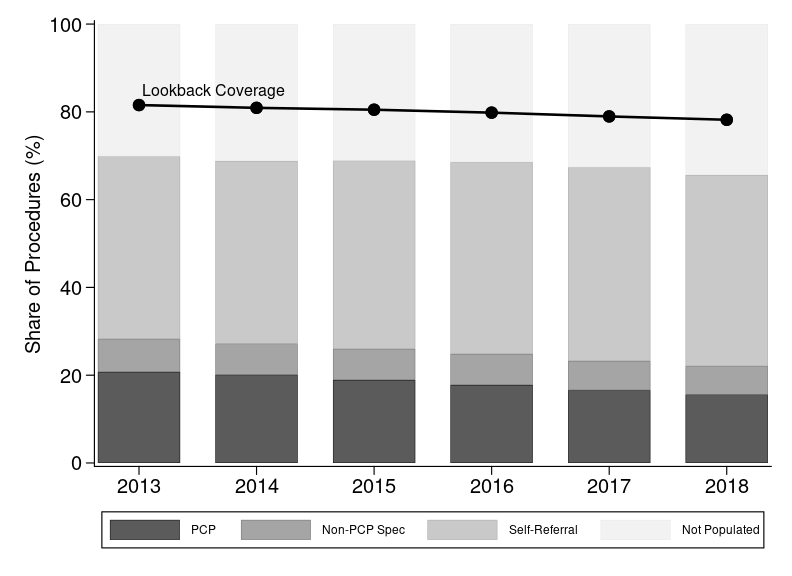
\includegraphics[width=5in]{../../../results/figures/desc/PCP_Validation_Figure.png}
}
\label{fig:pcp-validation}
\end{minipage}
\end{figure}

\clearpage
\begin{figure}[!ht]
\centering
\begin{minipage}[h]{6in}
\caption[Bias in $\hat\alpha$]{Bias in $\hat\alpha$ as a function of the true $\alpha$ and the base failure rate, with quality dispersion fixed at 0.03.\footnote{The surface is smoothed using a polynomial fit to the simulation grid. Darker shading indicates larger bias.}}
\centerline{%
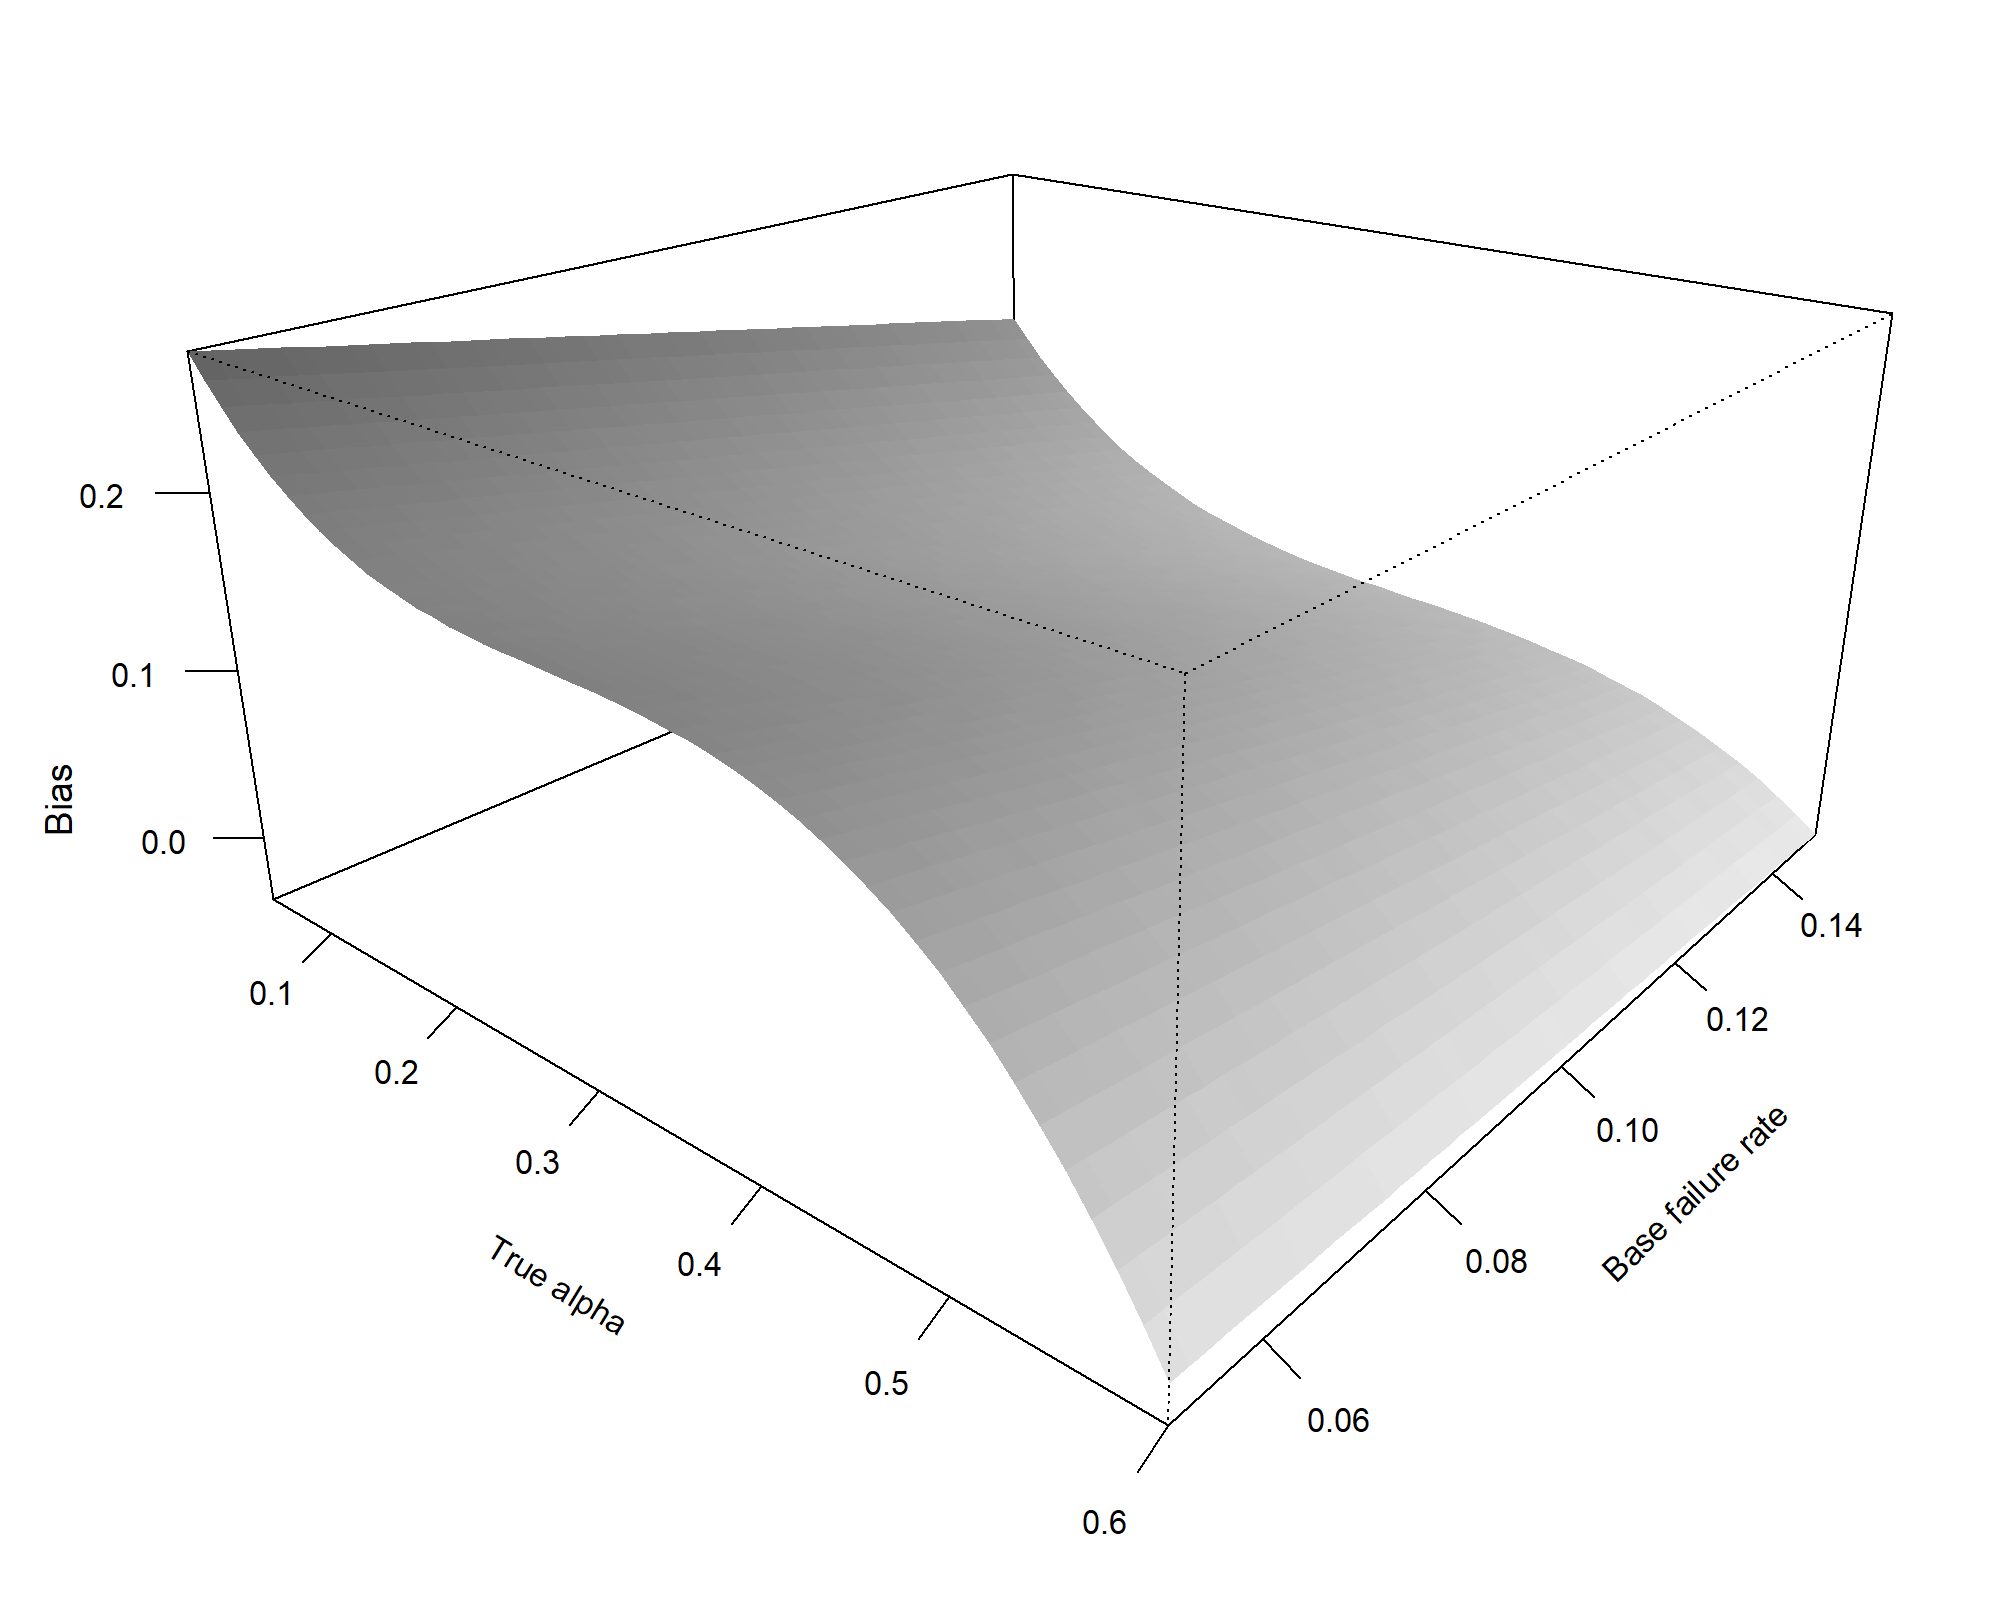
\includegraphics[width=5in]{../../../results/figures/simulation/fig-bias-surface.png}
}
\label{fig:bias-surface}
\end{minipage}
\end{figure}

\clearpage
\begin{figure}[!ht]
\centering
\begin{minipage}[h]{6in}
\caption[Relative bias in $\hat\alpha$]{Relative bias in $\hat\alpha$ (as a percentage of the true value) by base failure rate, with quality dispersion fixed at 0.03.\footnote{The shaded band marks $\pm$10\% relative bias. Arrows indicate values exceeding 150\% (truncated for readability).}}
\centerline{%
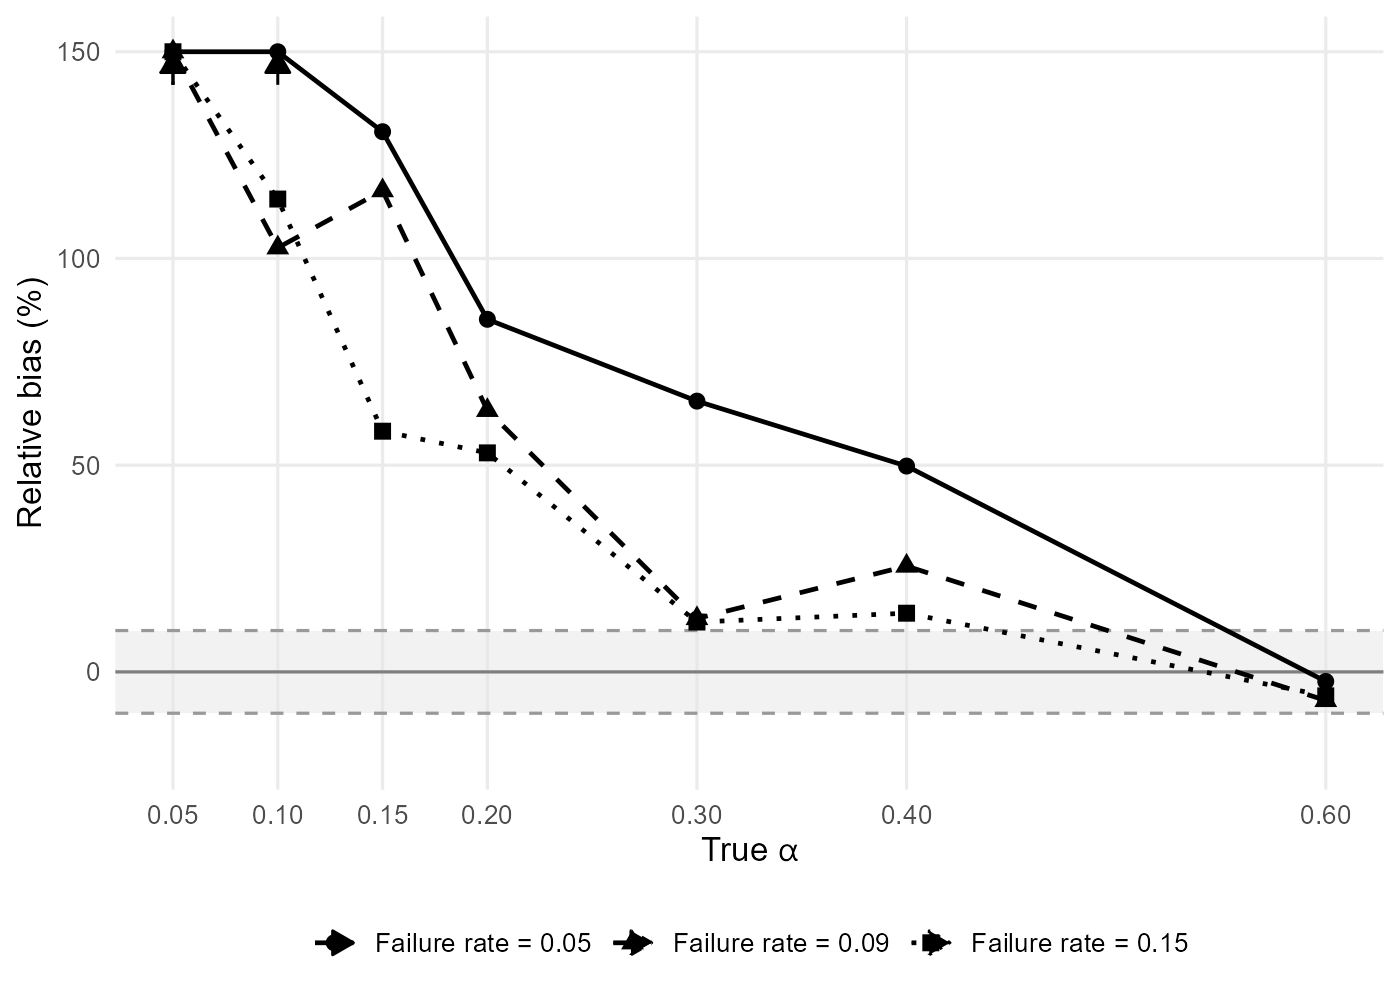
\includegraphics[width=5in]{../../../results/figures/simulation/fig-relbias-by-alpha.png}
}
\label{fig:relbias-alpha}
\end{minipage}
\end{figure}

\clearpage
\begin{figure}[!ht]
\centering
\begin{minipage}[h]{6in}
\caption[Log-Likelihood by $\eta$]{Log-Likelihood Values in Four Example Simulations\footnote{Plots of the log-likelihood (``lnL\_list'') against the candidate value of $\eta$ (``eta-hat,'' plotted on a log scale), from four example simulations. All other parameters are held at the values used to generate the simulated data, which consists of 2,500 patients and 25 specialists.}}
\begin{tabular}{cc}
\\
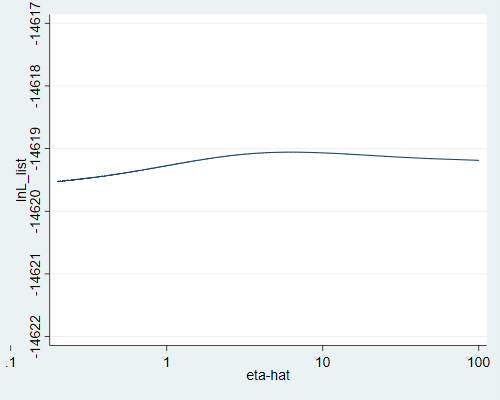
\includegraphics[scale=0.38]{../../../results/figures/simulation/like_eta_1.png} &
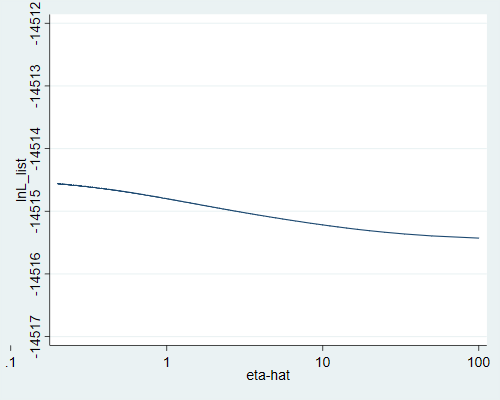
\includegraphics[scale=0.38]{../../../results/figures/simulation/like_eta_2.png} \\
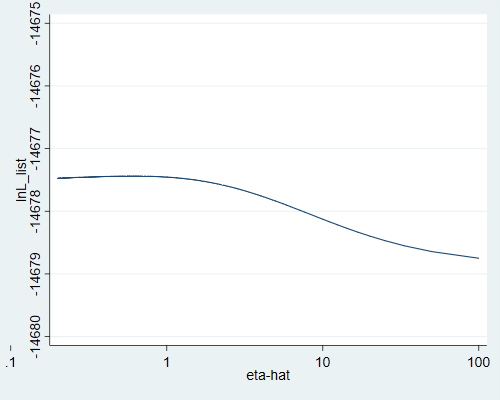
\includegraphics[scale=0.38]{../../../results/figures/simulation/like_eta_3.png} &
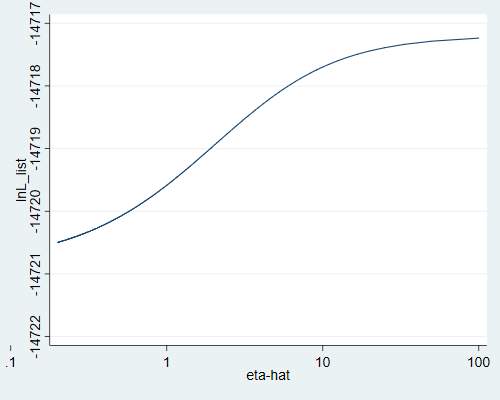
\includegraphics[scale=0.38]{../../../results/figures/simulation/like_eta_4.png}
\end{tabular}
\label{fig:eta-simulation}
\end{minipage}
\end{figure}

\clearpage
\begin{figure}[!ht]
\centering
\begin{minipage}[h]{6in}
\caption[First-Stage Partial Scatter]{Partial scatter plots of actual versus predicted patient counts, residualized on HRR fixed effects and a time-period indicator.\footnote{Each point represents a specialist-time period observation, weighted by the inverse variance of the specialist fixed effect. The fitted line shows the first-stage relationship. Left panel shows $\eta=1$, right panel shows $\eta=5$.}}
\begin{tabular}{cc}
\\
$\eta=1$ & $\eta=5$ \\
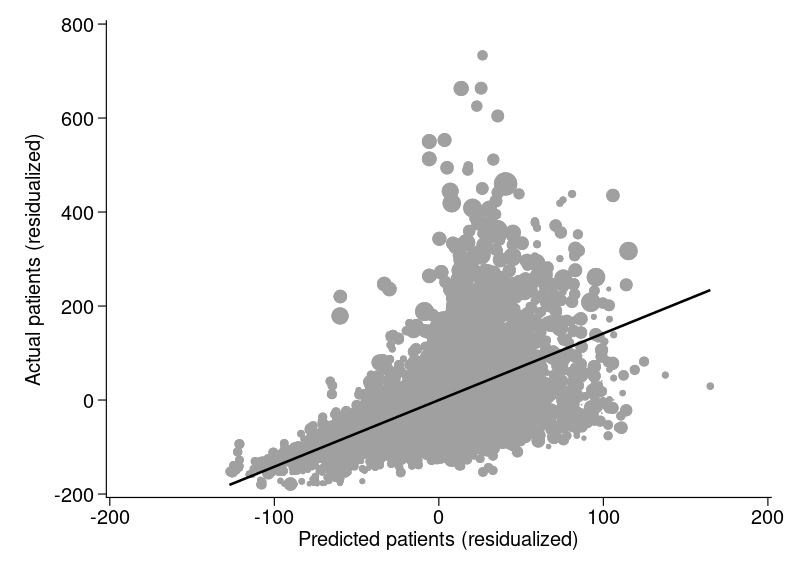
\includegraphics[height=3in,width=2.7in,keepaspectratio]{../../../results/figures/myopic-timevary/FirstStage_Scatter_Myopic_eta1_1_1_0.png} & 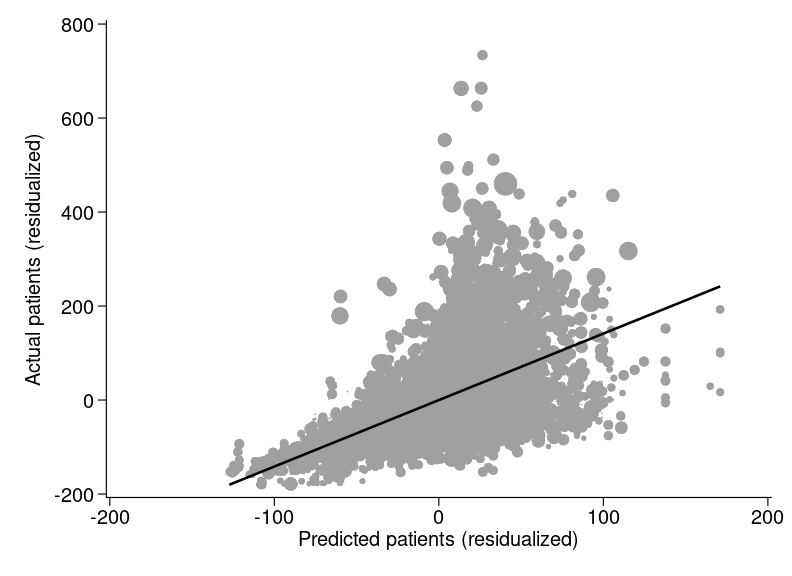
\includegraphics[height=3in,width=2.7in,keepaspectratio]{../../../results/figures/myopic-timevary/FirstStage_Scatter_Myopic_eta5_1_1_0.png}
\end{tabular}
\label{fig:fs-scatter}
\end{minipage}
\end{figure}

\clearpage
\begin{figure}[!ht]
\centering
\begin{minipage}[h]{6in}
\caption[First-Stage F-Statistics]{Distribution of HRR-level first-stage F-statistics, weighted by patient volume.\footnote{Dashed line marks the conventional threshold of $F=10$. Each HRR-level regression includes the distance-based instrument, a time-period indicator, and is weighted by the inverse variance of the specialist fixed effect. Left panel shows $\eta=1$, right panel shows $\eta=5$.}}
\begin{tabular}{cc}
\\
$\eta=1$ & $\eta=5$ \\
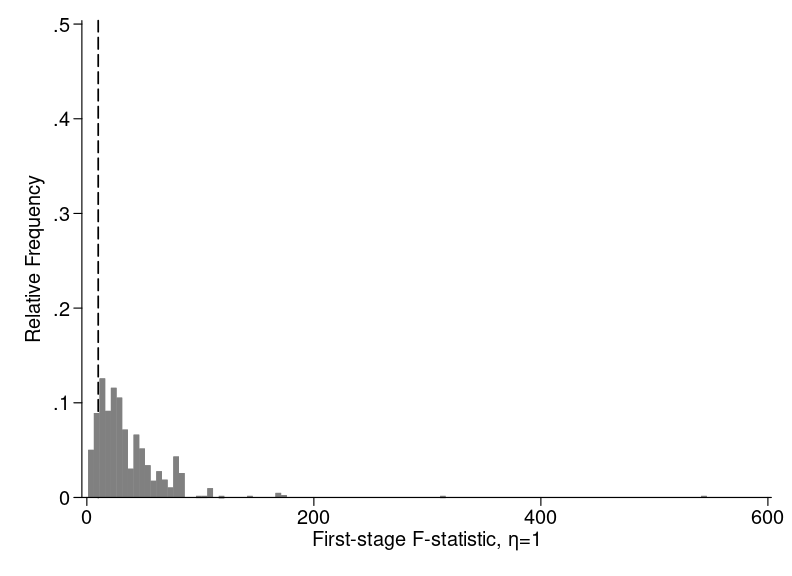
\includegraphics[height=3in,width=2.7in,keepaspectratio]{../../../results/figures/myopic-timevary/FirstStage_Fstat_Myopic_eta1_1_1_0.png} & 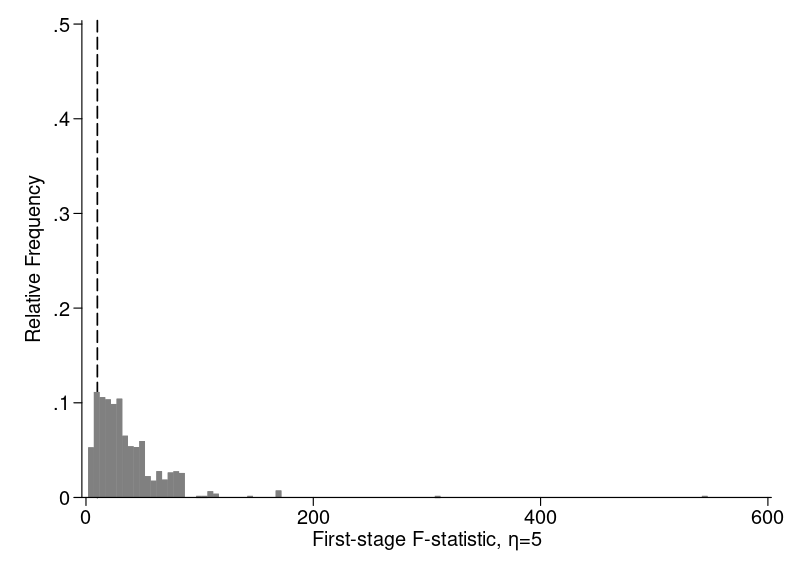
\includegraphics[height=3in,width=2.7in,keepaspectratio]{../../../results/figures/myopic-timevary/FirstStage_Fstat_Myopic_eta5_1_1_0.png}
\end{tabular}
\label{fig:fs-fstat}
\end{minipage}
\end{figure}

\clearpage
\begin{figure}[!ht]
\centering
\begin{minipage}[h]{6in}
\caption[Predicted vs Actual Shares]{Predicted versus Actual Referral Shares ($\eta=1$)\footnote{Each point is a specialist-period observation. The horizontal axis is the actual share of referrals the specialist receives in an HRR-period; the vertical axis is the model-predicted share. The 45-degree line is shown in black.}}
\begin{tabular}{cc}
\\
Myopic & Forward-looking \\
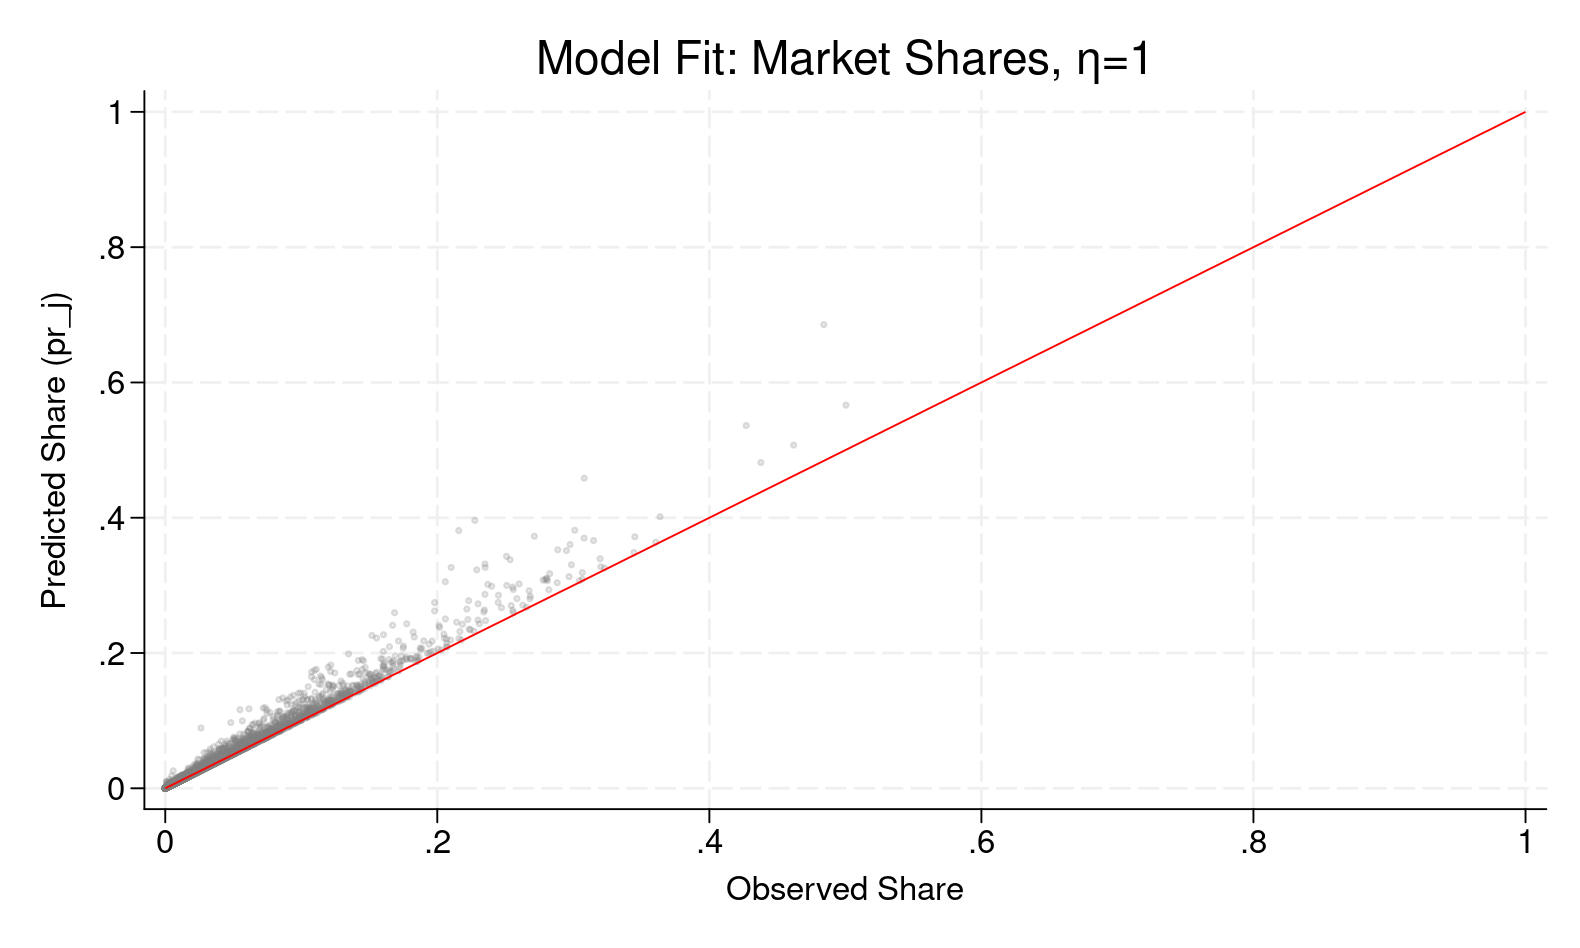
\includegraphics[height=3in,width=2.7in,keepaspectratio]{../../../results/figures/myopic-timevary/_est-diag-fit-shares_Myopic_eta1.png} & 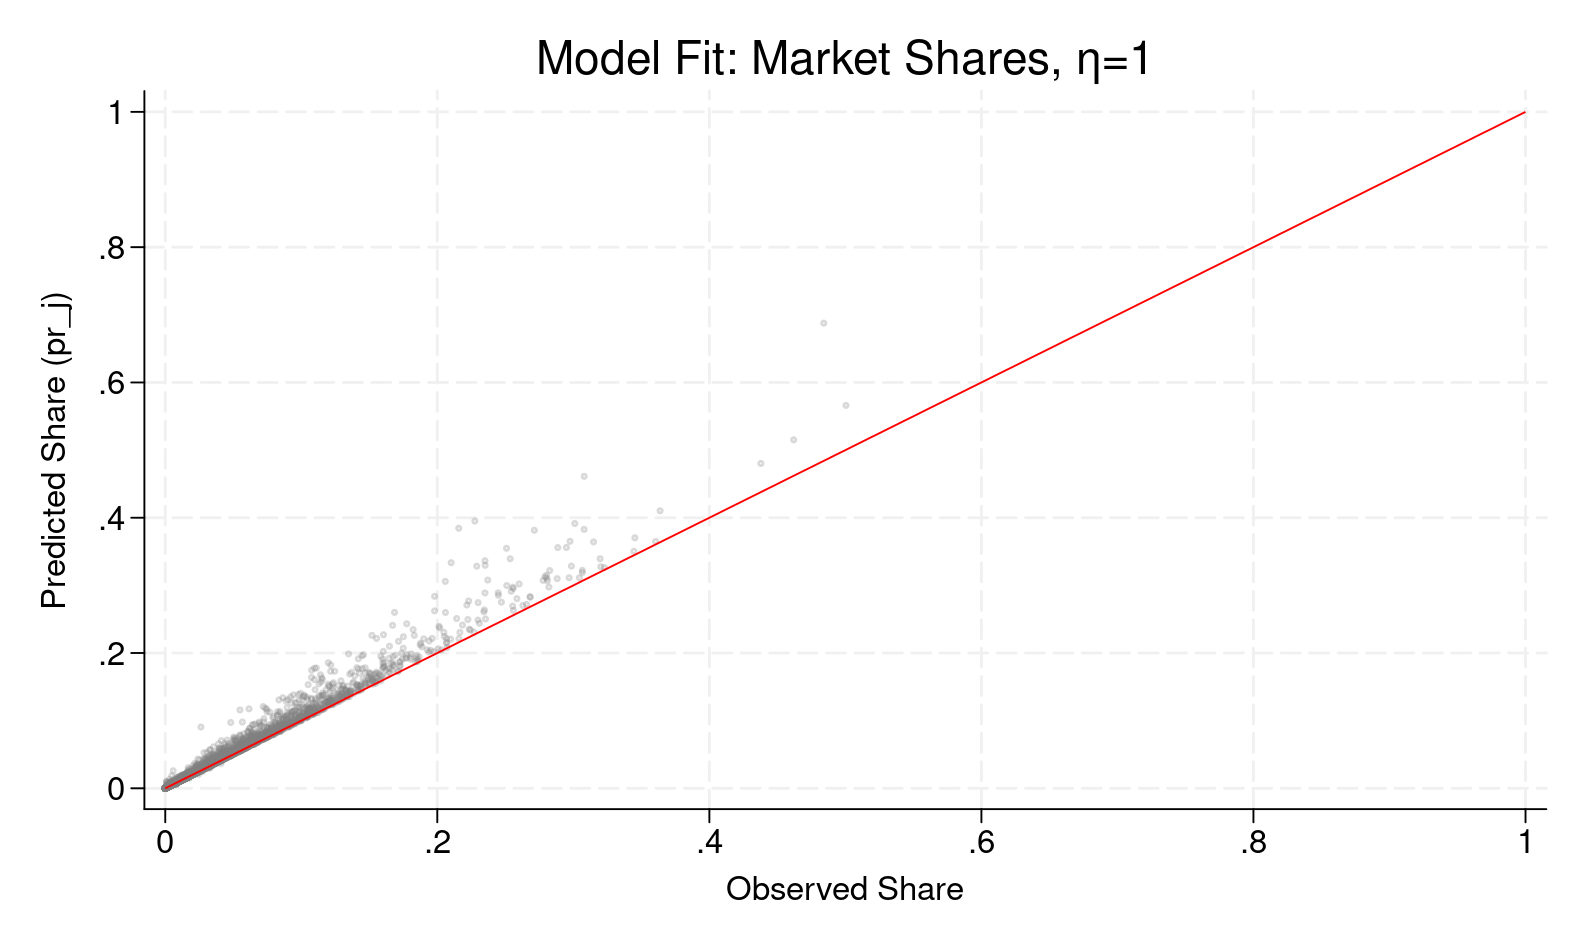
\includegraphics[height=3in,width=2.7in,keepaspectratio]{../../../results/figures/fwd-timevary/_est-diag-fit-shares_FWD_eta1.png}
\end{tabular}
\label{fig:fit-shares}
\end{minipage}
\end{figure}

\clearpage
\begin{figure}[!ht]
\centering
\begin{minipage}[h]{6in}
\caption[FE vs Quality]{Specialist Fixed Effects and Observed Quality ($\eta=1$)\footnote{Each point is a specialist. The horizontal axis is observed specialist quality (success rate); the vertical axis is the estimated specialist fixed effect $\xi_j$ from the structural model. Within-HRR variation is the basis for the structural interpretation of $\alpha$, so near-zero within-HRR correlation between $\xi_j$ and quality supports the separate identification of the learning channel.}}
\begin{tabular}{cc}
\\
Myopic & Forward-looking \\
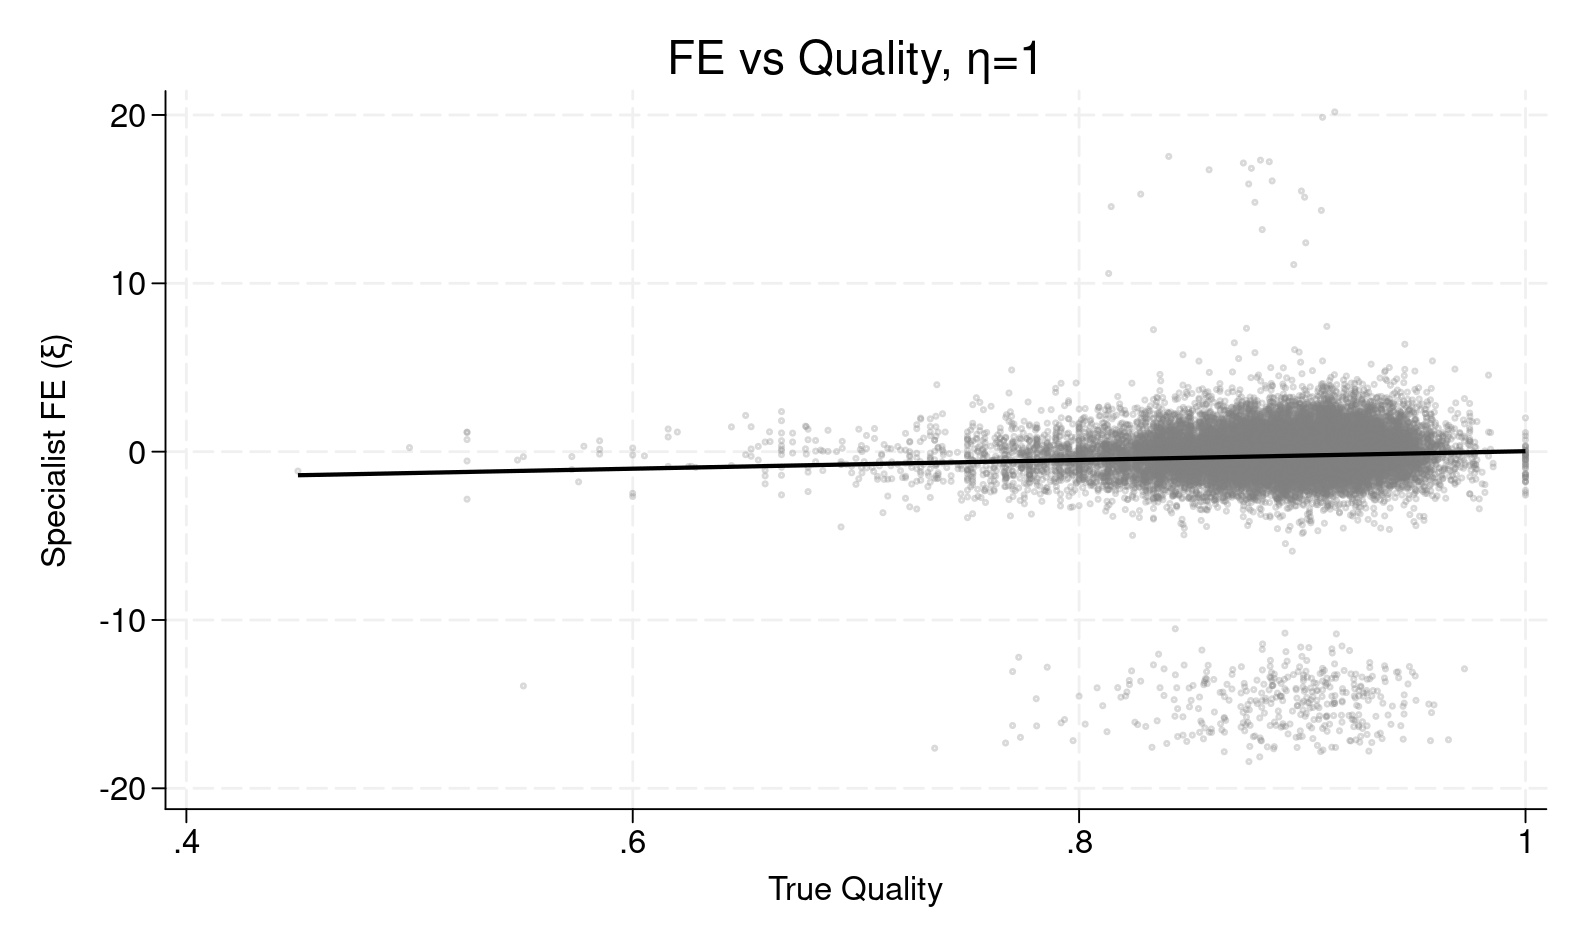
\includegraphics[height=3in,width=2.7in,keepaspectratio]{../../../results/figures/myopic-timevary/_est-diag-fe-quality_Myopic_eta1.png} & 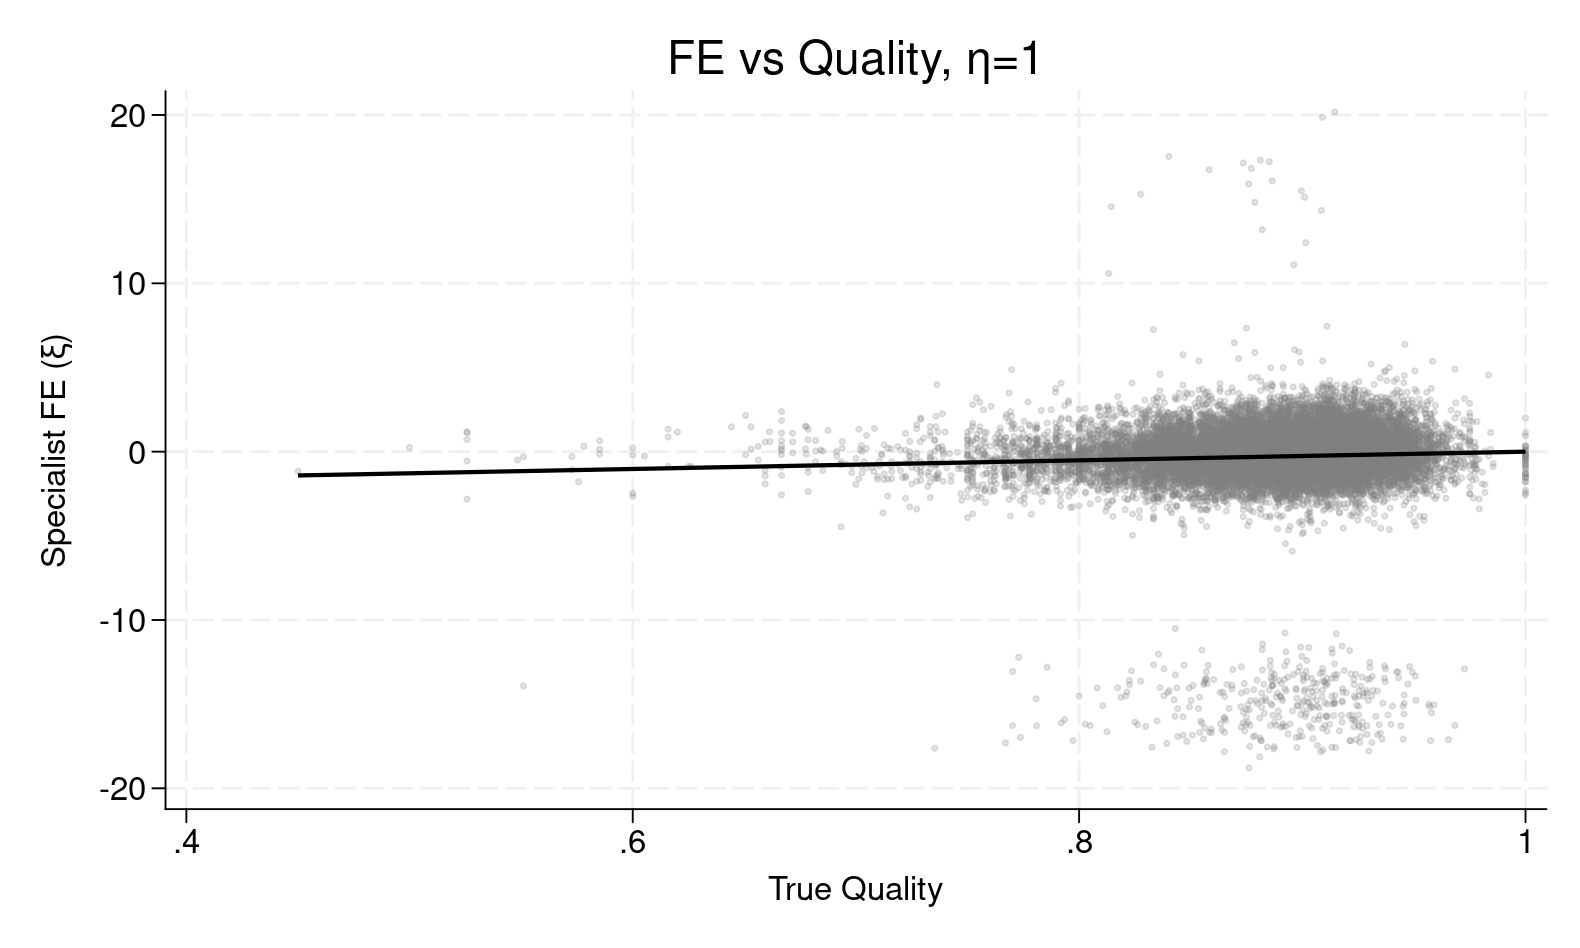
\includegraphics[height=3in,width=2.7in,keepaspectratio]{../../../results/figures/fwd-timevary/_est-diag-fe-quality_FWD_eta1.png}
\end{tabular}
\label{fig:fe-quality}
\end{minipage}
\end{figure}

\clearpage
\begin{figure}[!ht]
\centering
\begin{minipage}[h]{6in}
\caption[Event Studies by Cohort]{Event Studies by Failure Cohort\footnote{Figure depicts event study estimates following \cite{cengiz2019}, based on Equation 1 of the main text, estimated separately by failure cohort (e.g., first failure, second failure, etc.). Our specification includes specialist X quarter fixed effects as well as an indicator for PCP `type'. The event study coefficient at time $\tau = -1$ is normalized to 0.}}
\begin{tabular}{cc}
\\
First Failure & Second Failure \\
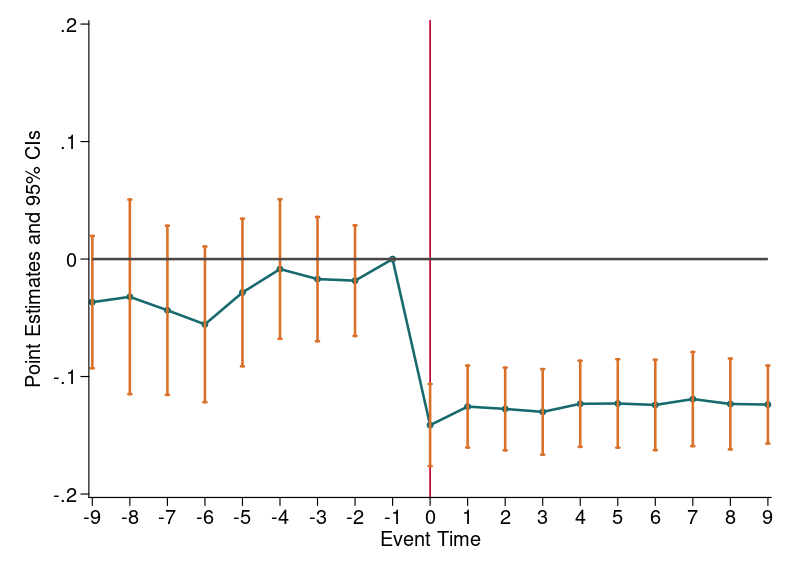
\includegraphics[height=3in,width=2.7in,keepaspectratio]{../../../results/figures/rf/EventStudy_Group1_1_1_0.png} & 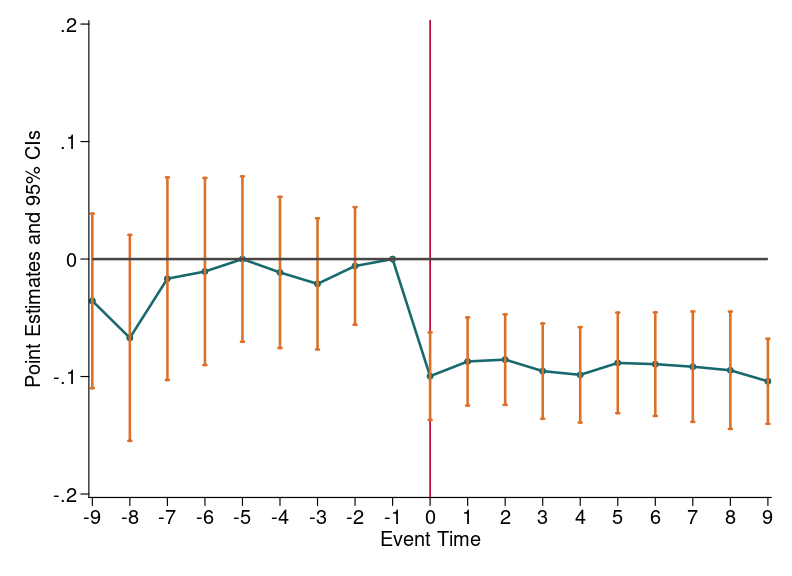
\includegraphics[height=3in,width=2.7in,keepaspectratio]{../../../results/figures/rf/EventStudy_Group2_1_1_0.png} \\
Third Failure & Fourth Failure \\
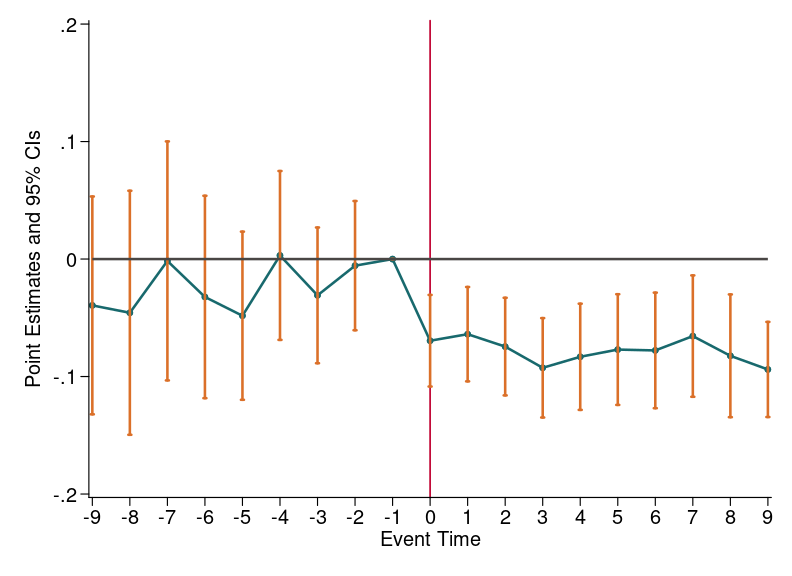
\includegraphics[height=3in,width=2.7in,keepaspectratio]{../../../results/figures/rf/EventStudy_Group3_1_1_0.png} & 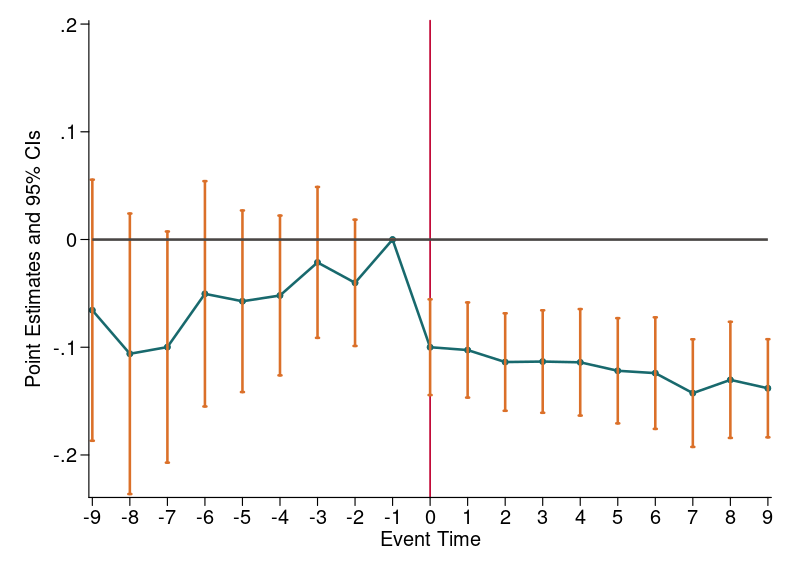
\includegraphics[height=3in,width=2.7in,keepaspectratio]{../../../results/figures/rf/EventStudy_Group4_1_1_0.png}
\end{tabular}
\label{fig:event-cohort}
\end{minipage}
\end{figure}

\clearpage
\begin{figure}[!ht]
\centering
\begin{minipage}[h]{6in}
\caption[Full Information, No Familiarity]{Counterfactuals from Full Information and No Familiarity\footnote{Figure depicts the share of referrals reallocated and the resulting effects on patient health (i.e., the change in the probability of a successful surgery) under a counterfactual in which PCPs have full information about specialist quality and do not incorporate any familiarity in their referral decisions. Estimates are averaged across individuals within an HRR and presented as a histogram across HRRs. Results limited to HRRs in which our constrained maximization routine converged, \nHRRsMyopic{} (\nHRRsFWD{}) HRRs in the myopic (forward-looking) case for $\eta=1$ and \nHRRsEtaFiveMyopic{} (\nHRRsEtaFiveFWD{}) in the myopic (forward-looking) case for $\eta=5$.}}
\centerline{%
\begin{tabular}{cc}
\\
\multicolumn{2}{c}{\textit{Myopic Referrals, Reallocation}} \\
$\eta=1$ & $\eta=5$ \\
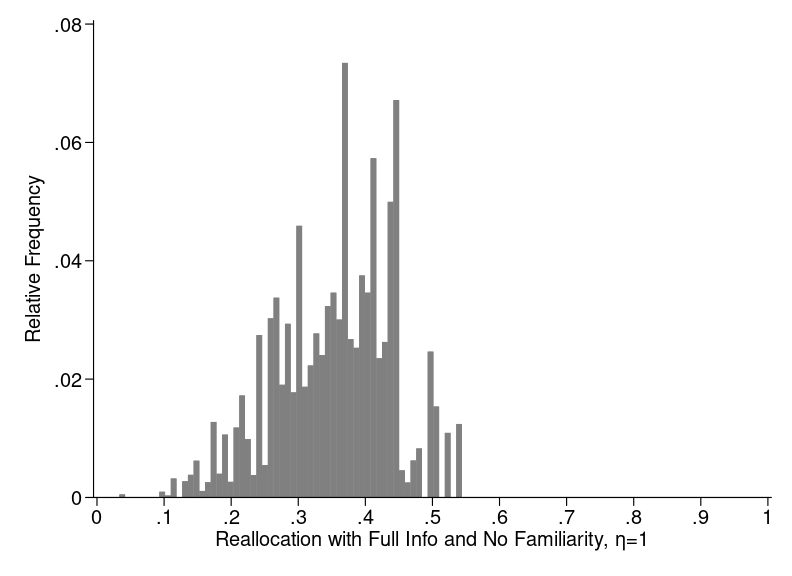
\includegraphics[height=1.35in,width=2.5in,keepaspectratio]{../../../results/figures/myopic-timevary/Reallocation_FullFam_Myopic_eta1.png} & 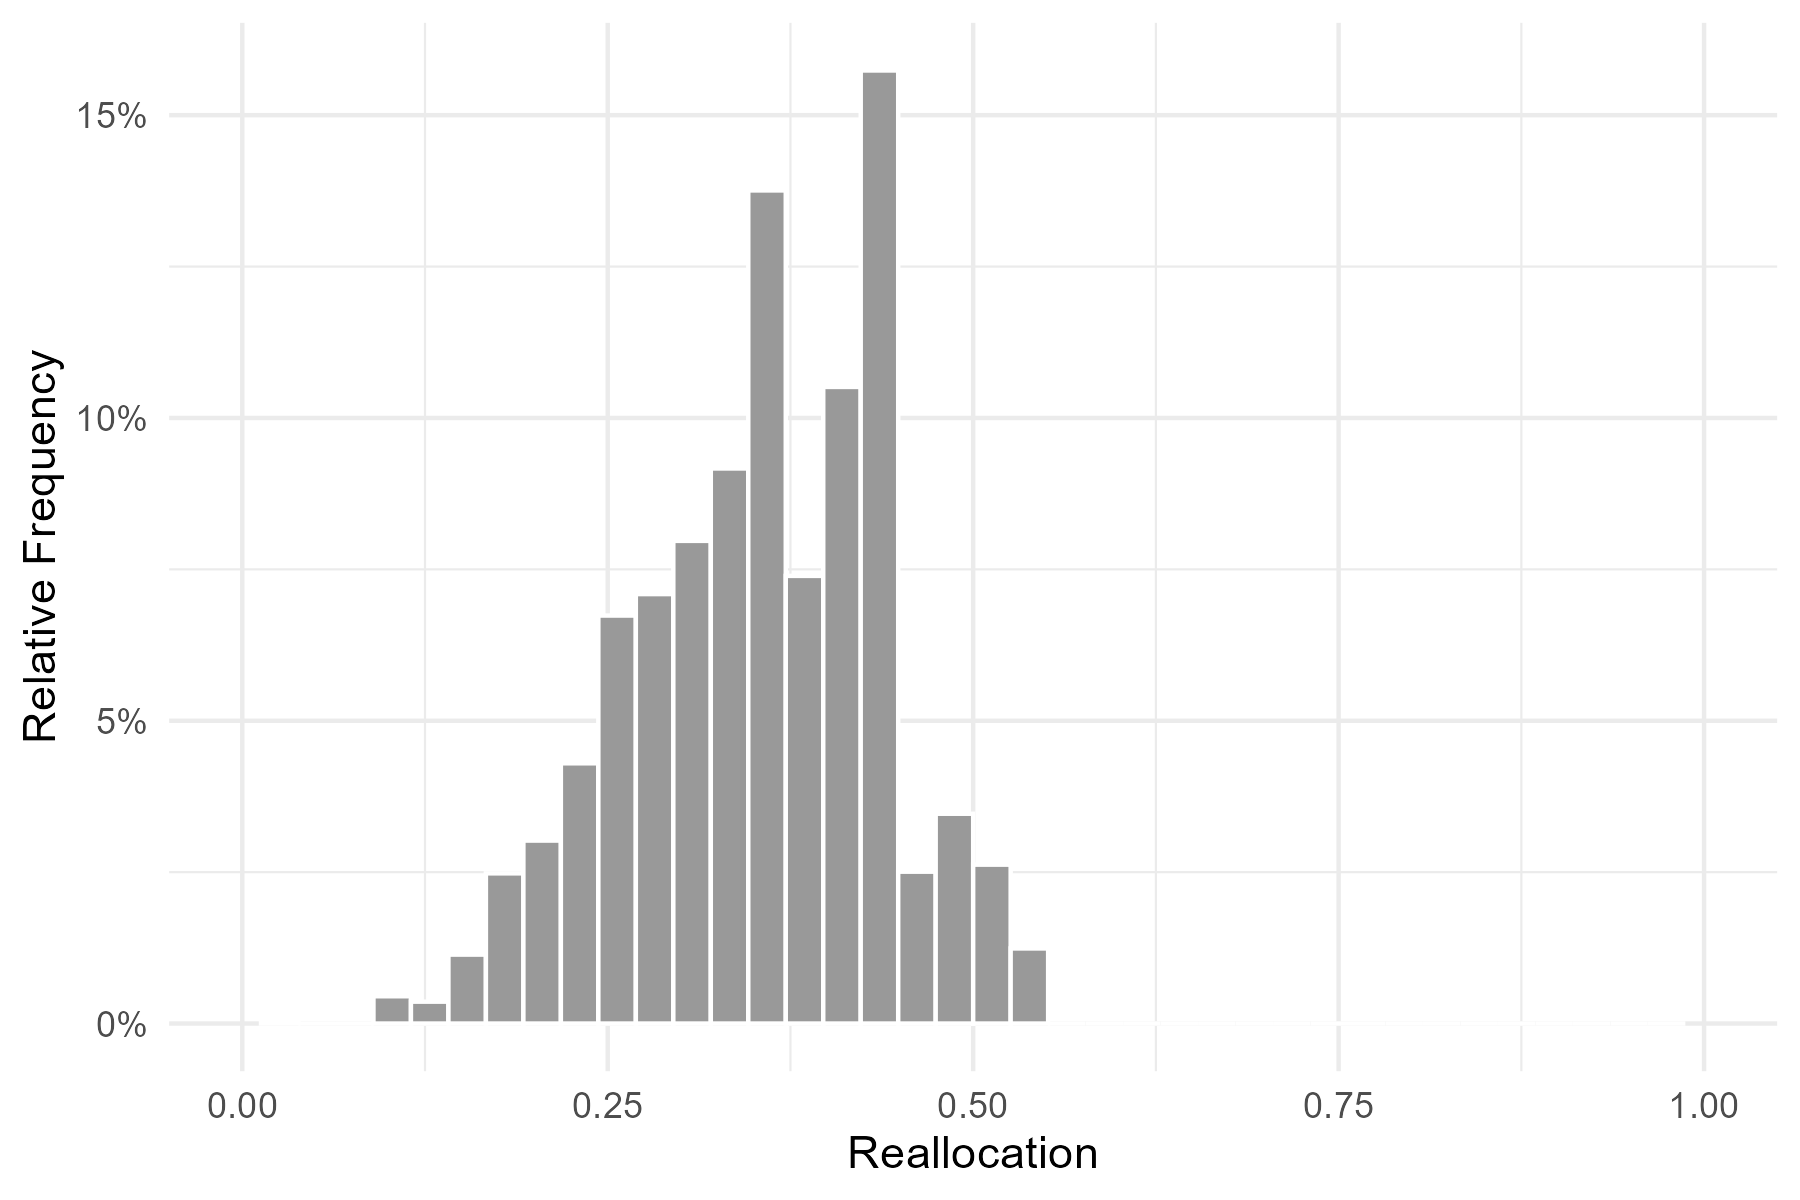
\includegraphics[height=1.35in,width=2.5in,keepaspectratio]{../../../results/figures/myopic-timevary/Reallocation_FullFam_Myopic_eta5.png} \\
\multicolumn{2}{c}{\textit{Myopic Referrals, Health Improvements}} \\
$\eta=1$ & $\eta=5$ \\
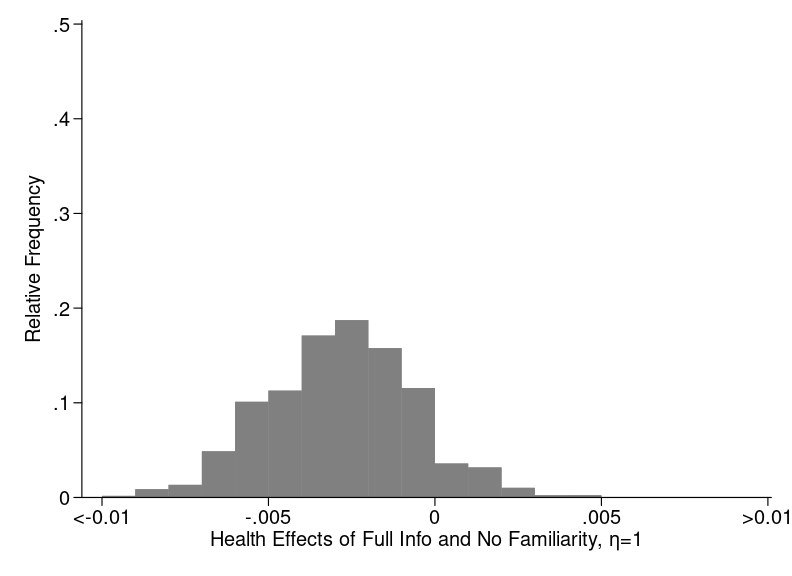
\includegraphics[height=1.35in,width=2.5in,keepaspectratio]{../../../results/figures/myopic-timevary/Mean_Health_FX_FullFam_Myopic_eta1.png} & 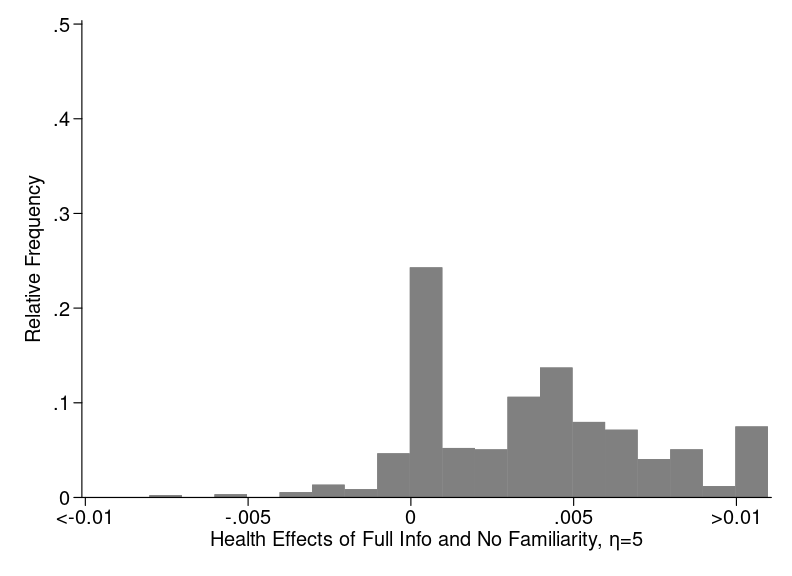
\includegraphics[height=1.35in,width=2.5in,keepaspectratio]{../../../results/figures/myopic-timevary/Mean_Health_FX_FullFam_Myopic_eta5.png} \\
\multicolumn{2}{c}{\textit{Forward-looking Referrals, Reallocation}} \\
$\eta=1$ & $\eta=5$ \\
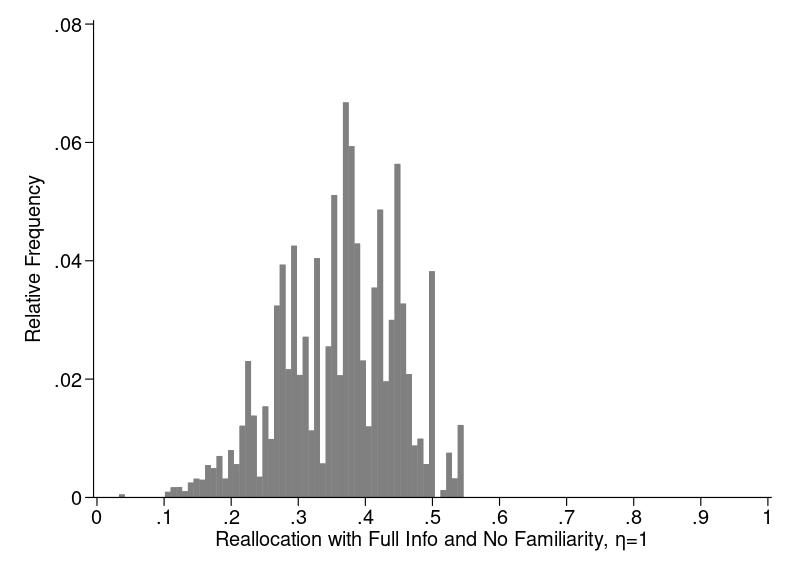
\includegraphics[height=1.35in,width=2.5in,keepaspectratio]{../../../results/figures/fwd-timevary/Reallocation_FullFam_FWD_eta1.png} & 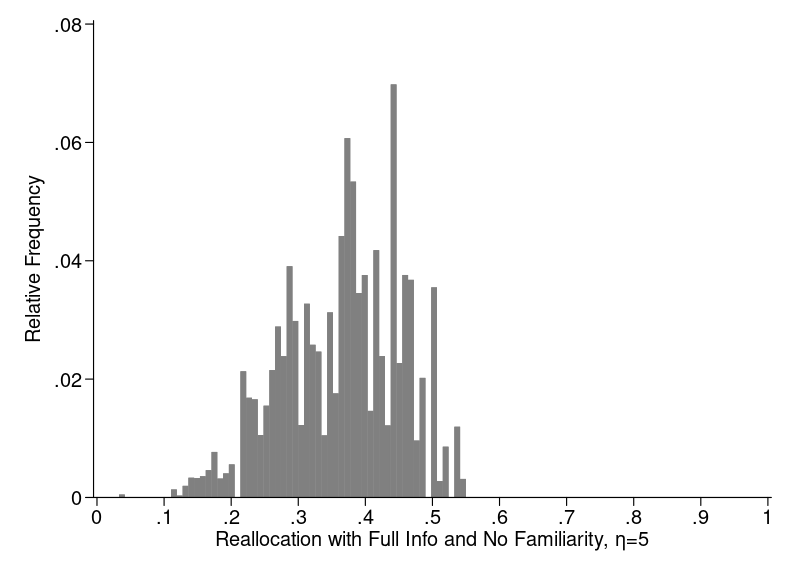
\includegraphics[height=1.35in,width=2.5in,keepaspectratio]{../../../results/figures/fwd-timevary/Reallocation_FullFam_FWD_eta5.png} \\
\multicolumn{2}{c}{\textit{Forward-looking Referrals, Health Improvements}} \\
$\eta=1$ & $\eta=5$ \\
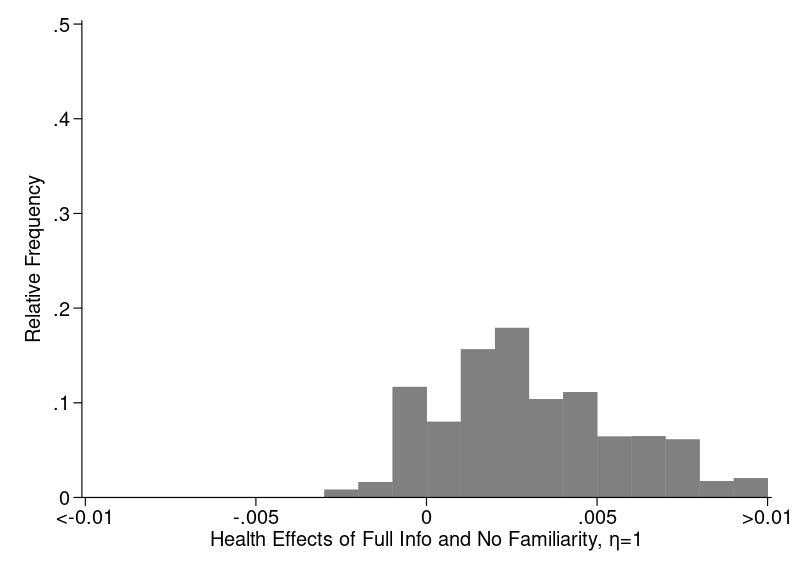
\includegraphics[height=1.35in,width=2.5in,keepaspectratio]{../../../results/figures/fwd-timevary/Mean_Health_FX_FullFam_FWD_eta1.png} & 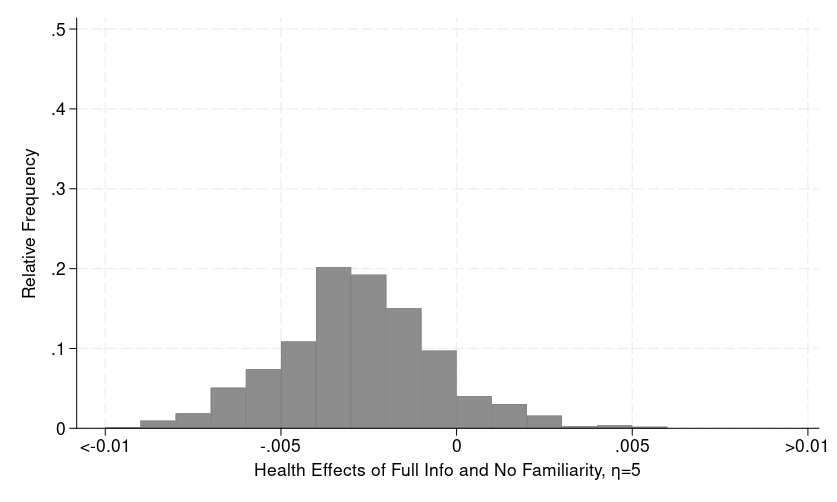
\includegraphics[height=1.35in,width=2.5in,keepaspectratio]{../../../results/figures/fwd-timevary/Mean_Health_FX_FullFam_FWD_eta5.png}
\end{tabular}}
\label{fig:cf_fullfam}
\end{minipage}
\end{figure}

\clearpage
\begin{figure}[!ht]
\centering
\begin{minipage}[h]{6in}
\caption[QualP10 Off-Diagonal]{Off-Diagonal Scatter of Patient-Weighted 10th-Percentile Quality ($\eta=1$)\footnote{Each point is an HRR where the patient-weighted 10th percentile of specialist quality under the counterfactual differs from the baseline value. HRRs with identical baseline and counterfactual percentile are dropped (they lie on the 45-degree line). The solid reference line is the 45-degree line.}}
\centering
\begin{tabular}{cc}
\multicolumn{2}{c}{\textit{Myopic}} \\
Existing familiarity & Reset familiarity \\
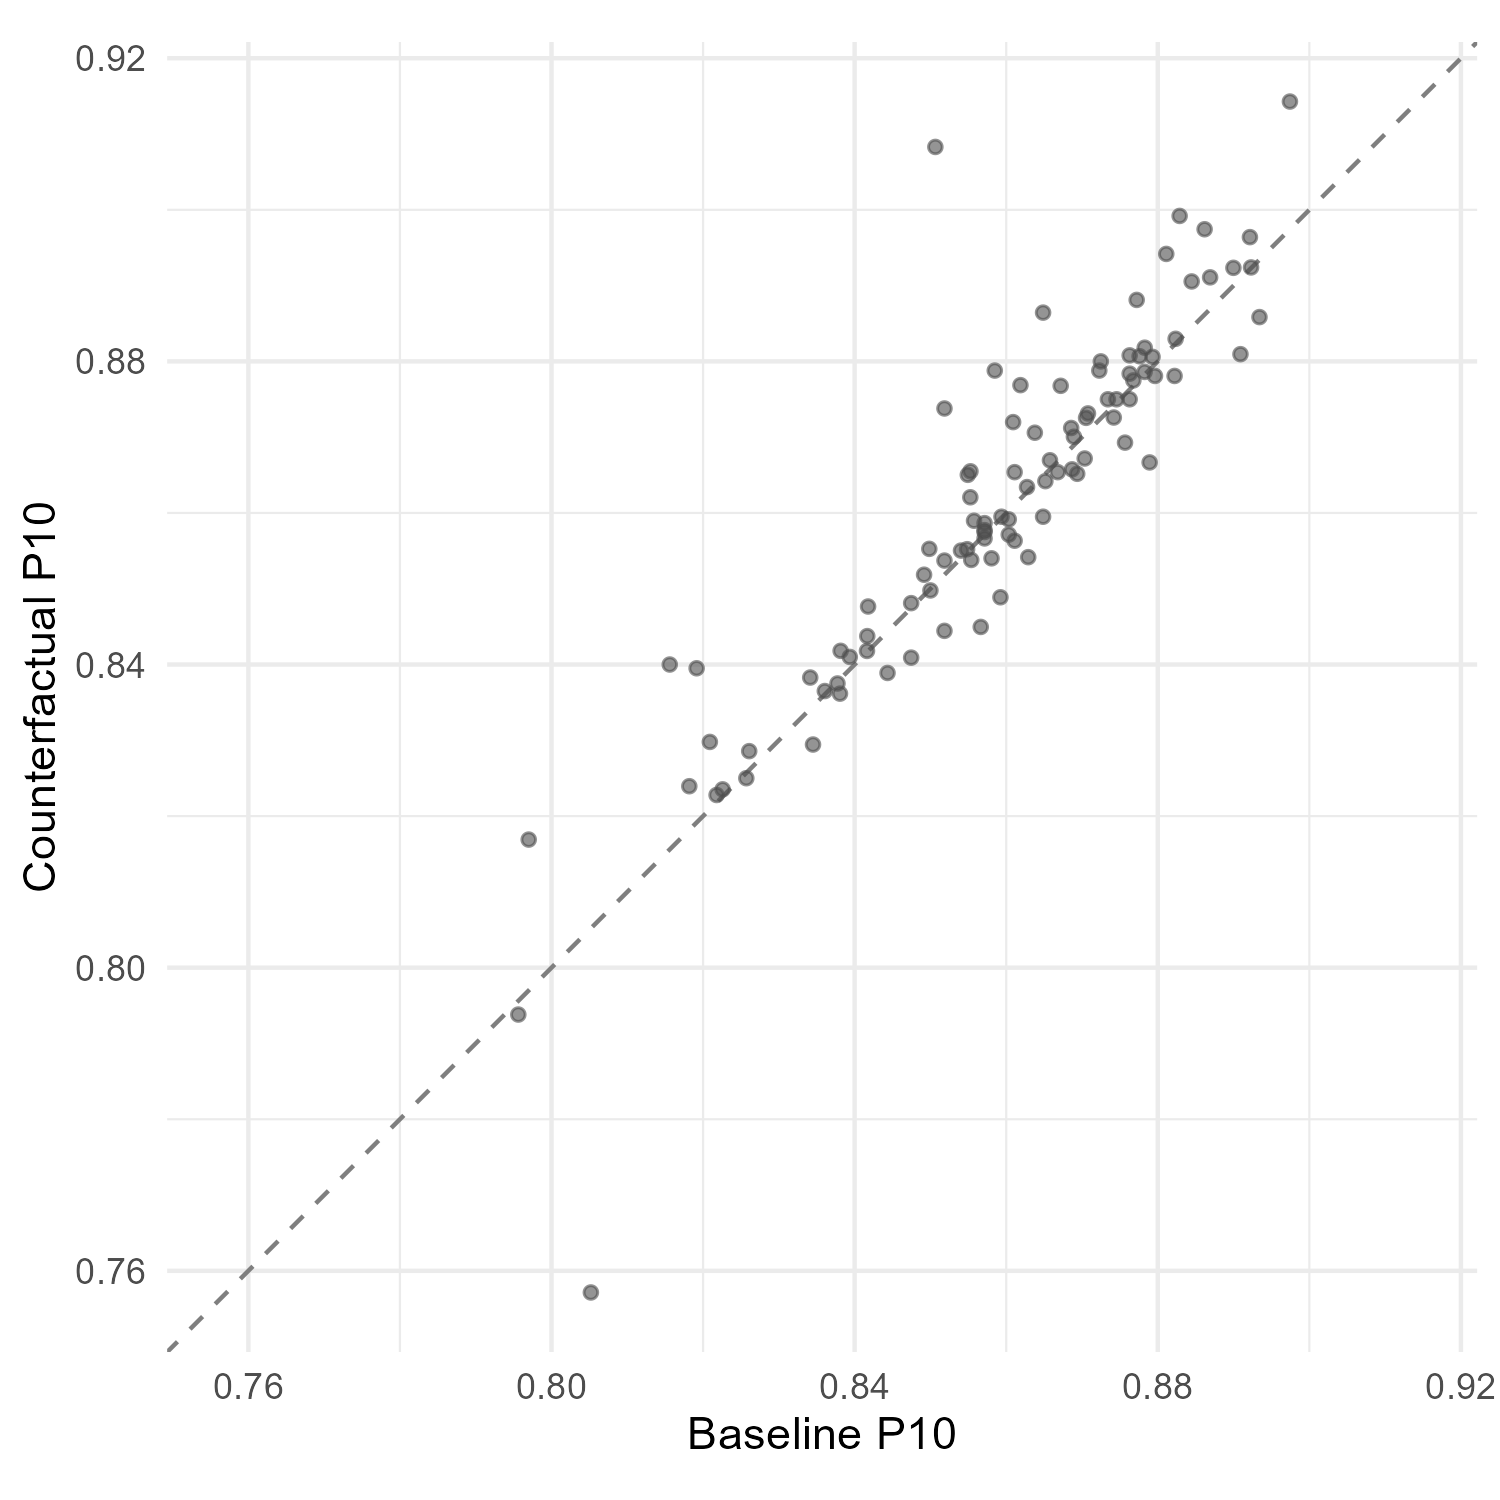
\includegraphics[height=2.2in,width=2.5in,keepaspectratio]{../../../results/figures/myopic-timevary/QualOffDiag_P10_current_Myopic_eta1.png} & 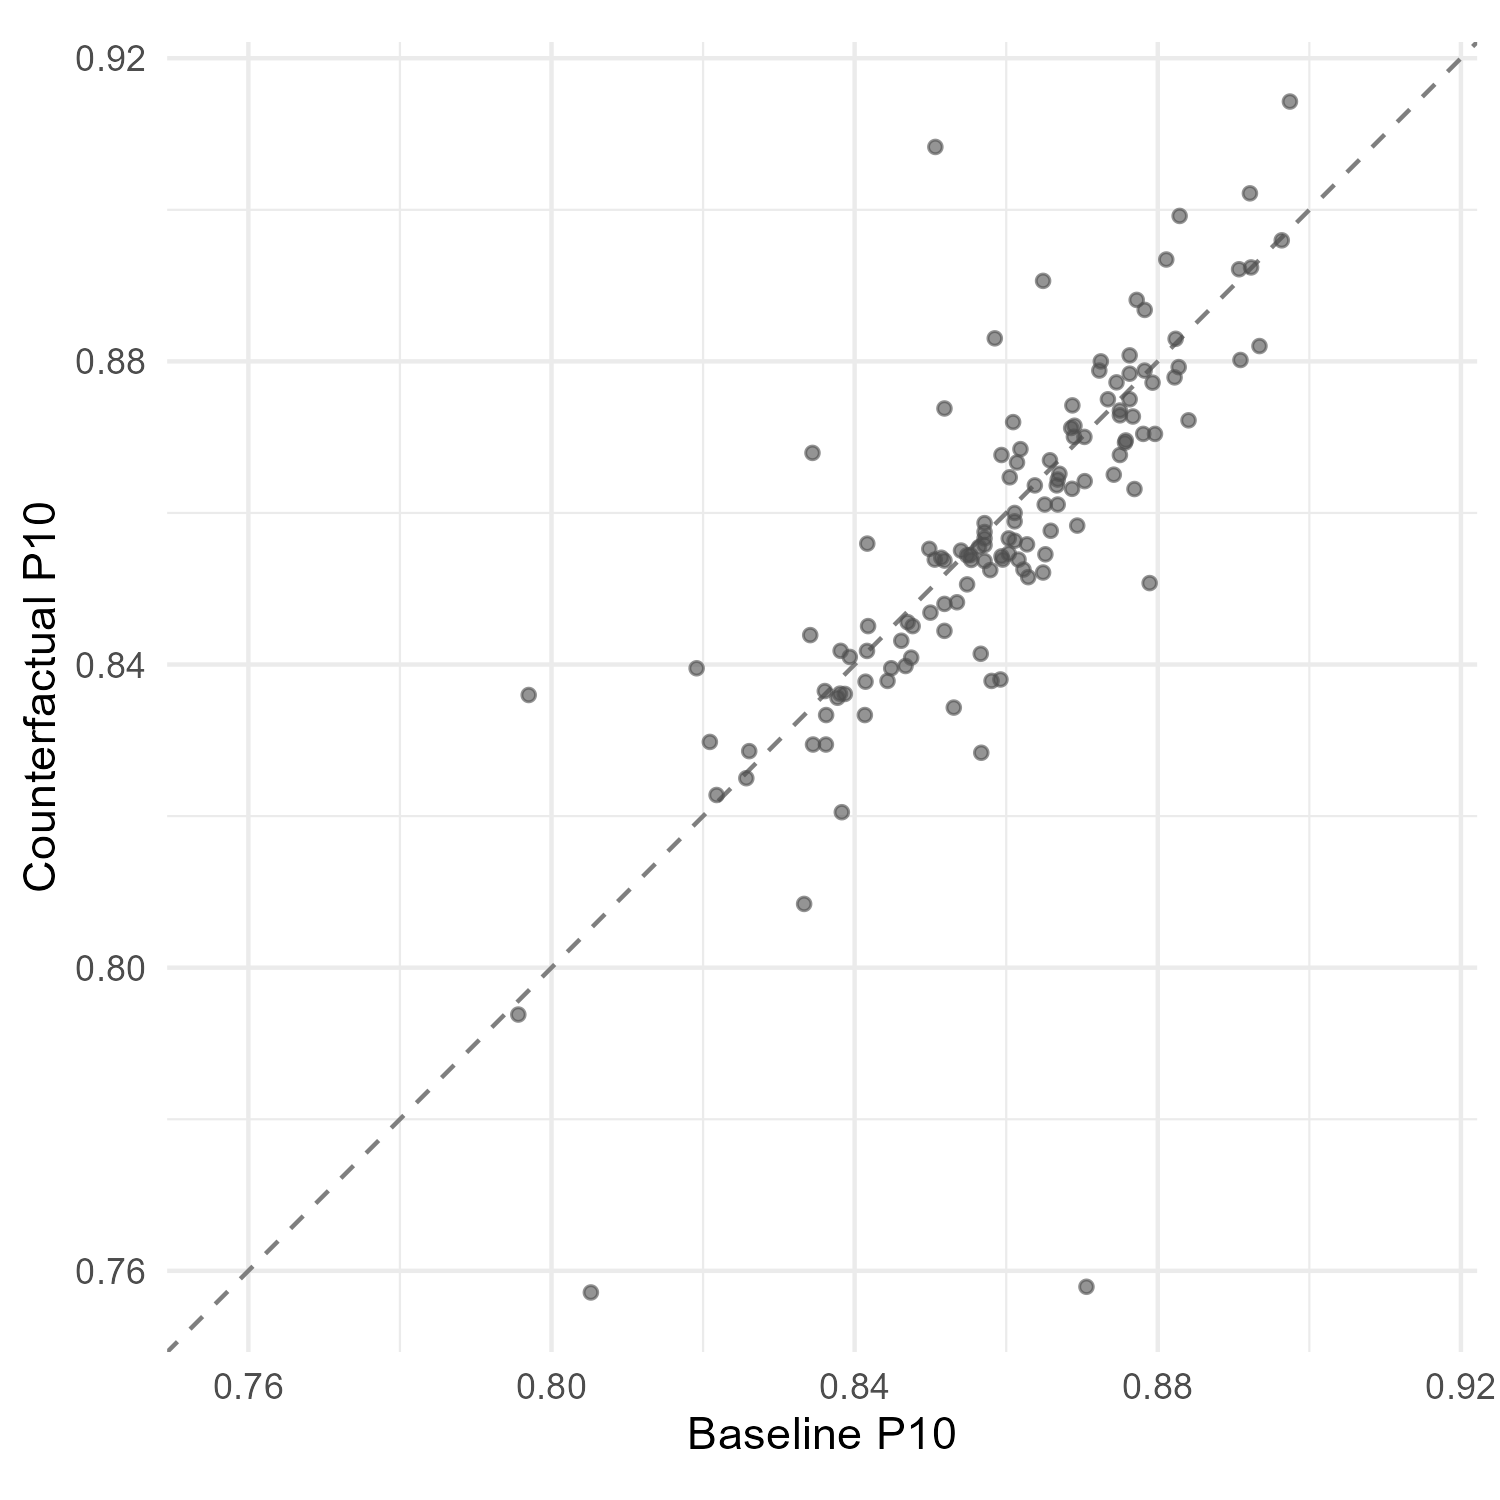
\includegraphics[height=2.2in,width=2.5in,keepaspectratio]{../../../results/figures/myopic-timevary/QualOffDiag_P10_full_Myopic_eta1.png} \\
\multicolumn{2}{c}{\textit{Forward-looking}} \\
Existing familiarity & Reset familiarity \\
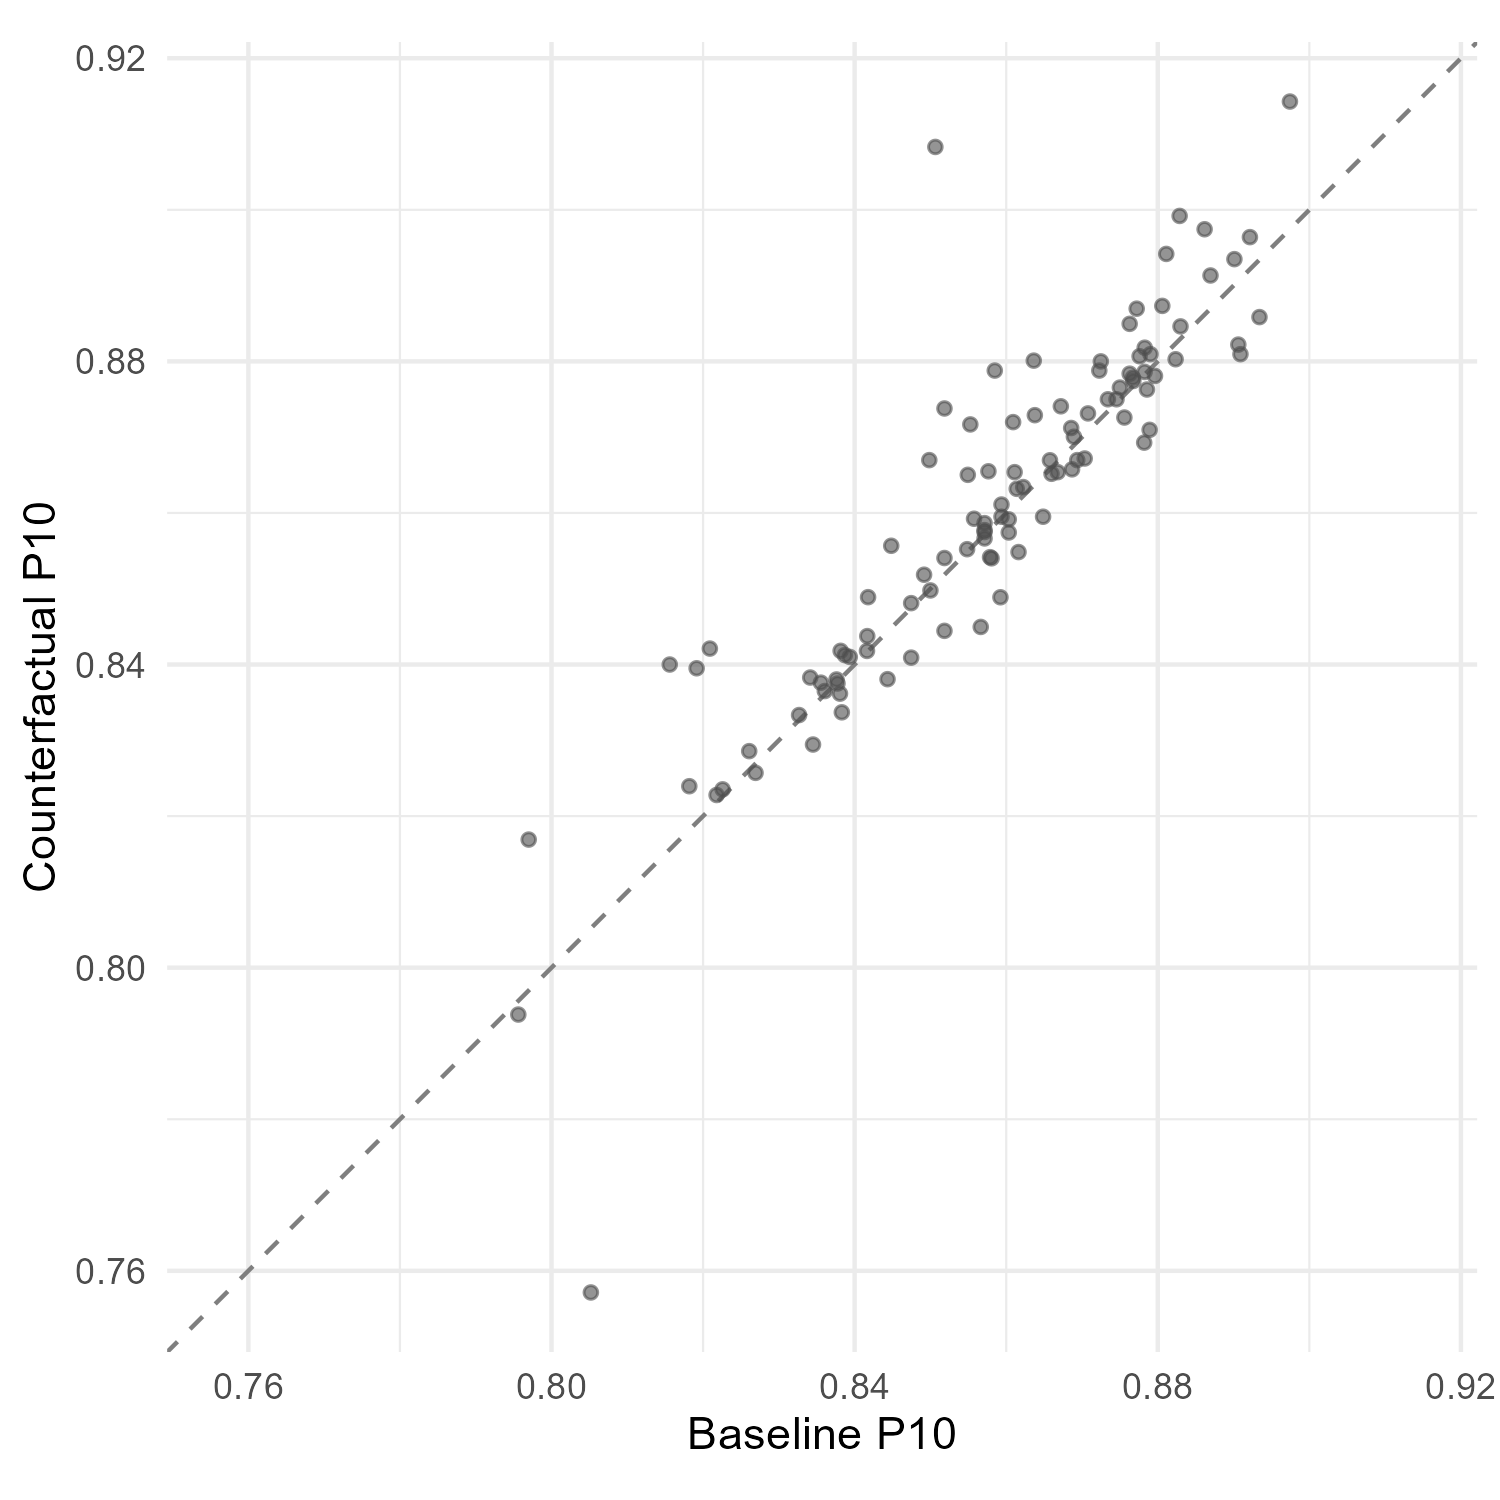
\includegraphics[height=2.2in,width=2.5in,keepaspectratio]{../../../results/figures/fwd-timevary/QualOffDiag_P10_current_FWD_eta1.png} & 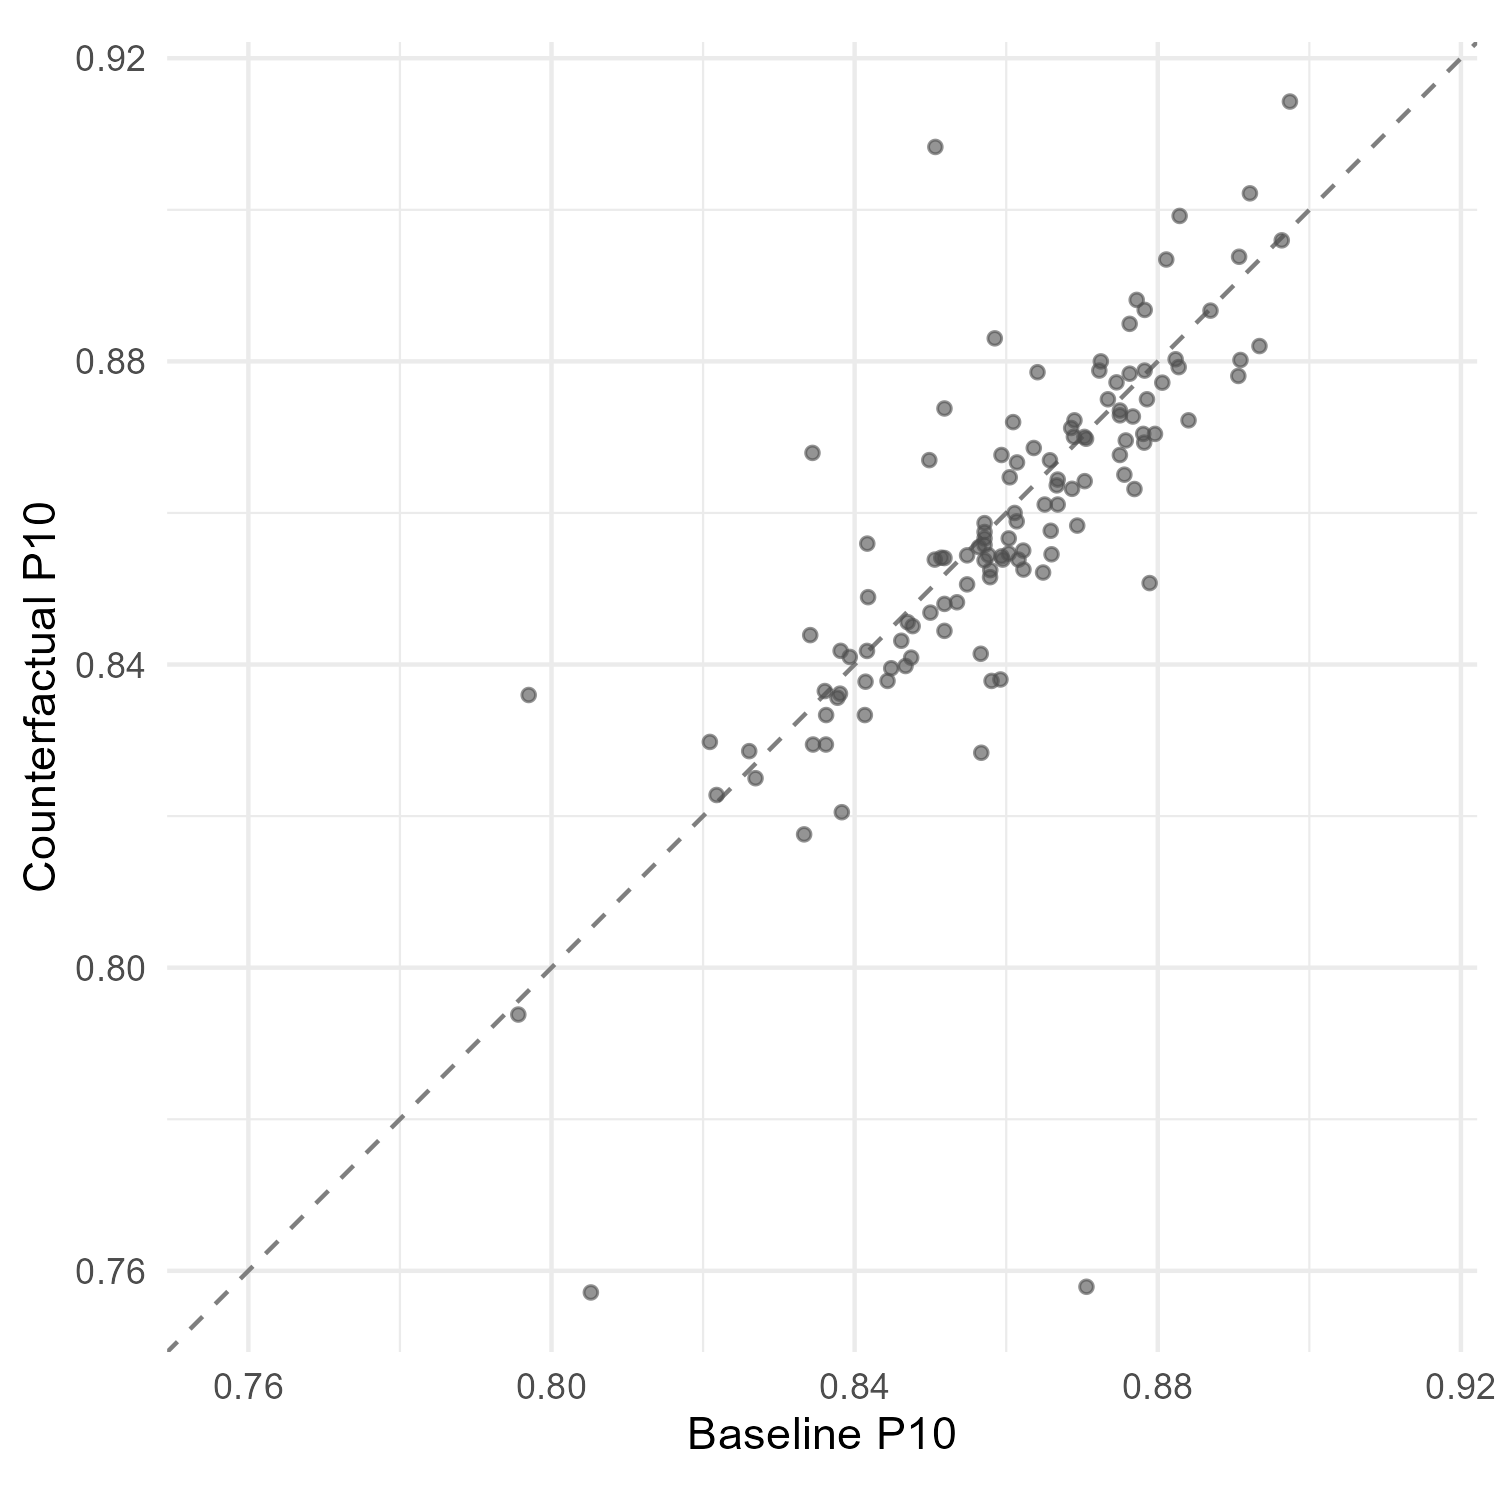
\includegraphics[height=2.2in,width=2.5in,keepaspectratio]{../../../results/figures/fwd-timevary/QualOffDiag_P10_full_FWD_eta1.png}
\end{tabular}
\label{fig:qualP10-cf}
\end{minipage}
\end{figure}

\clearpage
\begin{figure}[!ht]
\centering
\begin{minipage}[h]{6in}
\caption[QualP90 Off-Diagonal]{Off-Diagonal Scatter of Patient-Weighted 90th-Percentile Quality ($\eta=1$)\footnote{Each point is an HRR where the patient-weighted 90th percentile of specialist quality under the counterfactual differs from the baseline value. HRRs with identical baseline and counterfactual percentile are dropped (they lie on the 45-degree line). The solid reference line is the 45-degree line.}}
\centering
\begin{tabular}{cc}
\multicolumn{2}{c}{\textit{Myopic}} \\
Existing familiarity & Reset familiarity \\
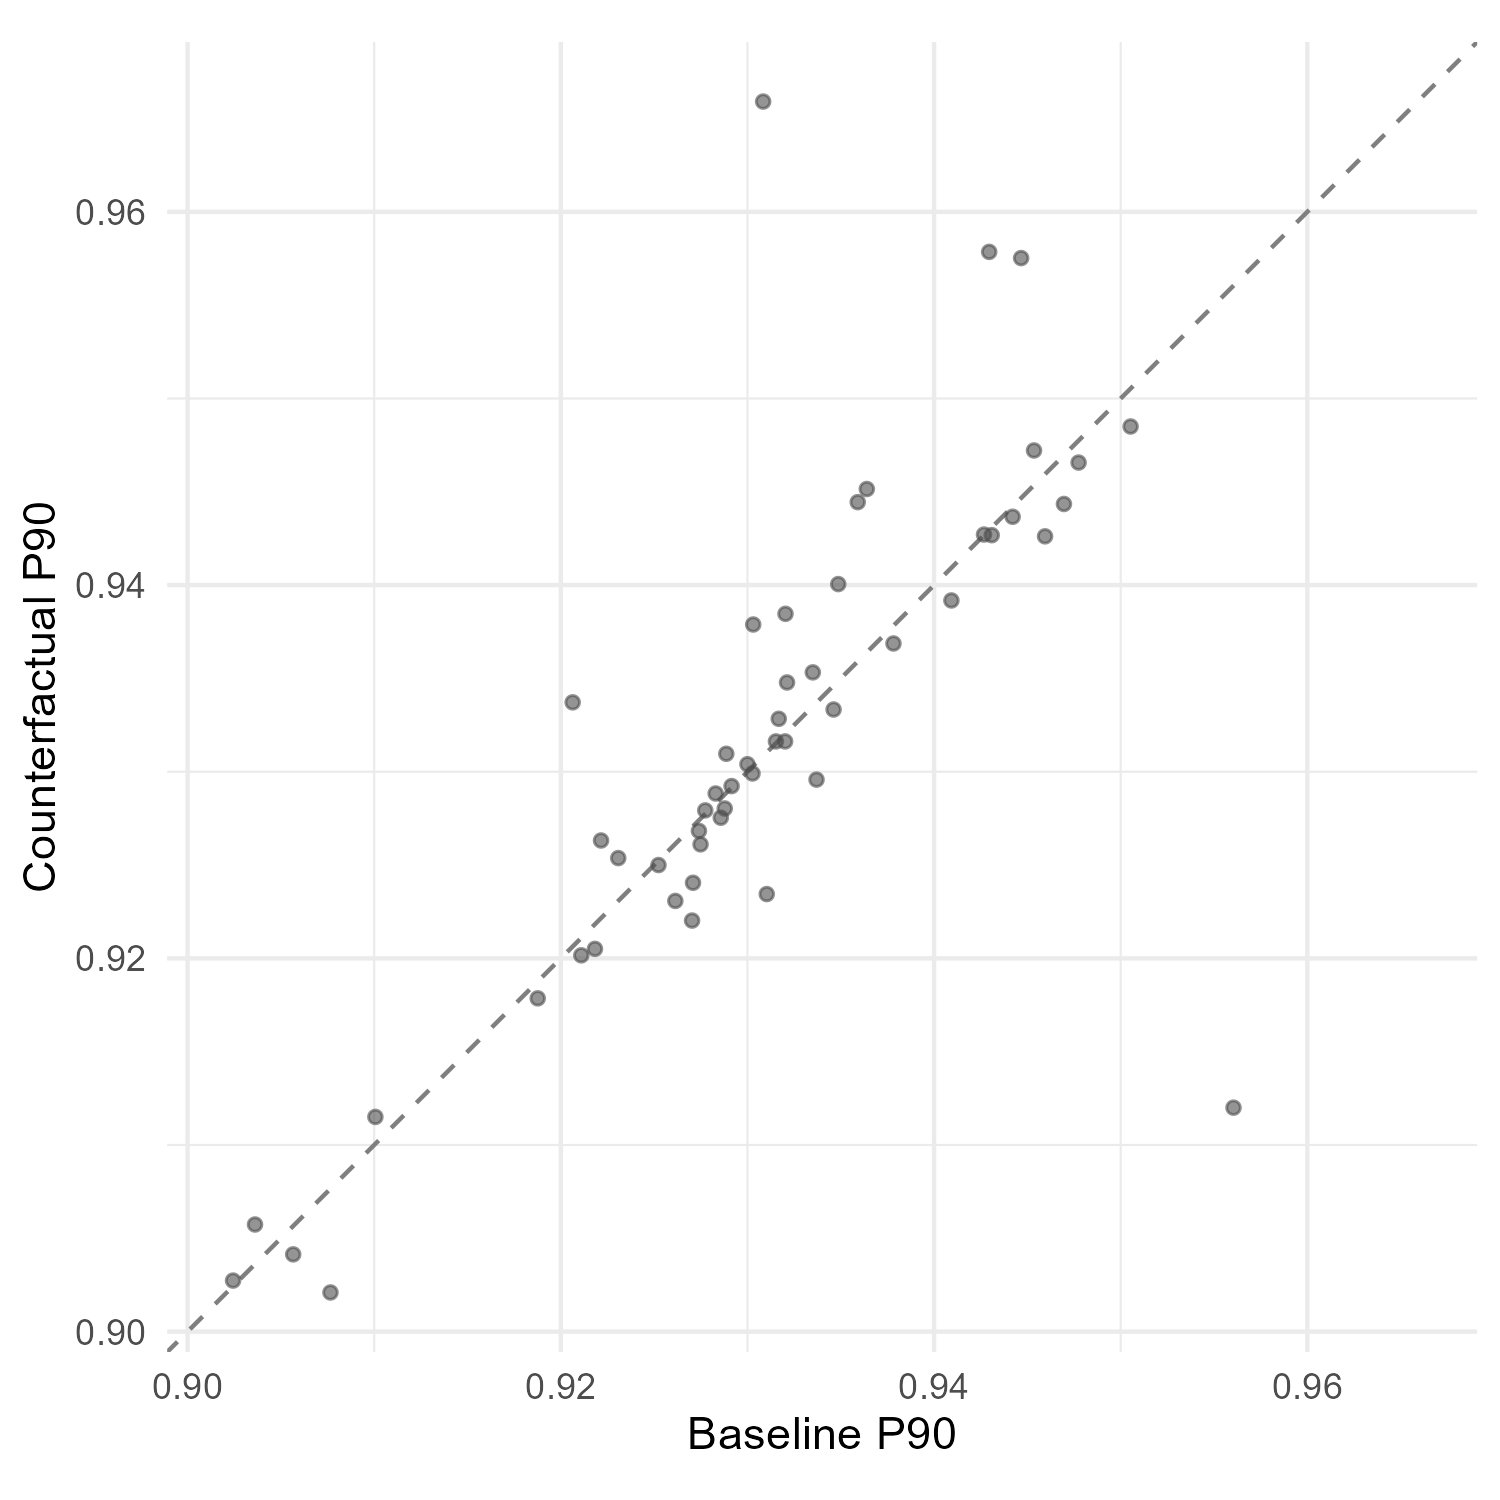
\includegraphics[height=2.2in,width=2.5in,keepaspectratio]{../../../results/figures/myopic-timevary/QualOffDiag_P90_current_Myopic_eta1.png} & 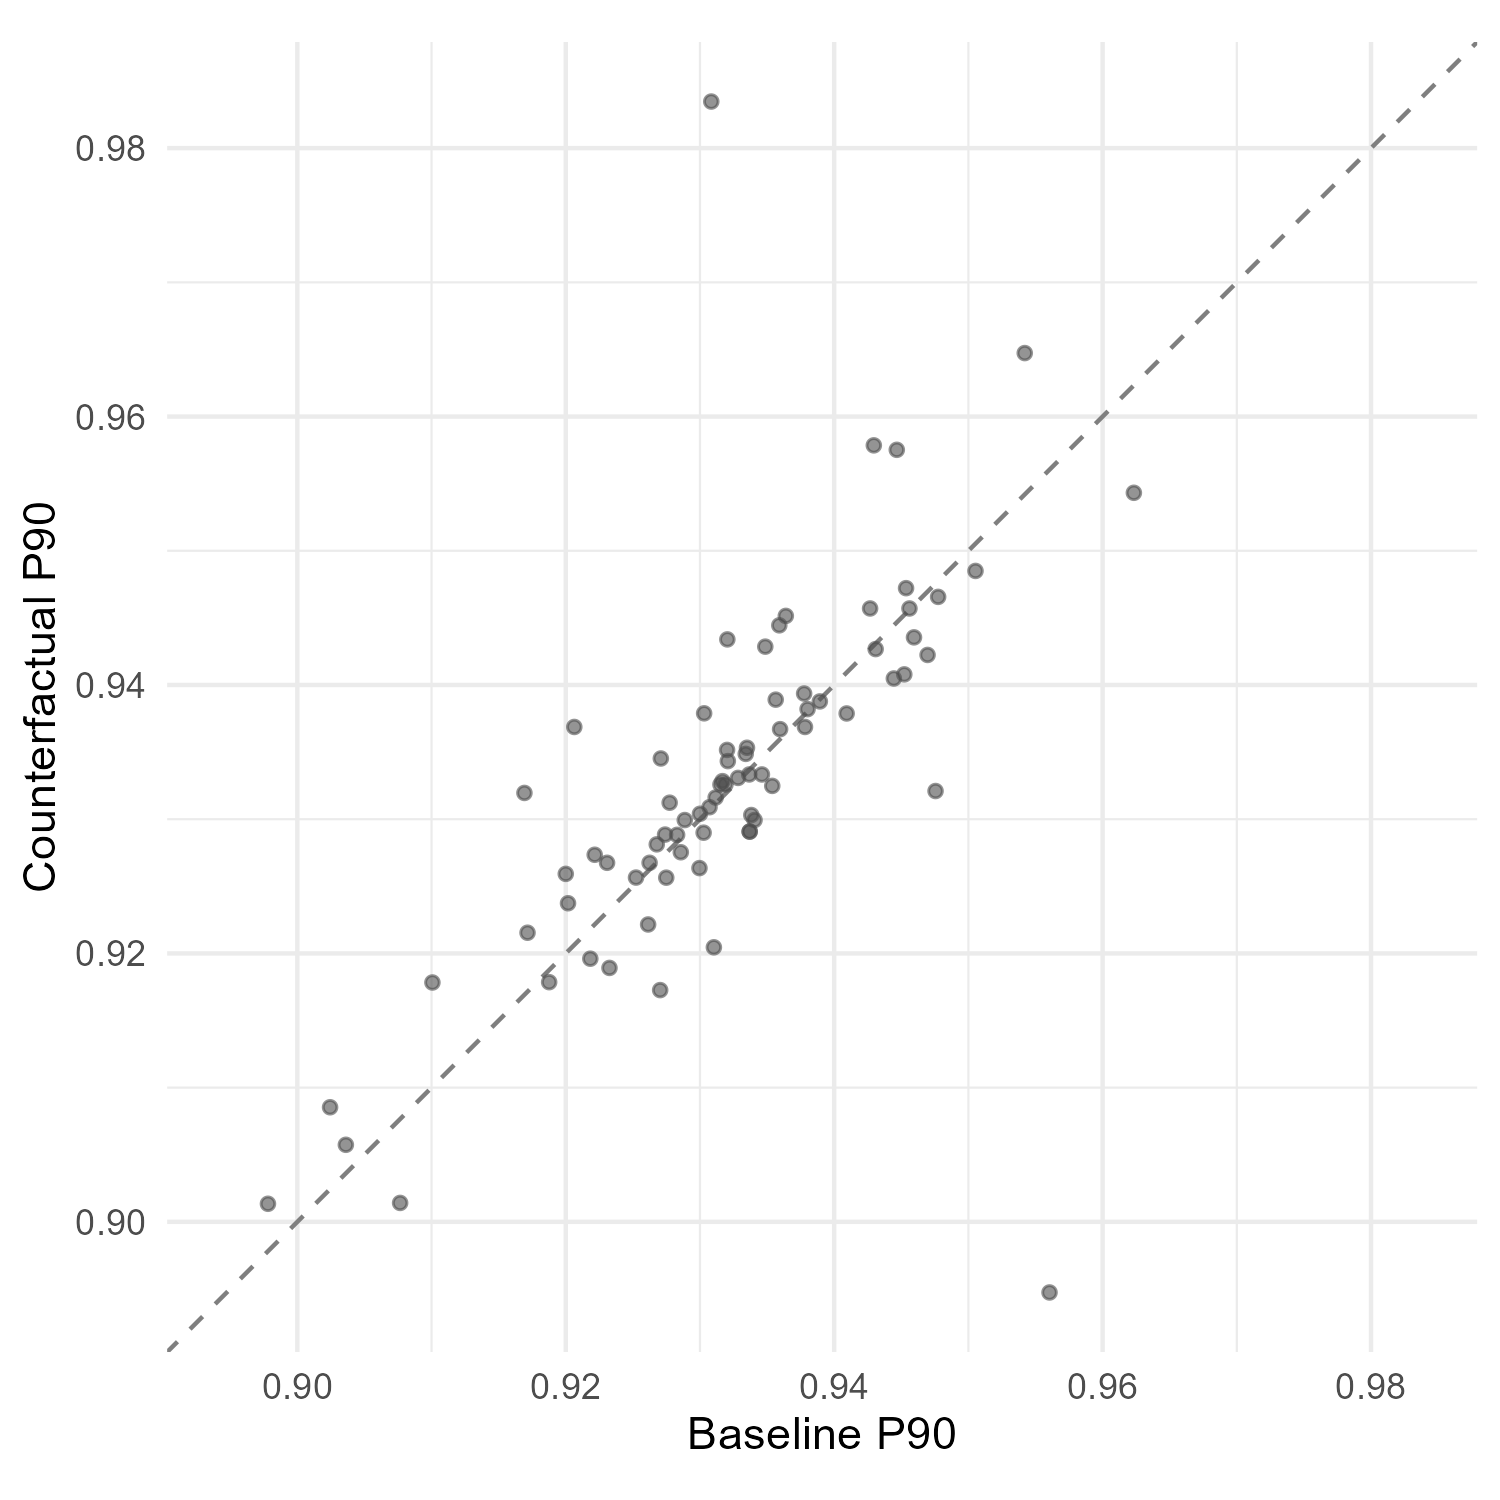
\includegraphics[height=2.2in,width=2.5in,keepaspectratio]{../../../results/figures/myopic-timevary/QualOffDiag_P90_full_Myopic_eta1.png} \\
\multicolumn{2}{c}{\textit{Forward-looking}} \\
Existing familiarity & Reset familiarity \\
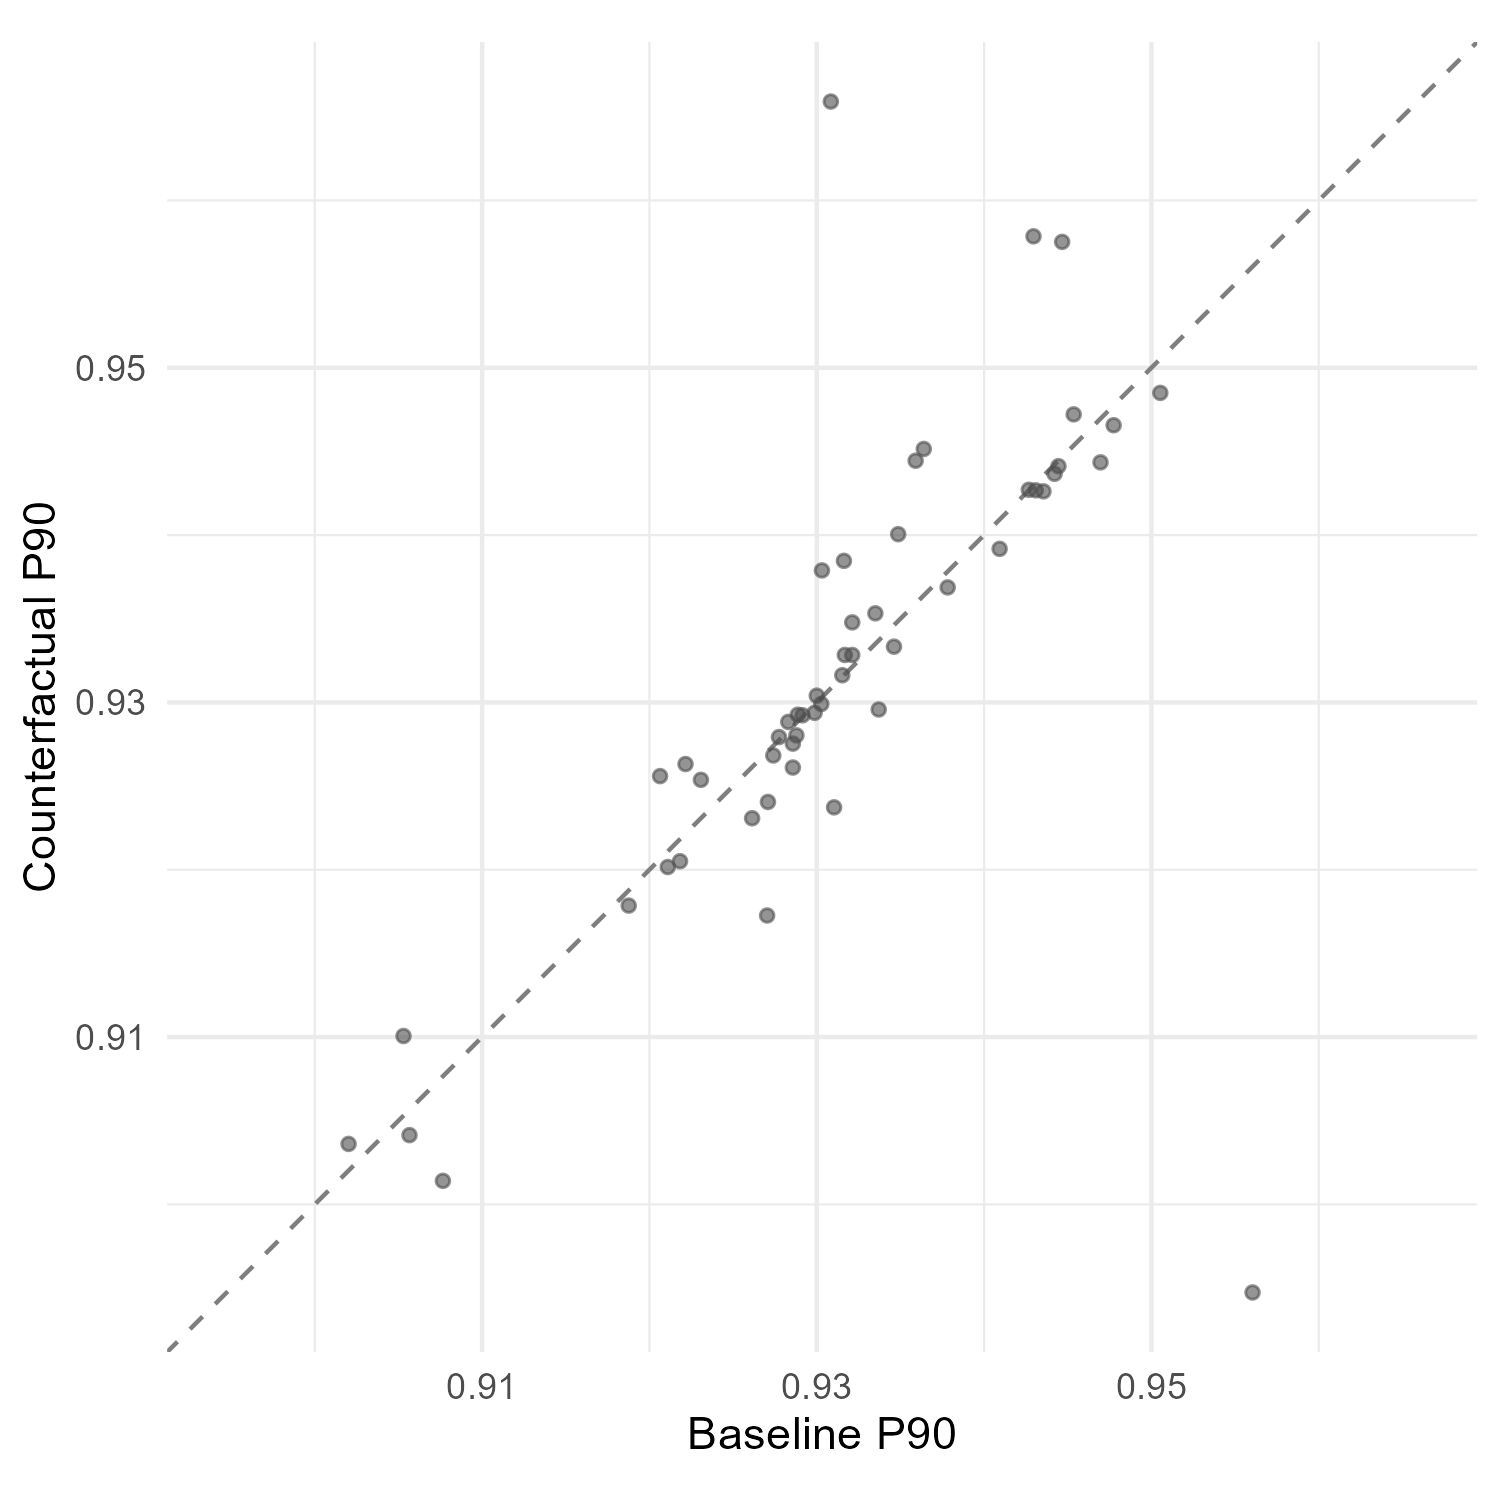
\includegraphics[height=2.2in,width=2.5in,keepaspectratio]{../../../results/figures/fwd-timevary/QualOffDiag_P90_current_FWD_eta1.png} & 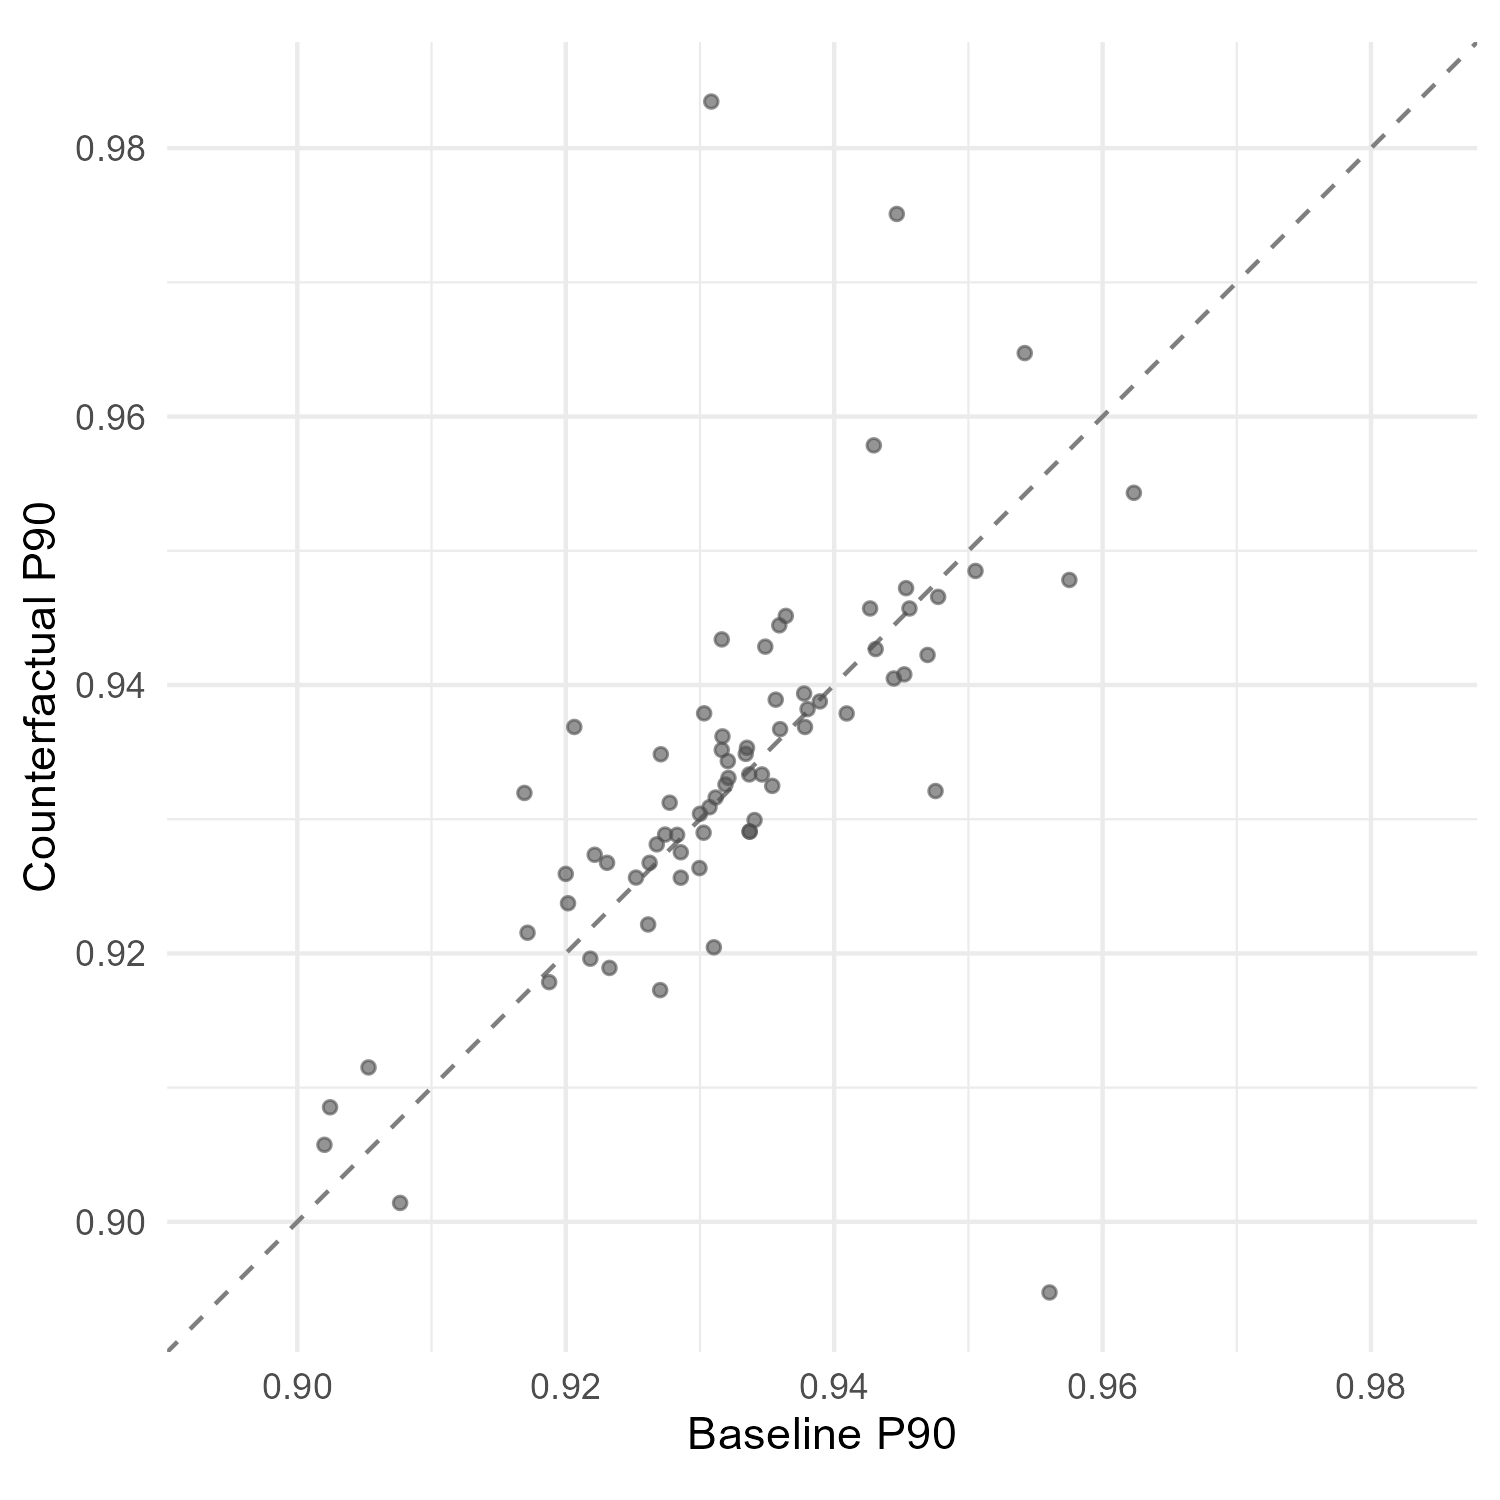
\includegraphics[height=2.2in,width=2.5in,keepaspectratio]{../../../results/figures/fwd-timevary/QualOffDiag_P90_full_FWD_eta1.png}
\end{tabular}
\label{fig:qualP90-cf}
\end{minipage}
\end{figure}

\clearpage
\begin{figure}[!ht]
\centering
\begin{minipage}[h]{6in}
\caption[SpendP10 Off-Diagonal]{Off-Diagonal Scatter of Patient-Weighted 10th-Percentile Spending ($\eta=1$)\footnote{Each point is an HRR where the patient-weighted 10th percentile of episode spending under the counterfactual differs from the baseline value. HRRs with identical baseline and counterfactual percentile are dropped (they lie on the 45-degree line). The solid reference line is the 45-degree line.}} %S: Typo in value of eta?
\centering
\begin{tabular}{cc}
\multicolumn{2}{c}{\textit{Myopic}} \\
Existing familiarity & Reset familiarity \\
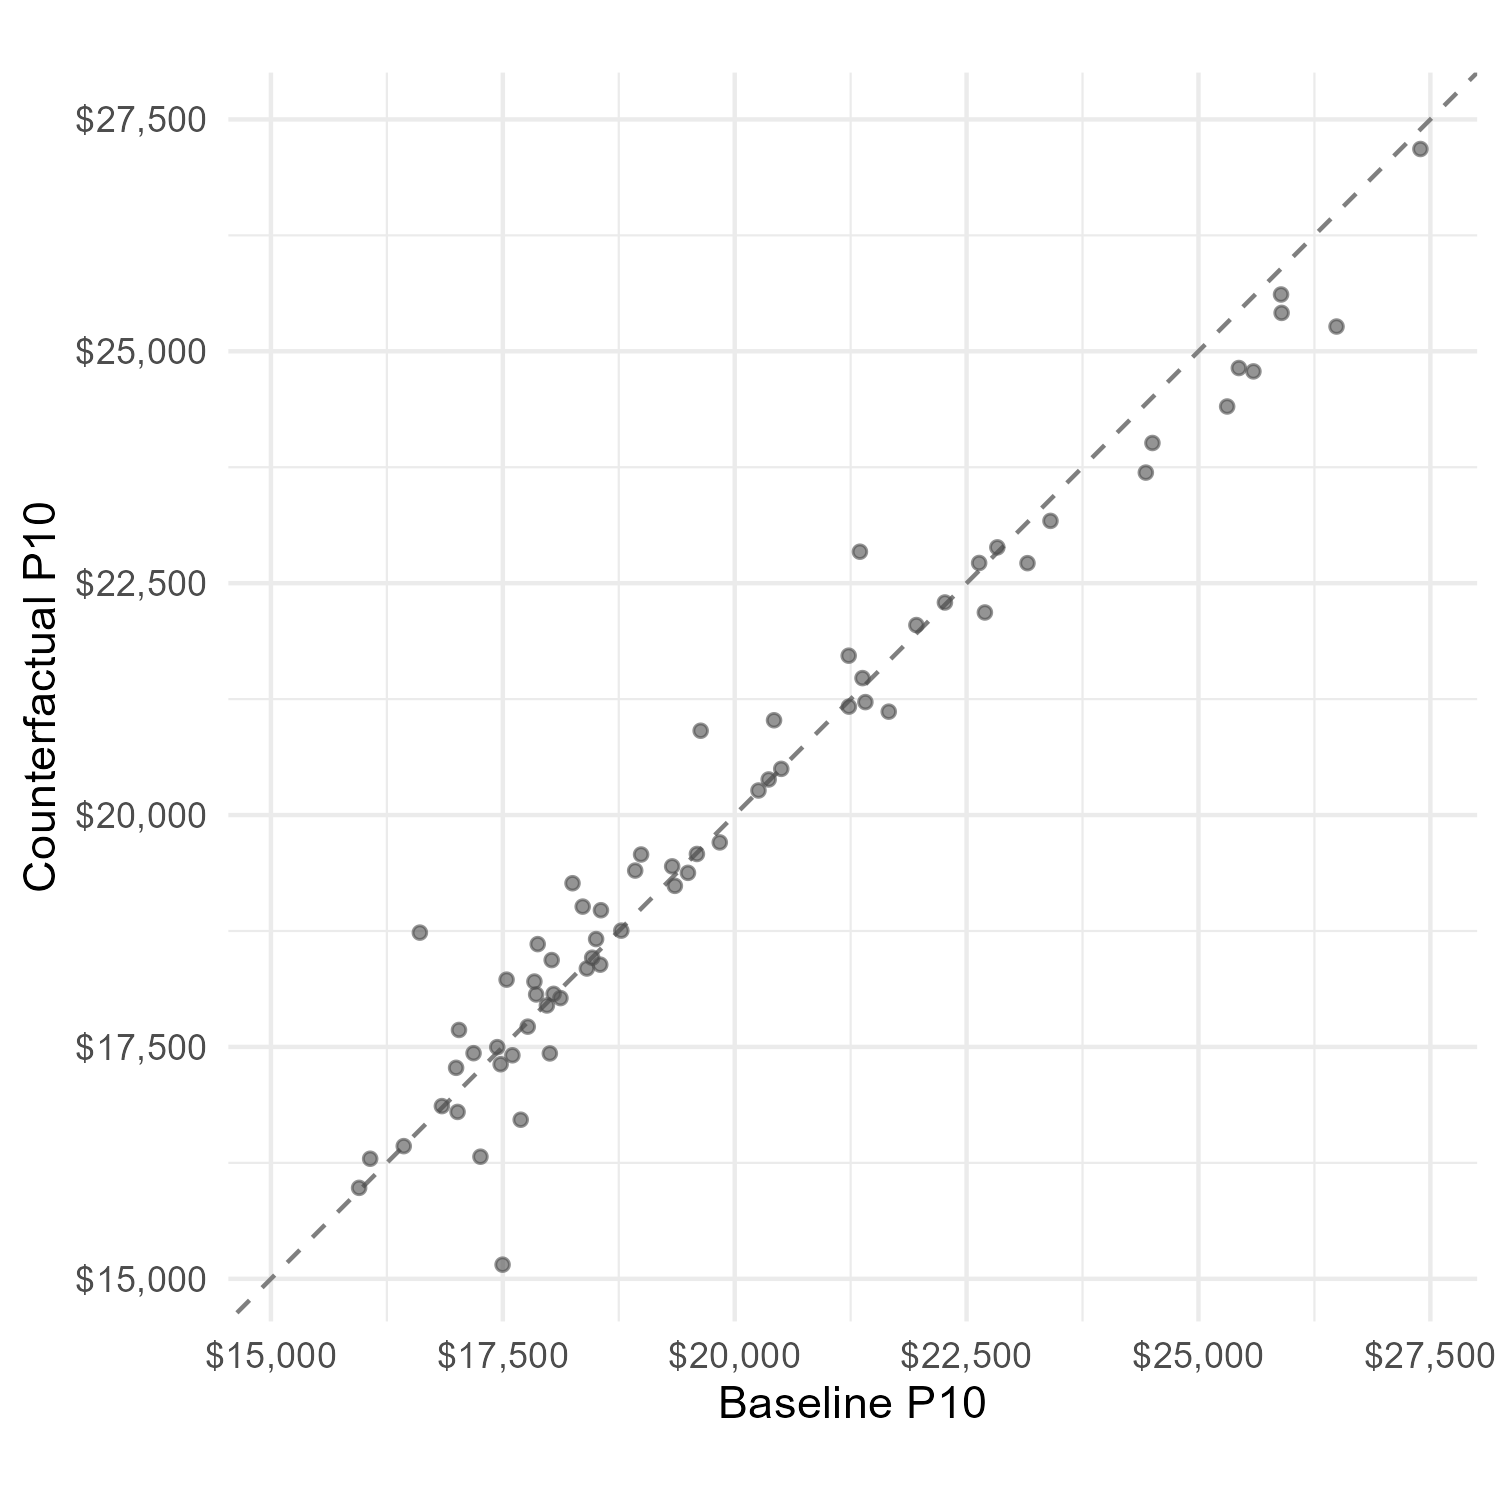
\includegraphics[height=2.2in,width=2.5in,keepaspectratio]{../../../results/figures/myopic-timevary/SpendOffDiag_P10_current_Myopic_eta1.png} & 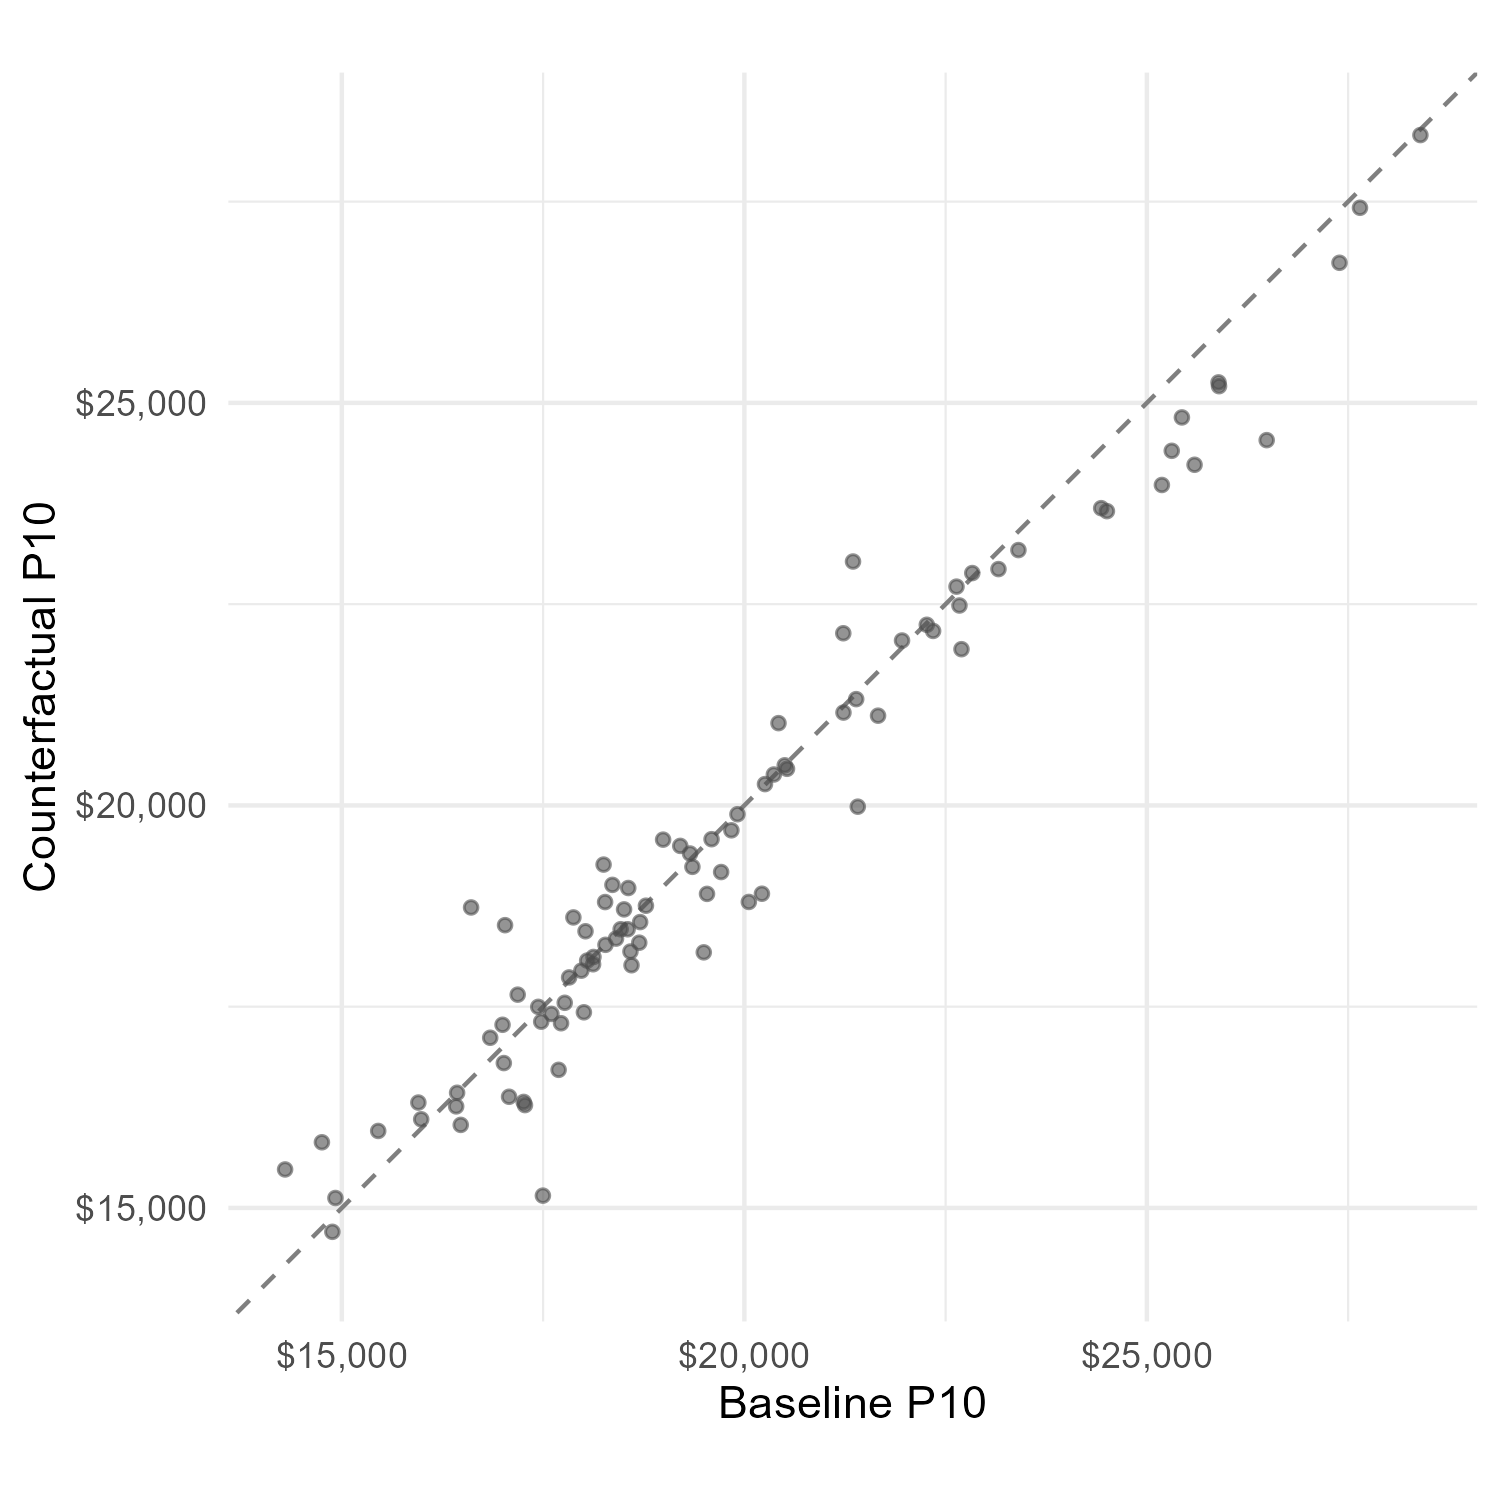
\includegraphics[height=2.2in,width=2.5in,keepaspectratio]{../../../results/figures/myopic-timevary/SpendOffDiag_P10_full_Myopic_eta1.png} \\
\multicolumn{2}{c}{\textit{Forward-looking}} \\
Existing familiarity & Reset familiarity \\
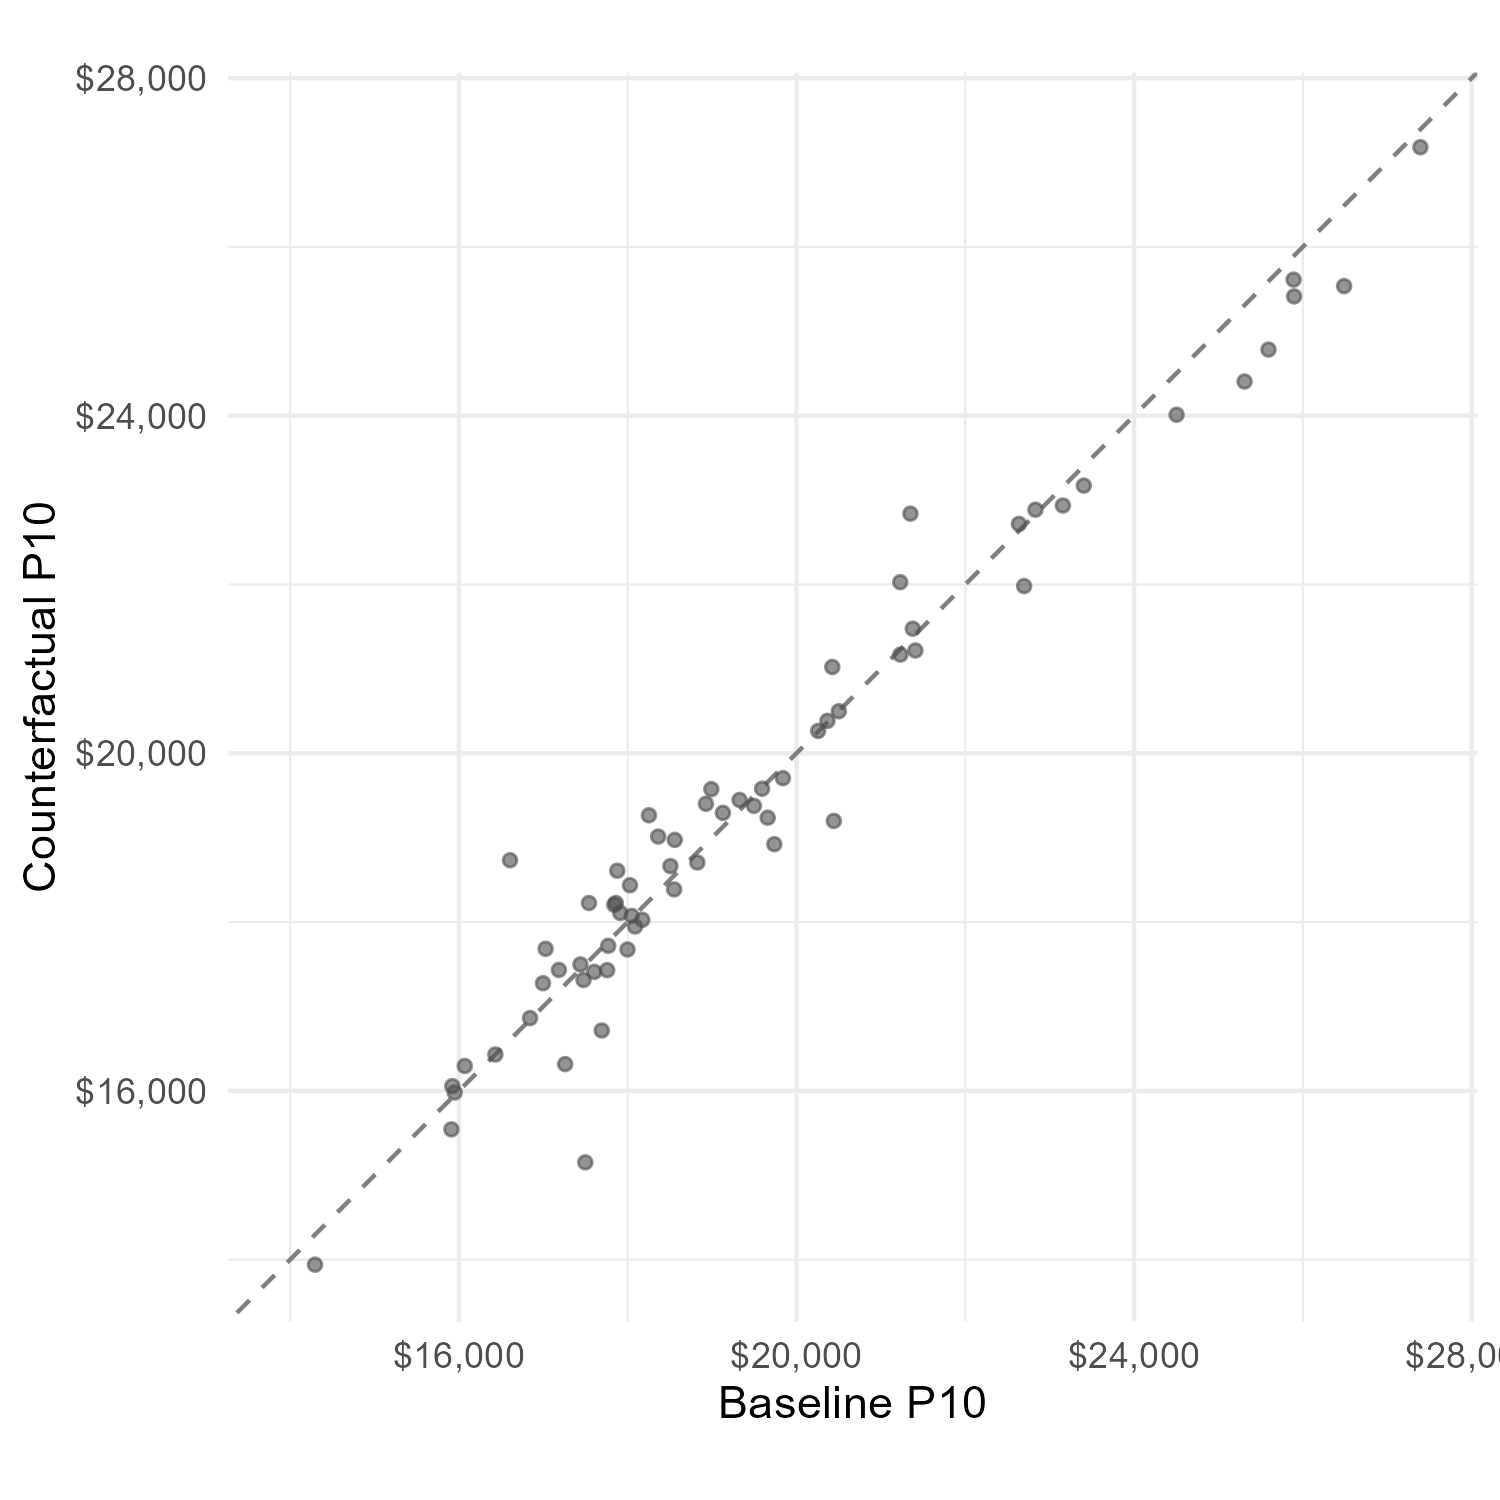
\includegraphics[height=2.2in,width=2.5in,keepaspectratio]{../../../results/figures/fwd-timevary/SpendOffDiag_P10_current_FWD_eta1.png} & 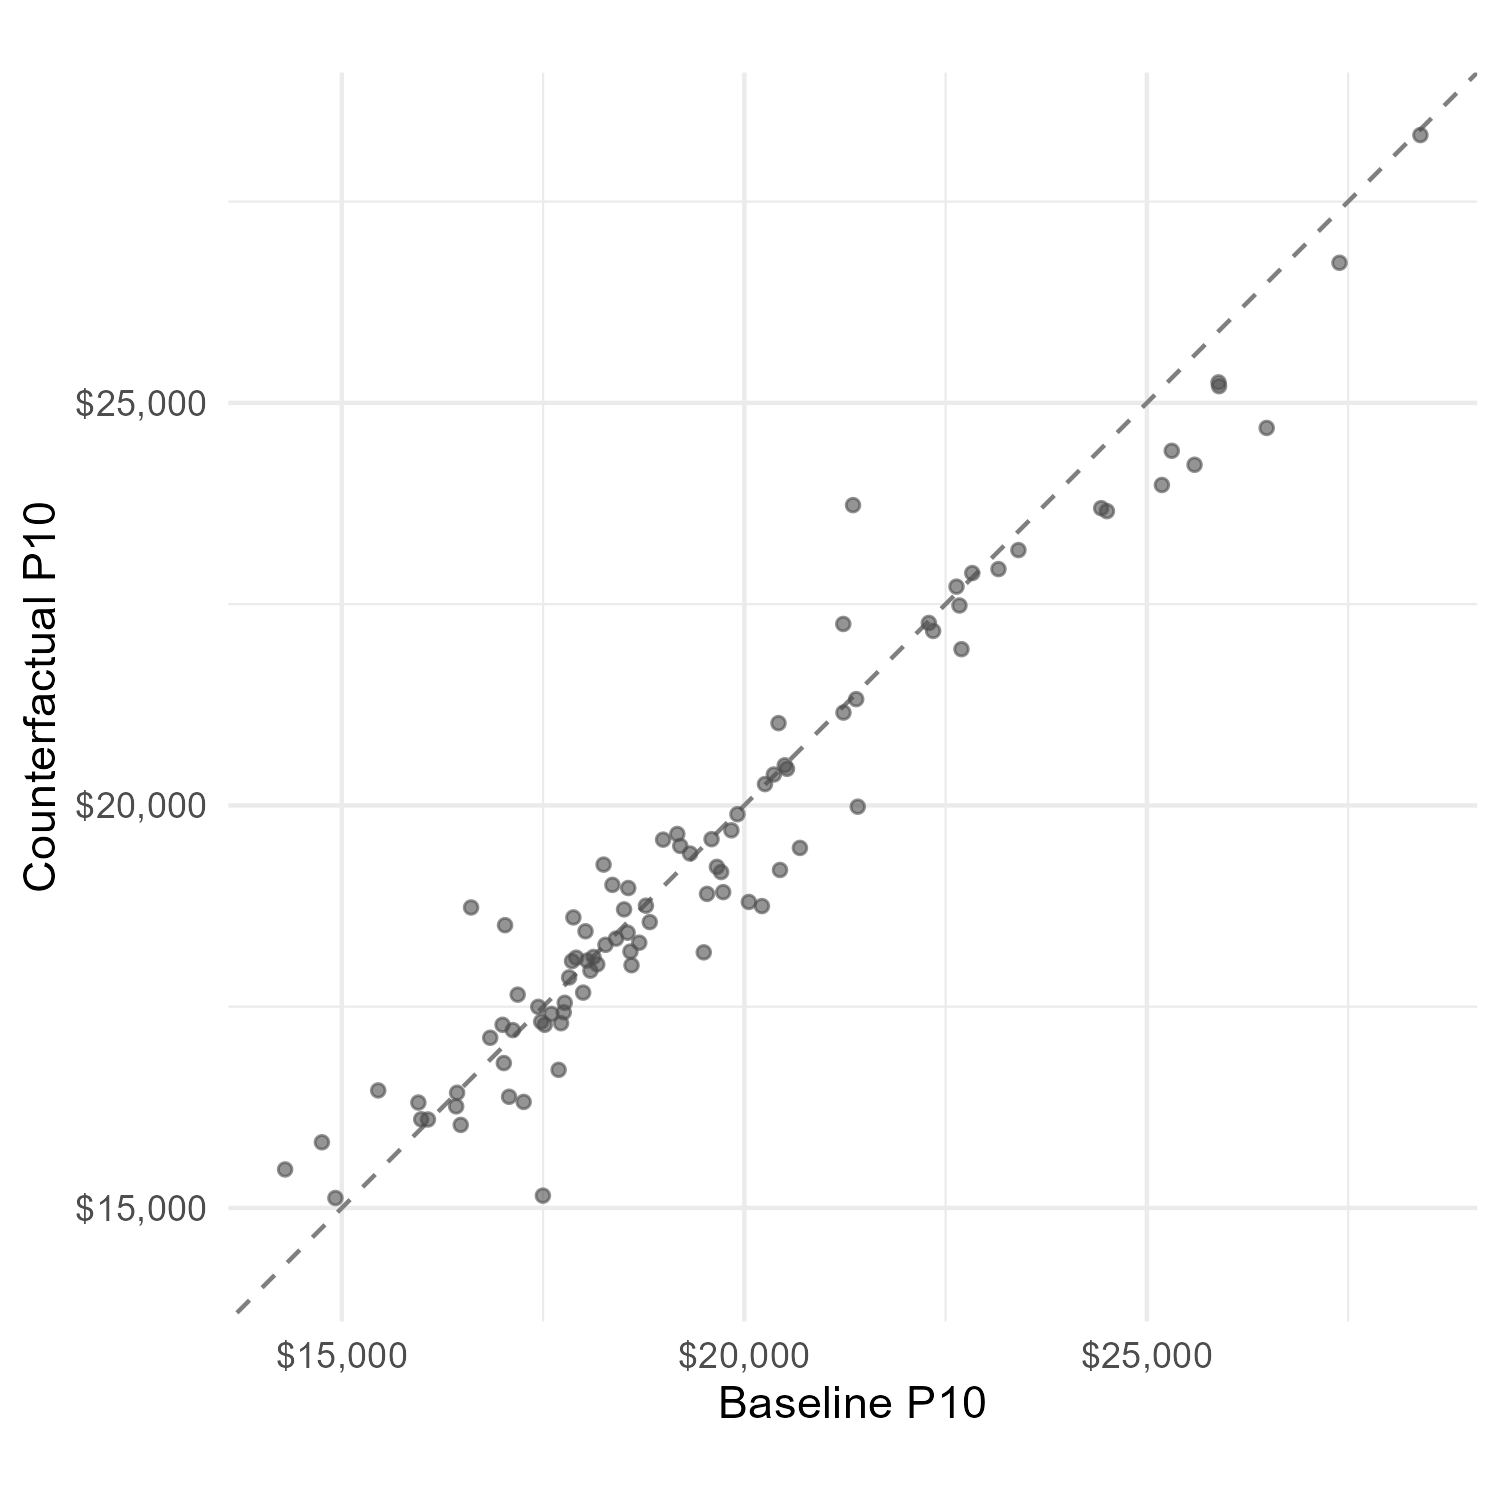
\includegraphics[height=2.2in,width=2.5in,keepaspectratio]{../../../results/figures/fwd-timevary/SpendOffDiag_P10_full_FWD_eta1.png}
\end{tabular}
\label{fig:spendP10-cf}
\end{minipage}
\end{figure}

\clearpage
\begin{figure}[!ht]
\centering
\begin{minipage}[h]{6in}
\caption[SpendP90 Off-Diagonal]{Off-Diagonal Scatter of Patient-Weighted 90th-Percentile Spending ($\eta=1$)\footnote{Each point is an HRR where the patient-weighted 90th percentile of episode spending under the counterfactual differs from the baseline value. HRRs with identical baseline and counterfactual percentile are dropped (they lie on the 45-degree line). The solid reference line is the 45-degree line.}} %S: Typo in value of eta?
\centering
\begin{tabular}{cc}
\multicolumn{2}{c}{\textit{Myopic}} \\
Existing familiarity & Reset familiarity \\
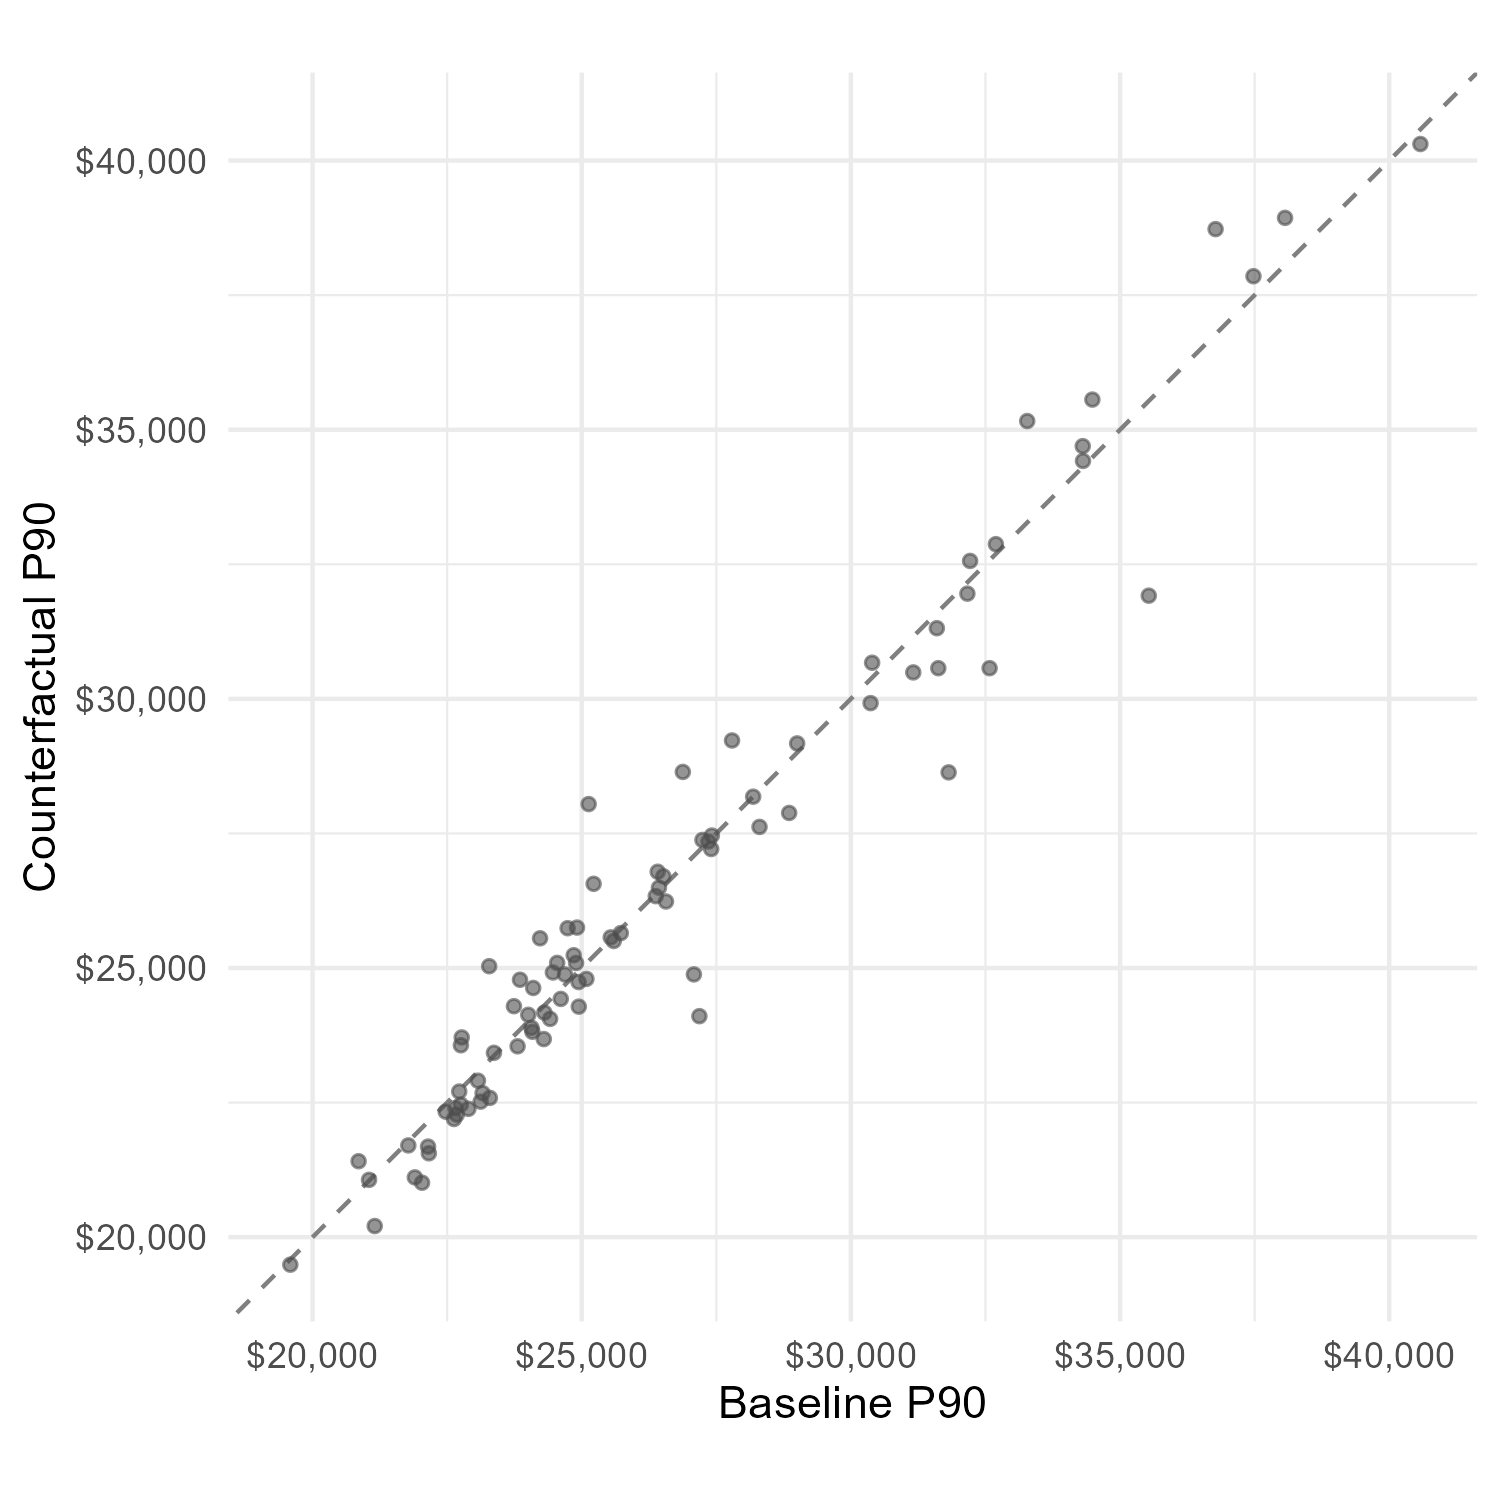
\includegraphics[height=2.2in,width=2.5in,keepaspectratio]{../../../results/figures/myopic-timevary/SpendOffDiag_P90_current_Myopic_eta1.png} & 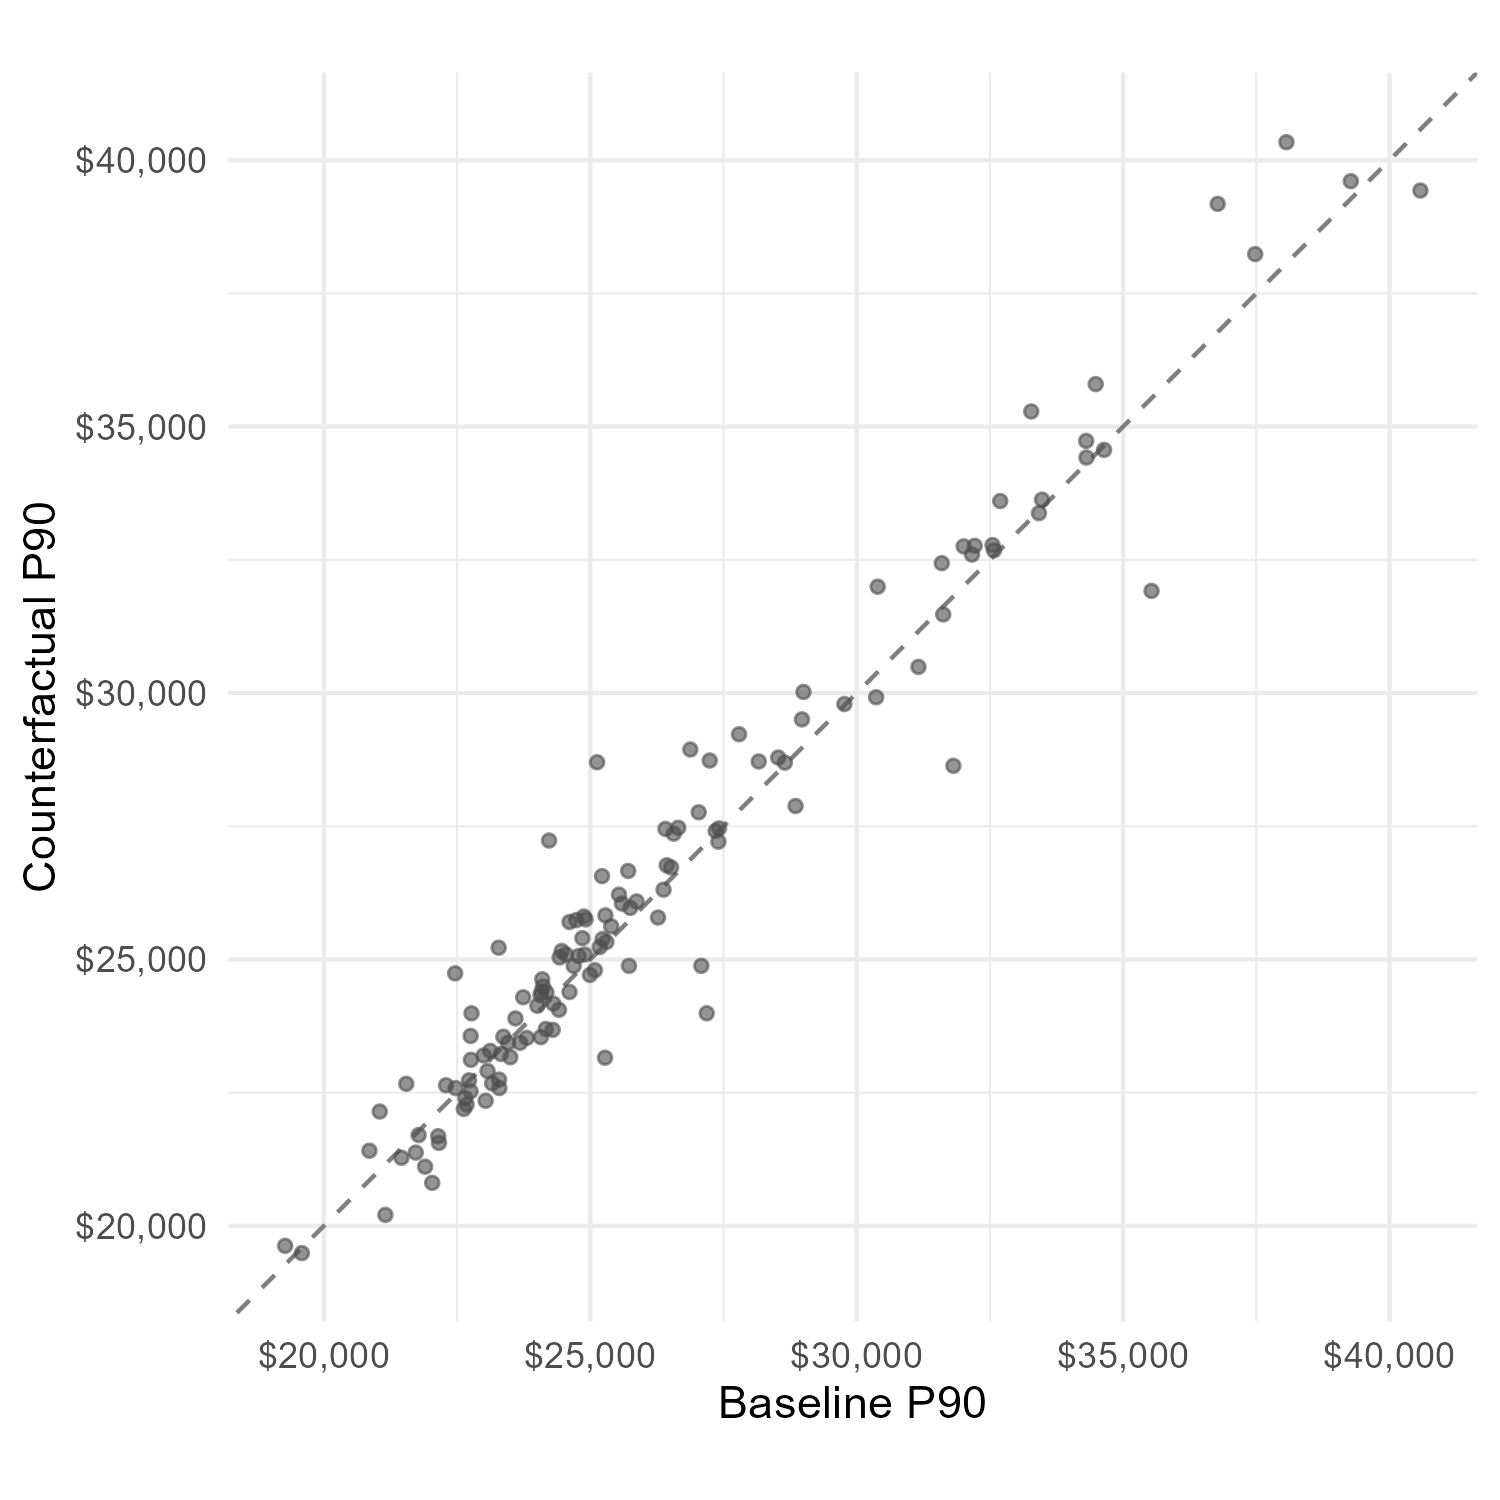
\includegraphics[height=2.2in,width=2.5in,keepaspectratio]{../../../results/figures/myopic-timevary/SpendOffDiag_P90_full_Myopic_eta1.png} \\
\multicolumn{2}{c}{\textit{Forward-looking}} \\
Existing familiarity & Reset familiarity \\
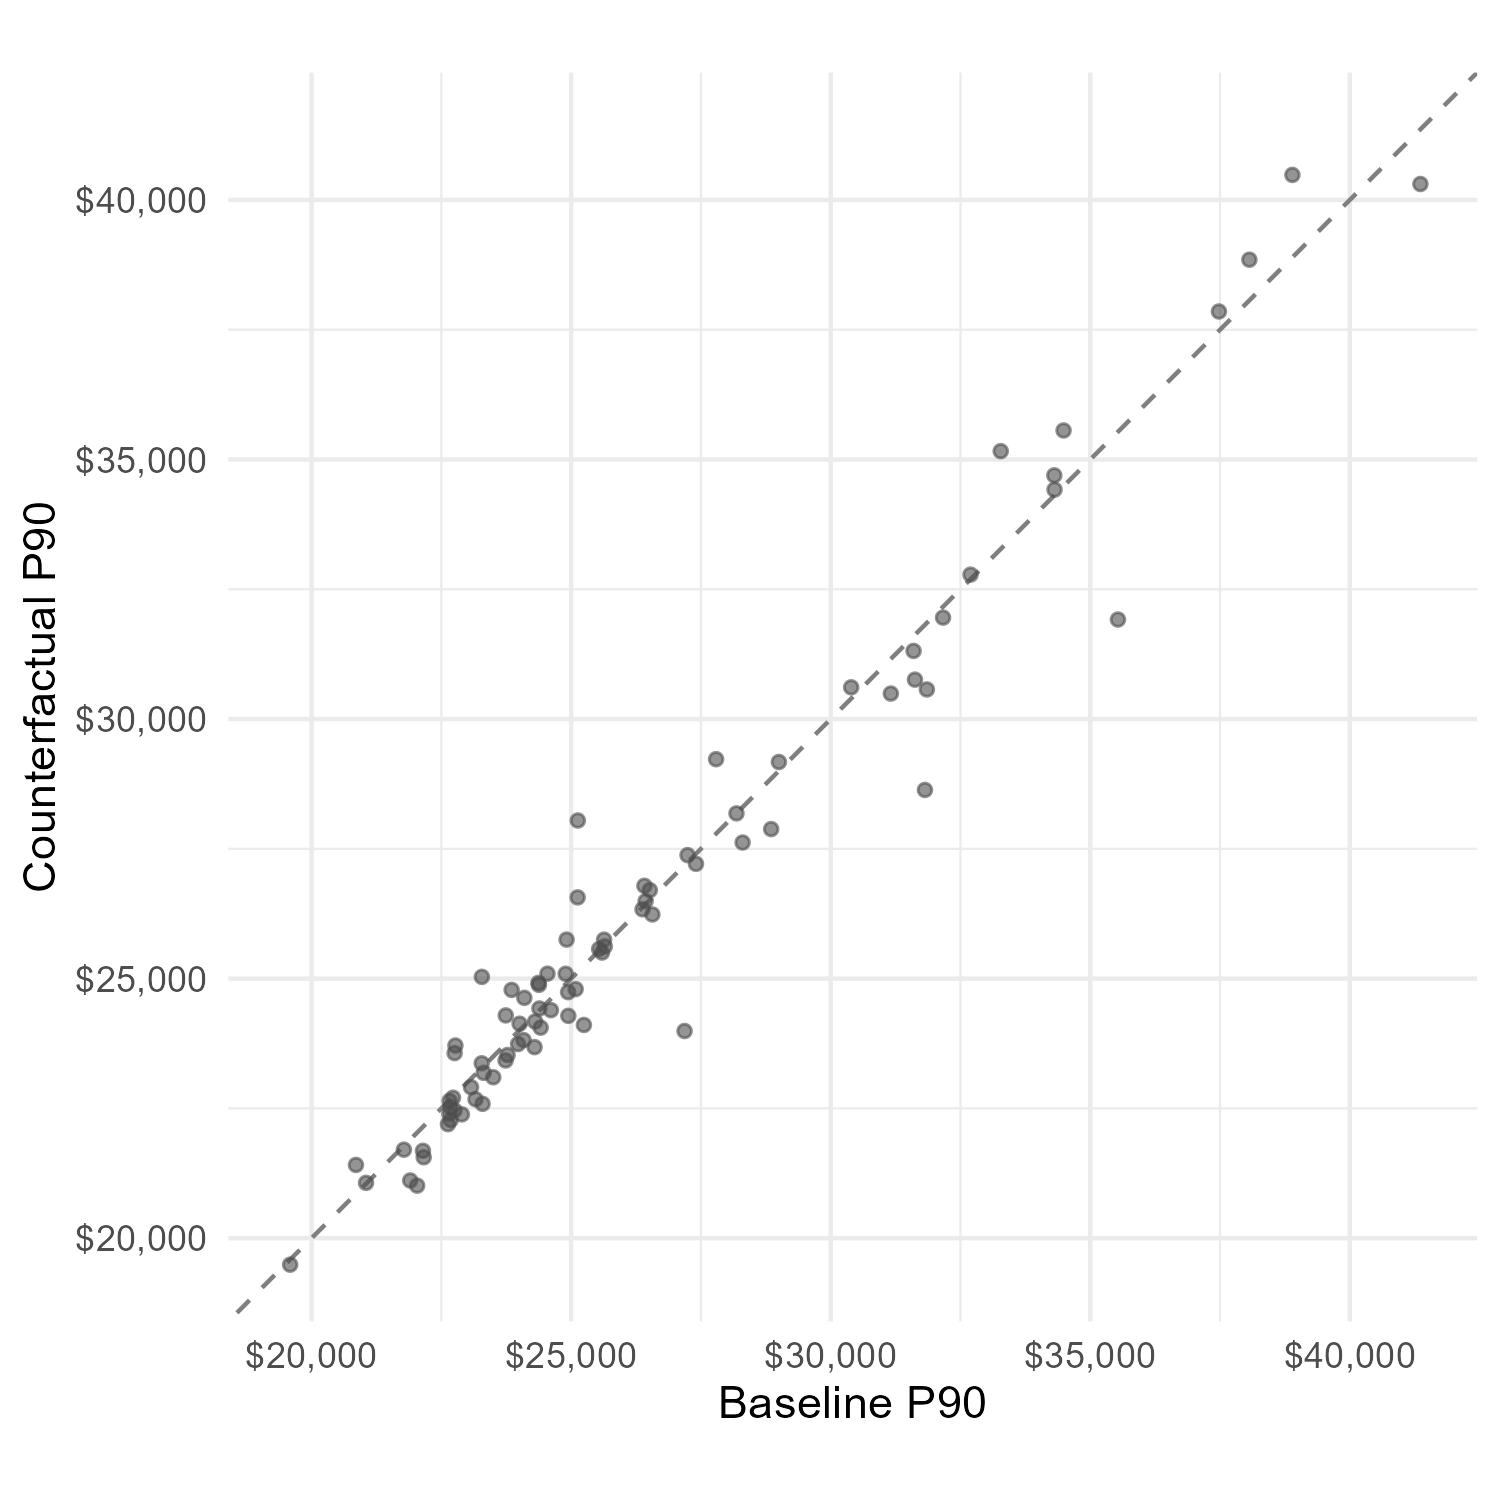
\includegraphics[height=2.2in,width=2.5in,keepaspectratio]{../../../results/figures/fwd-timevary/SpendOffDiag_P90_current_FWD_eta1.png} & 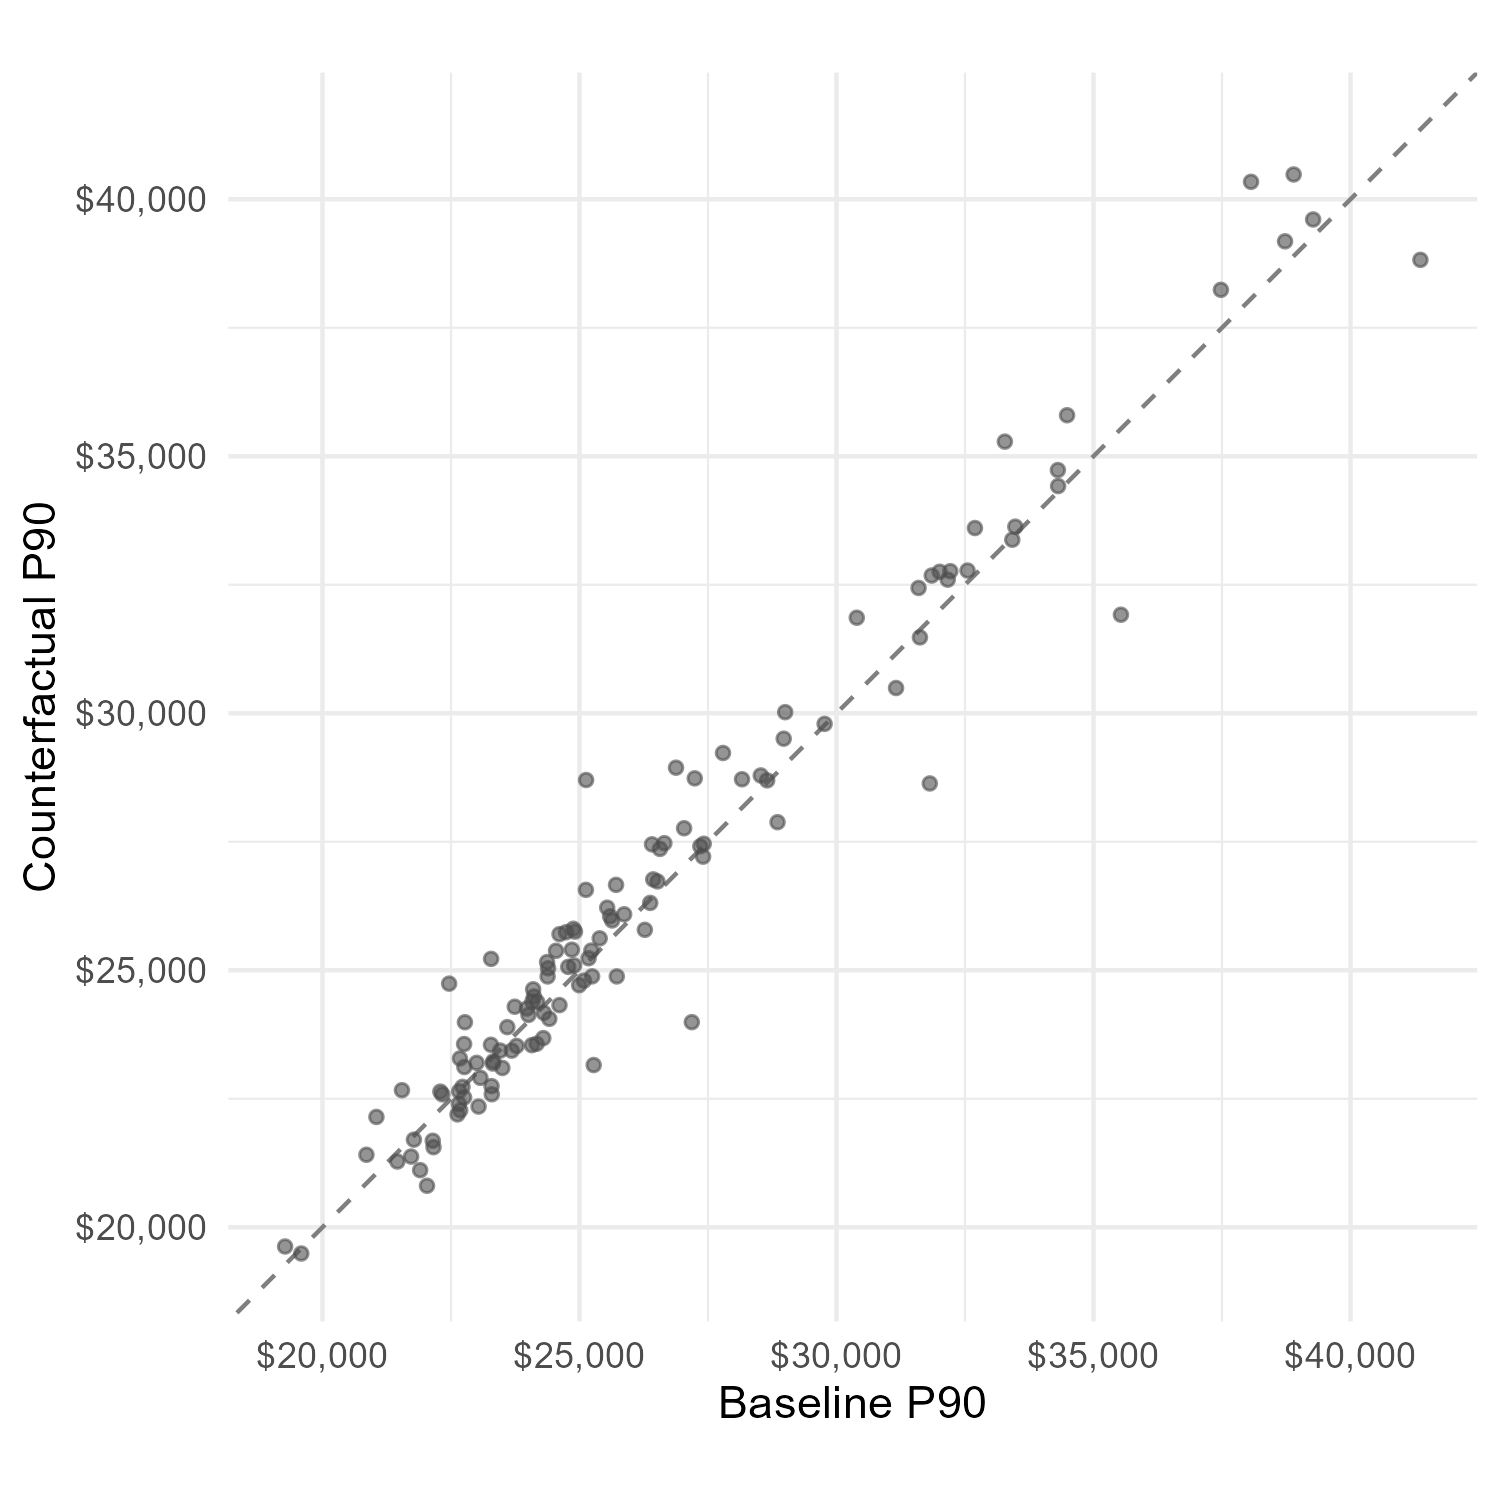
\includegraphics[height=2.2in,width=2.5in,keepaspectratio]{../../../results/figures/fwd-timevary/SpendOffDiag_P90_full_FWD_eta1.png}
\end{tabular}
\label{fig:spendP90-cf}
\end{minipage}
\end{figure}


%%% F. ADDITIONAL FIGURES

\clearpage
\section*{Additional Figures}

This section presents corresponding figures for $\eta=5$ of the counterfactual gradients and off-diagonal percentile scatters shown elsewhere in the paper and appendix for $\eta=1$.

\begin{figure}[!h]
\centering
\begin{minipage}[h]{6in}
\caption[Gradient of Health Effects ($\eta=5$)]{Health Effects of Full Information by Estimated Learning Parameter ($\eta=5$)\footnote{Figure depicts the mean change in successes per 10,000 patients under each counterfactual, binned into ten patient-weighted quantiles of the estimated learning parameter $\hat\alpha$ within each HRR ($\hat\alpha > 0.001$). Marker size reflects the total patients in the bin.}}
\centering
\begin{tabular}{cc}
\multicolumn{2}{c}{\textit{Myopic}} \\
Existing familiarity & Reset familiarity \\
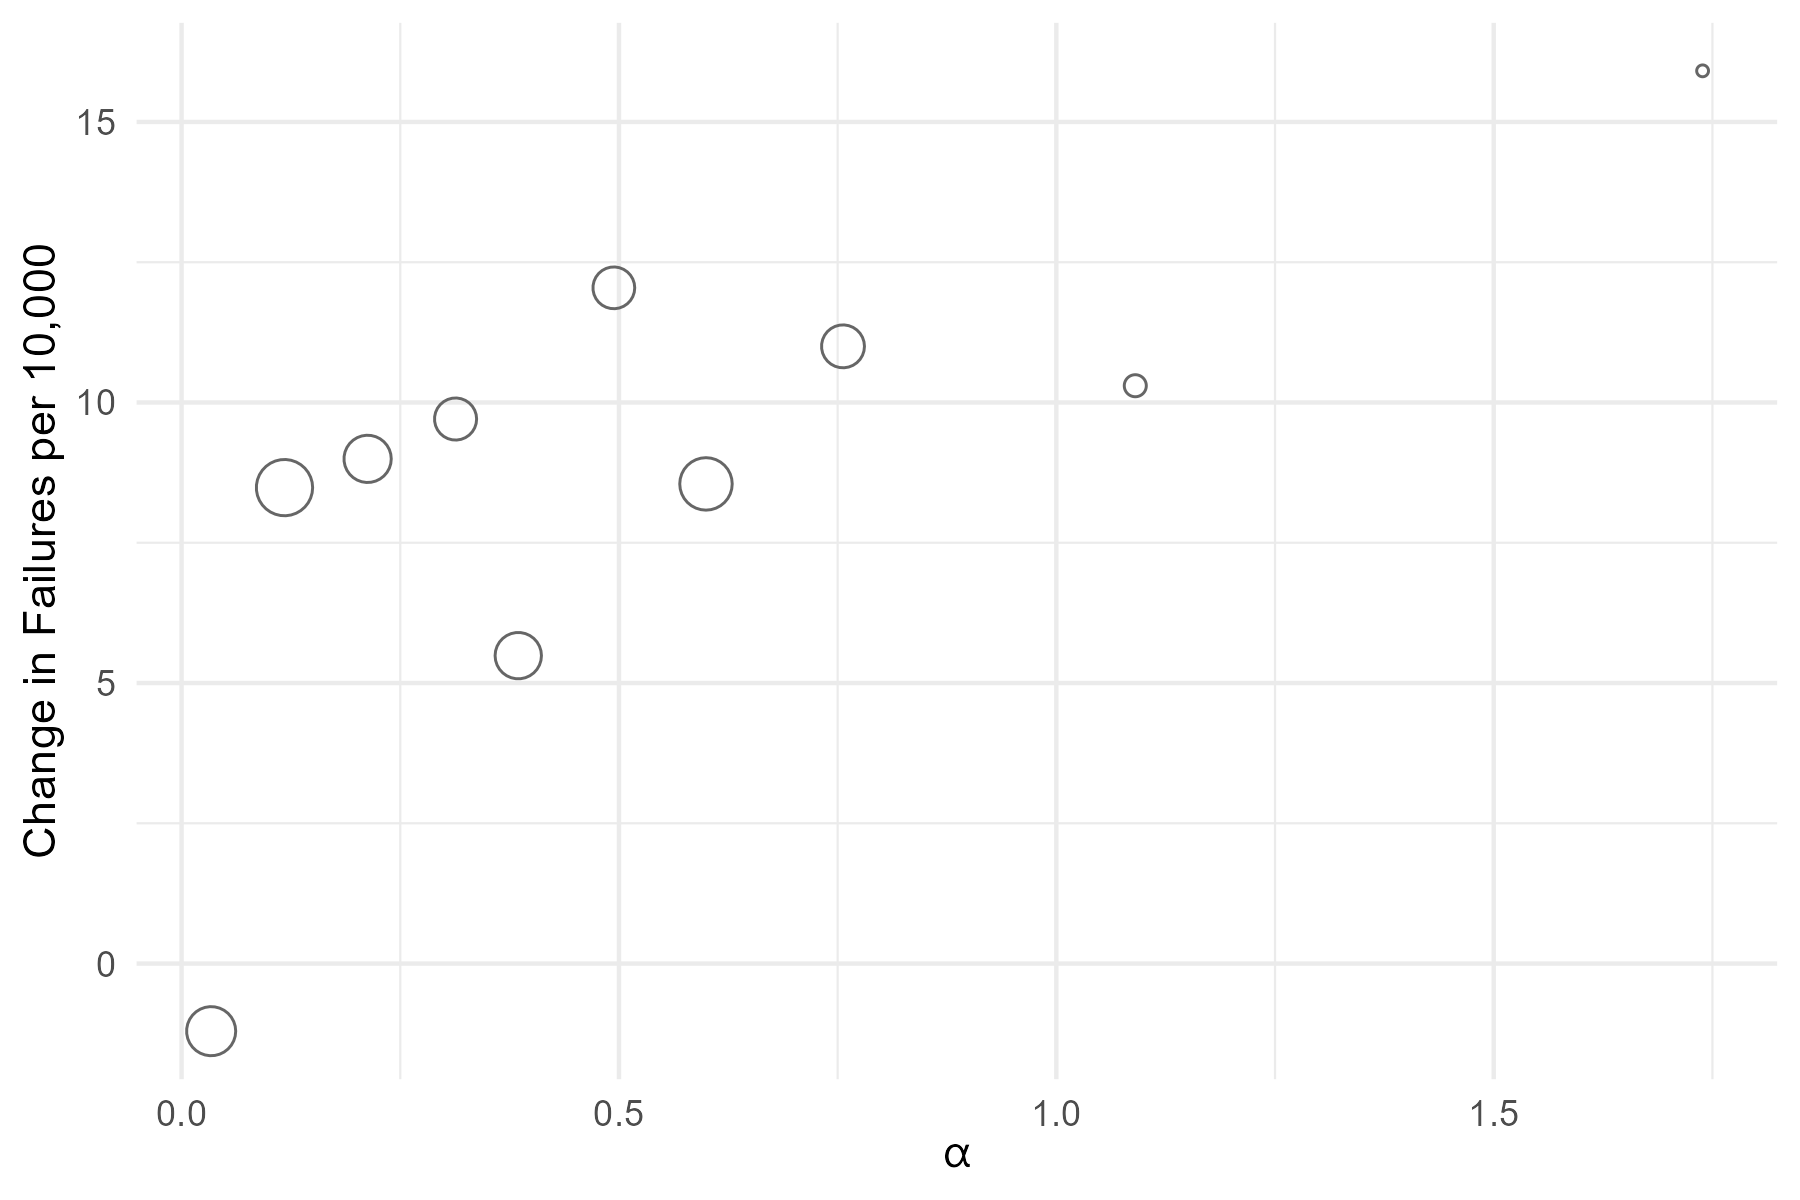
\includegraphics[height=1.6in,width=2.7in,keepaspectratio]{../../../results/figures/myopic-timevary/Gradient_HealthFX_current_Myopic_eta5.png} & \includegraphics[height=1.6in,width=2.7in,keepaspectratio]{../../../results/figures/myopic-timevary/Gradient_HealthFX_full_Myopic_eta5.png} \\
\multicolumn{2}{c}{\textit{Forward-looking}} \\
Existing familiarity & Reset familiarity \\
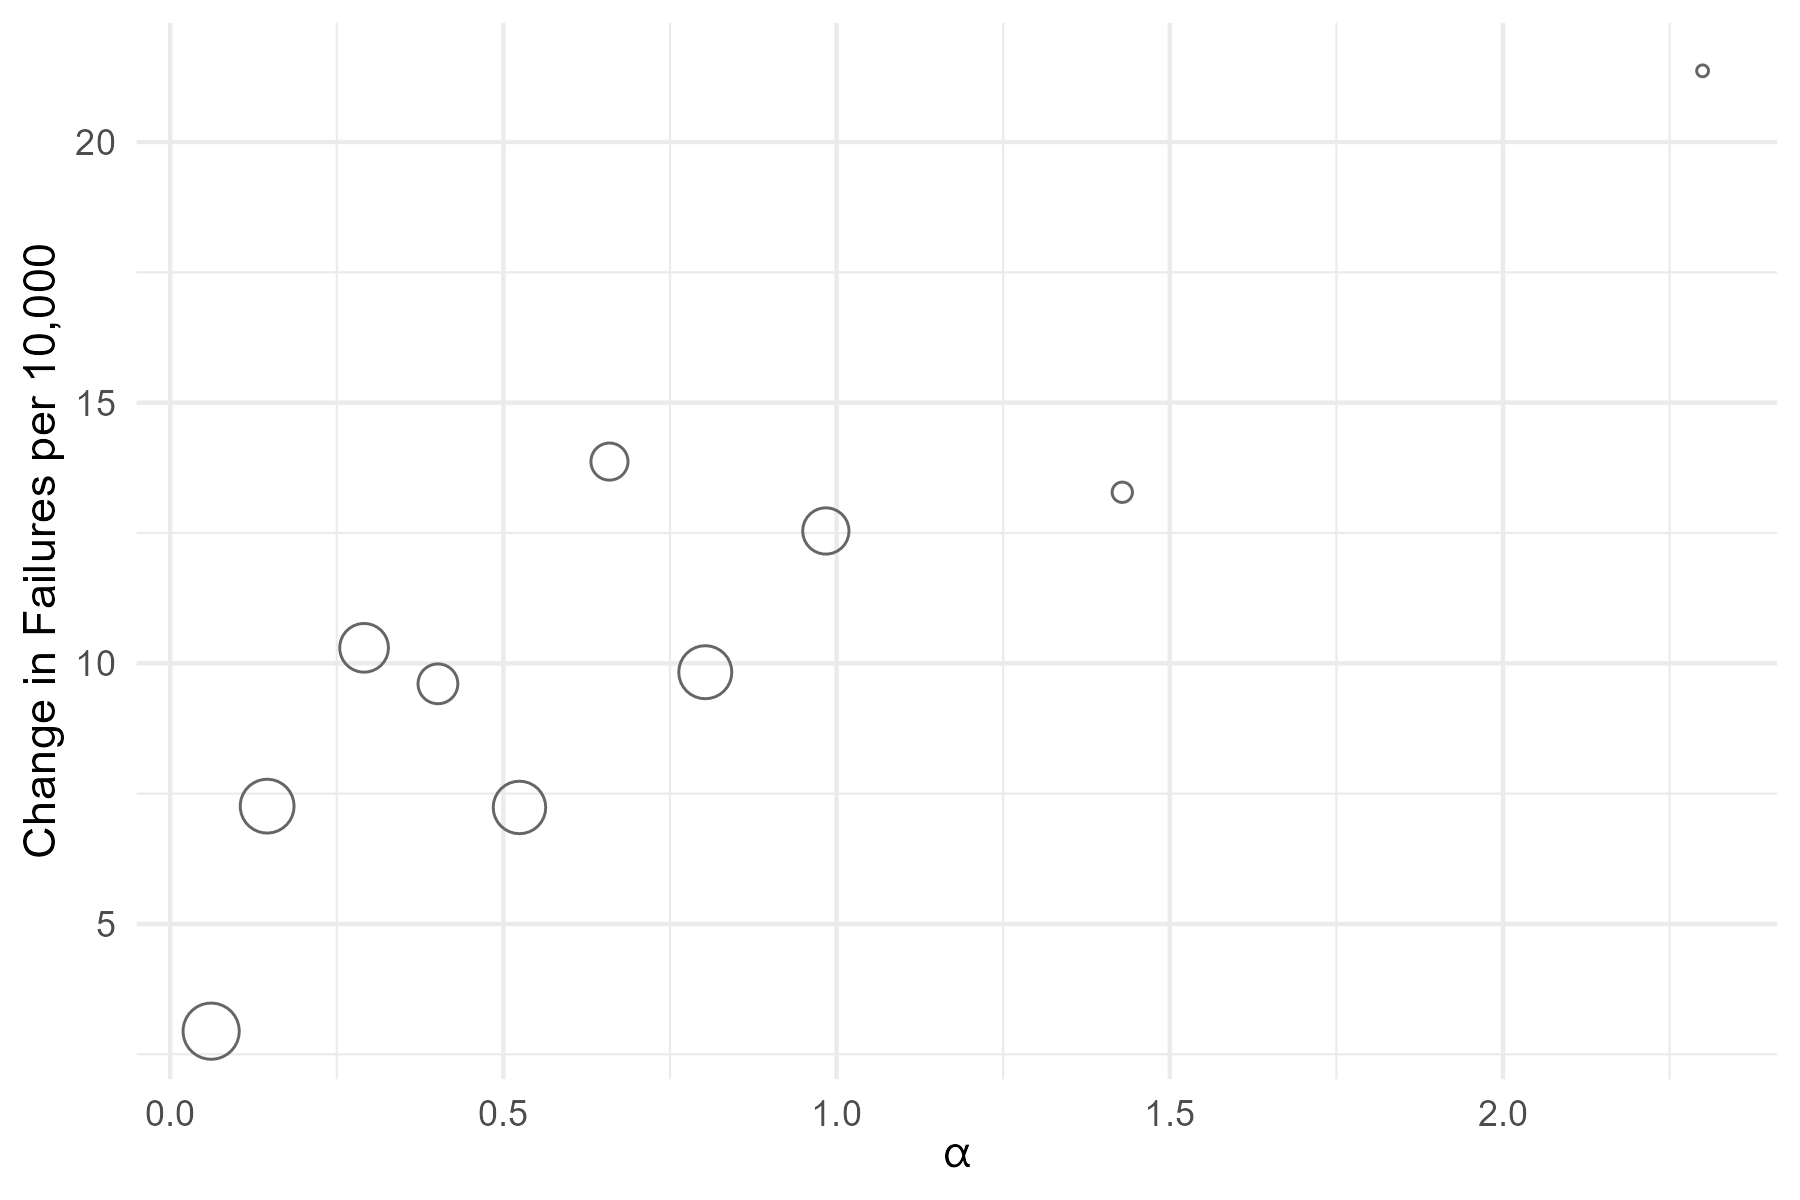
\includegraphics[height=1.6in,width=2.7in,keepaspectratio]{../../../results/figures/fwd-timevary/Gradient_HealthFX_current_FWD_eta5.png} & \includegraphics[height=1.6in,width=2.7in,keepaspectratio]{../../../results/figures/fwd-timevary/Gradient_HealthFX_full_FWD_eta5.png}
\end{tabular}
\label{fig:gradient_health_eta5}
\end{minipage}
\end{figure}

\clearpage
\begin{figure}[!ht]
\centering
\begin{minipage}[h]{6in}
\caption[Gradient of Spending Effects ($\eta=5$)]{Episode Spending Effects of Full Information by Estimated Learning Parameter ($\eta=5$)\footnote{Figure depicts the mean change in episode spending under each counterfactual, binned into ten patient-weighted quantiles of the estimated learning parameter $\hat\alpha$ within each HRR ($\hat\alpha > 0.001$). Marker size reflects the total patients in the bin.}}
\centering
\begin{tabular}{cc}
\multicolumn{2}{c}{\textit{Myopic}} \\
Existing familiarity & Reset familiarity \\
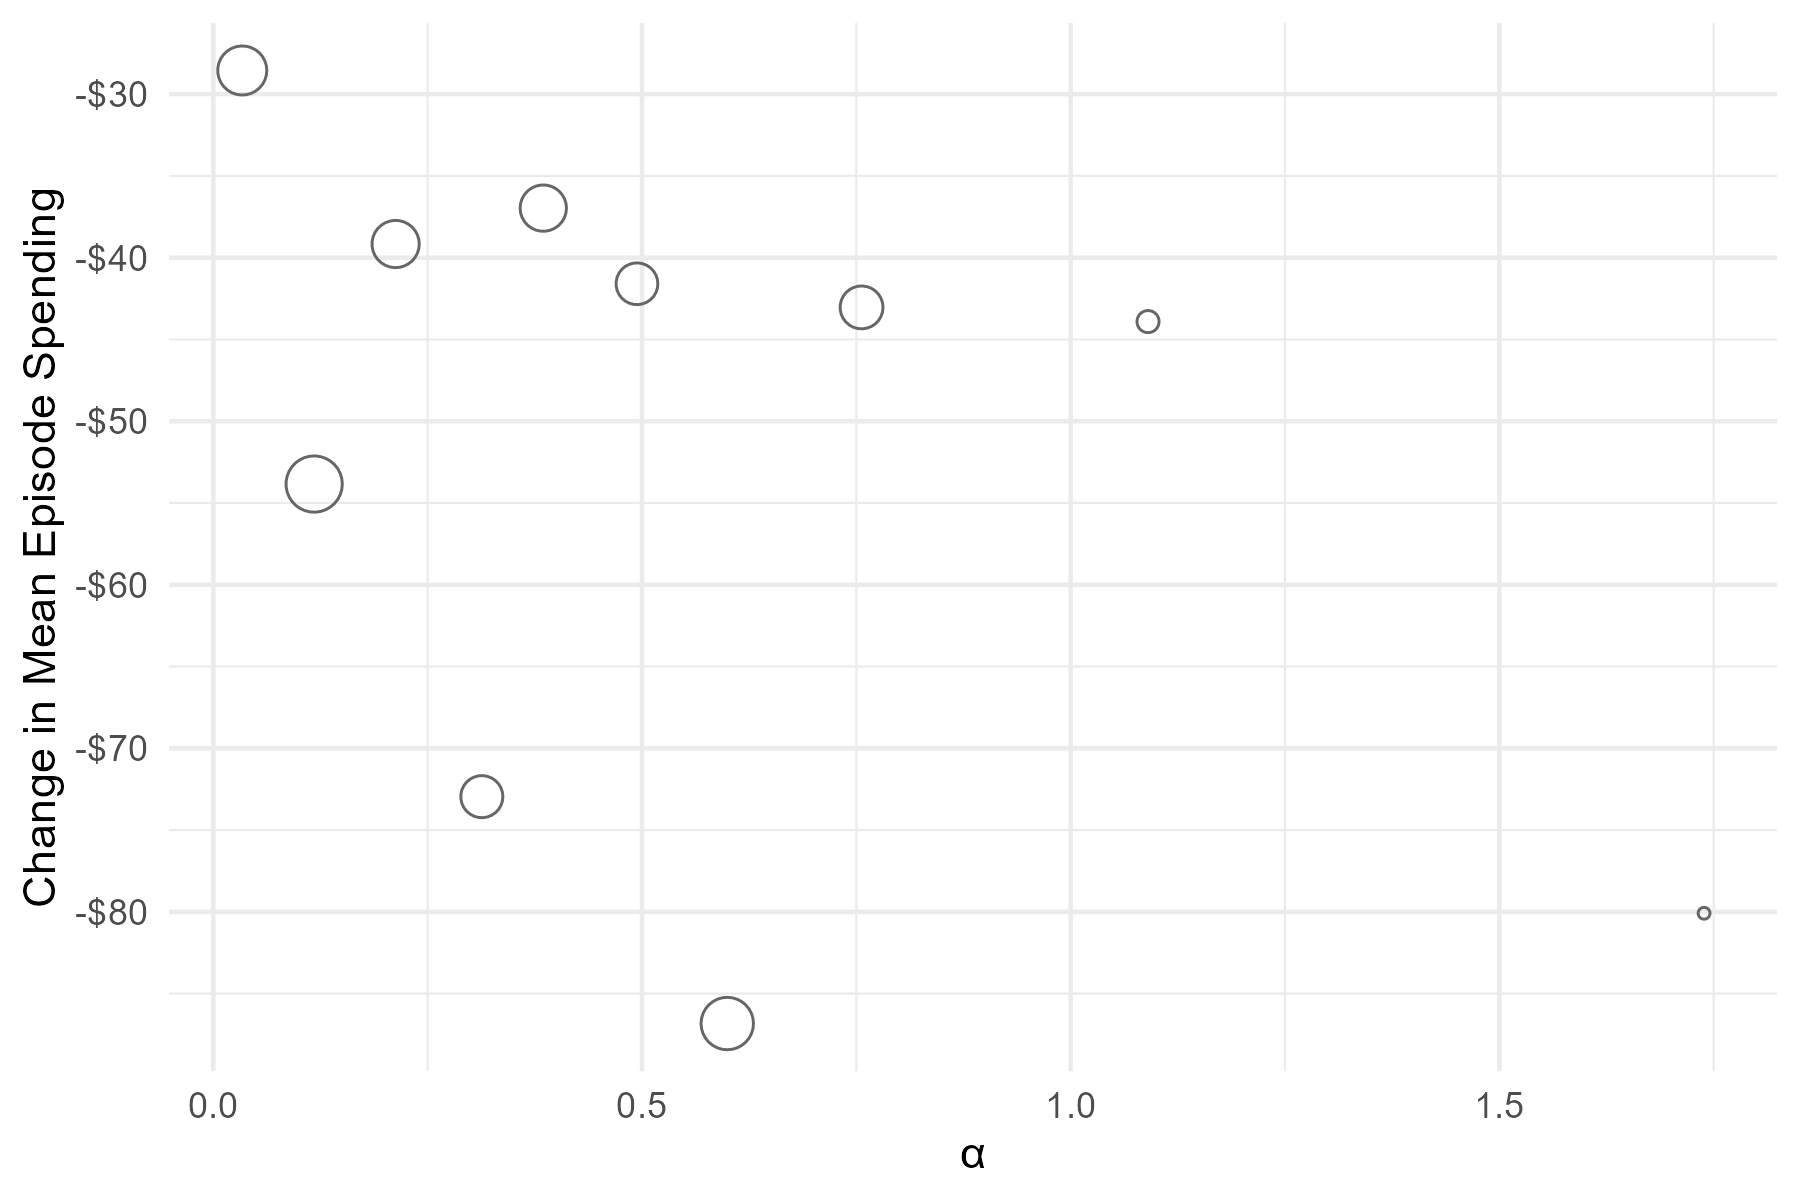
\includegraphics[height=1.6in,width=2.7in,keepaspectratio]{../../../results/figures/myopic-timevary/Gradient_Spend_current_Myopic_eta5.png} & 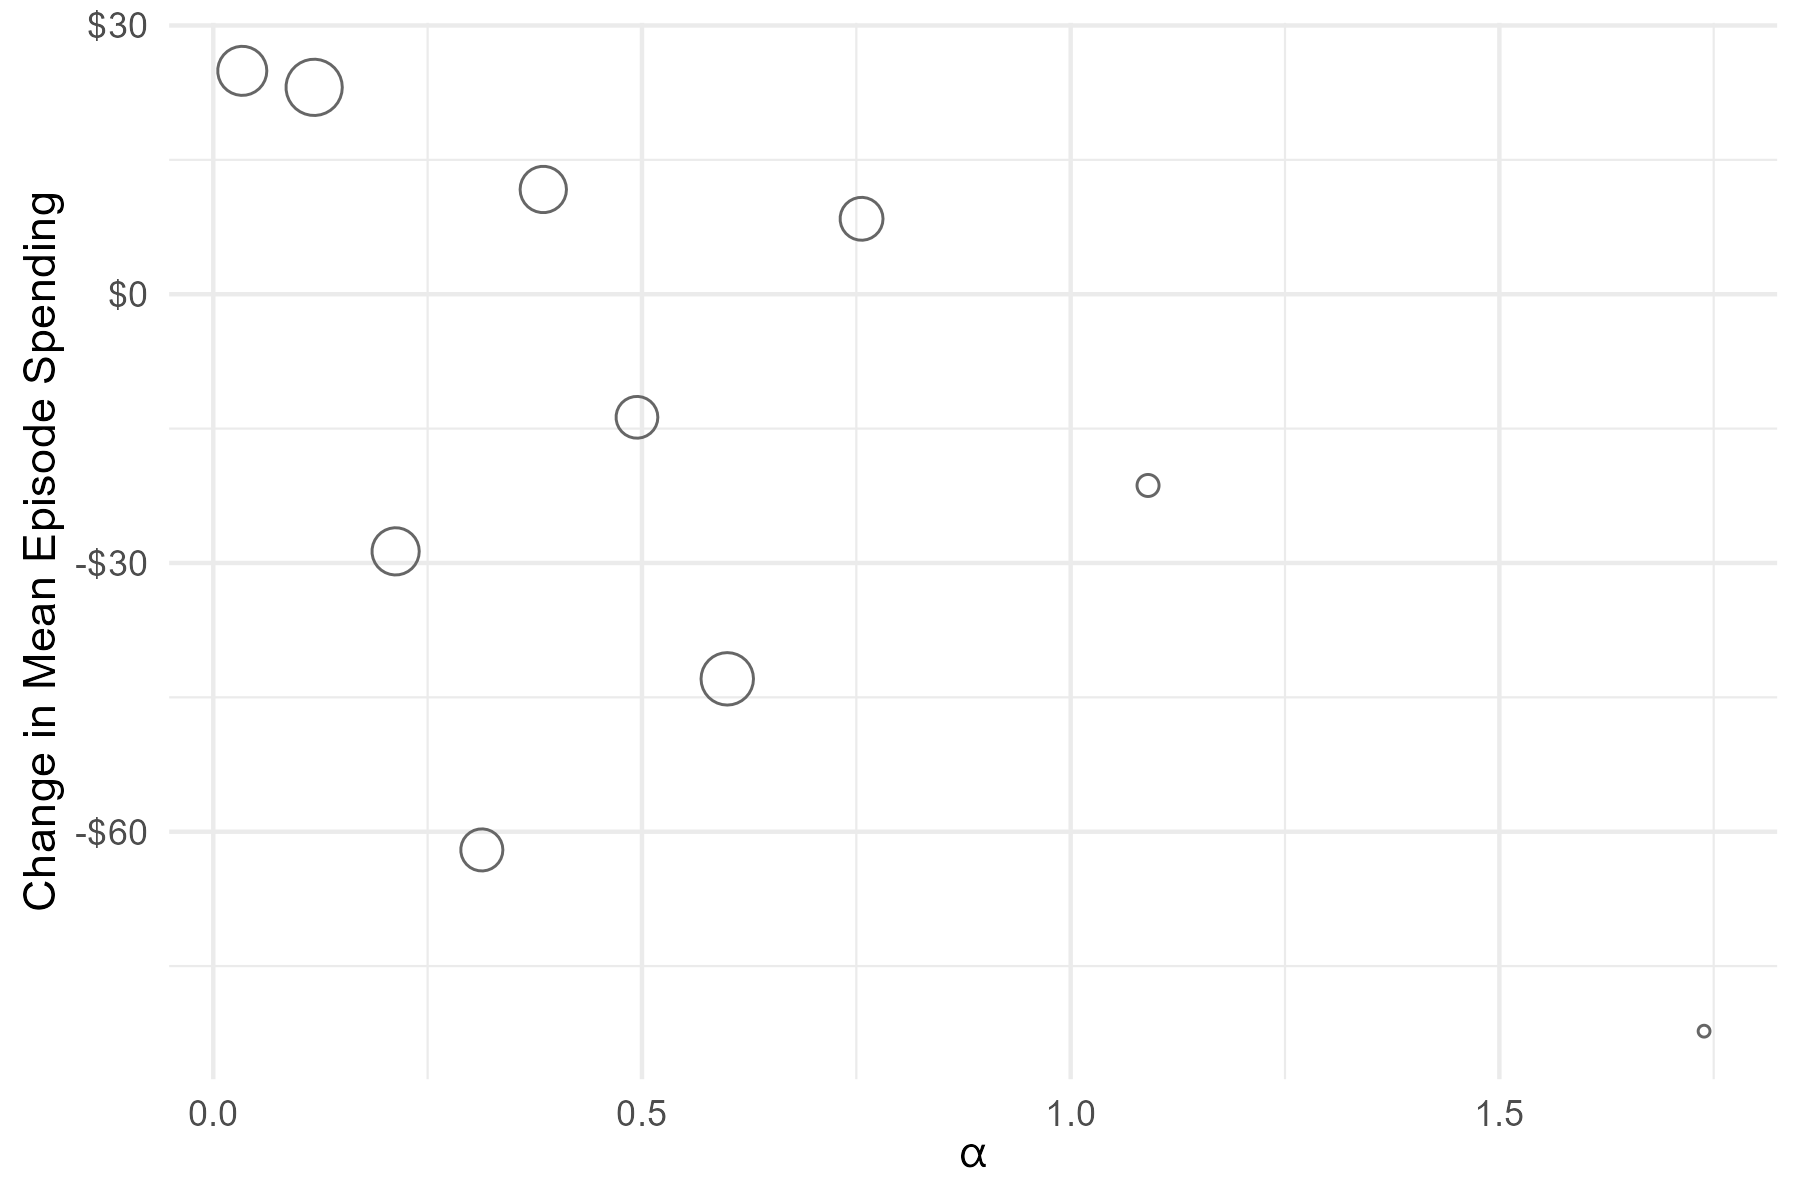
\includegraphics[height=1.6in,width=2.7in,keepaspectratio]{../../../results/figures/myopic-timevary/Gradient_Spend_full_Myopic_eta5.png} \\
\multicolumn{2}{c}{\textit{Forward-looking}} \\
Existing familiarity & Reset familiarity \\
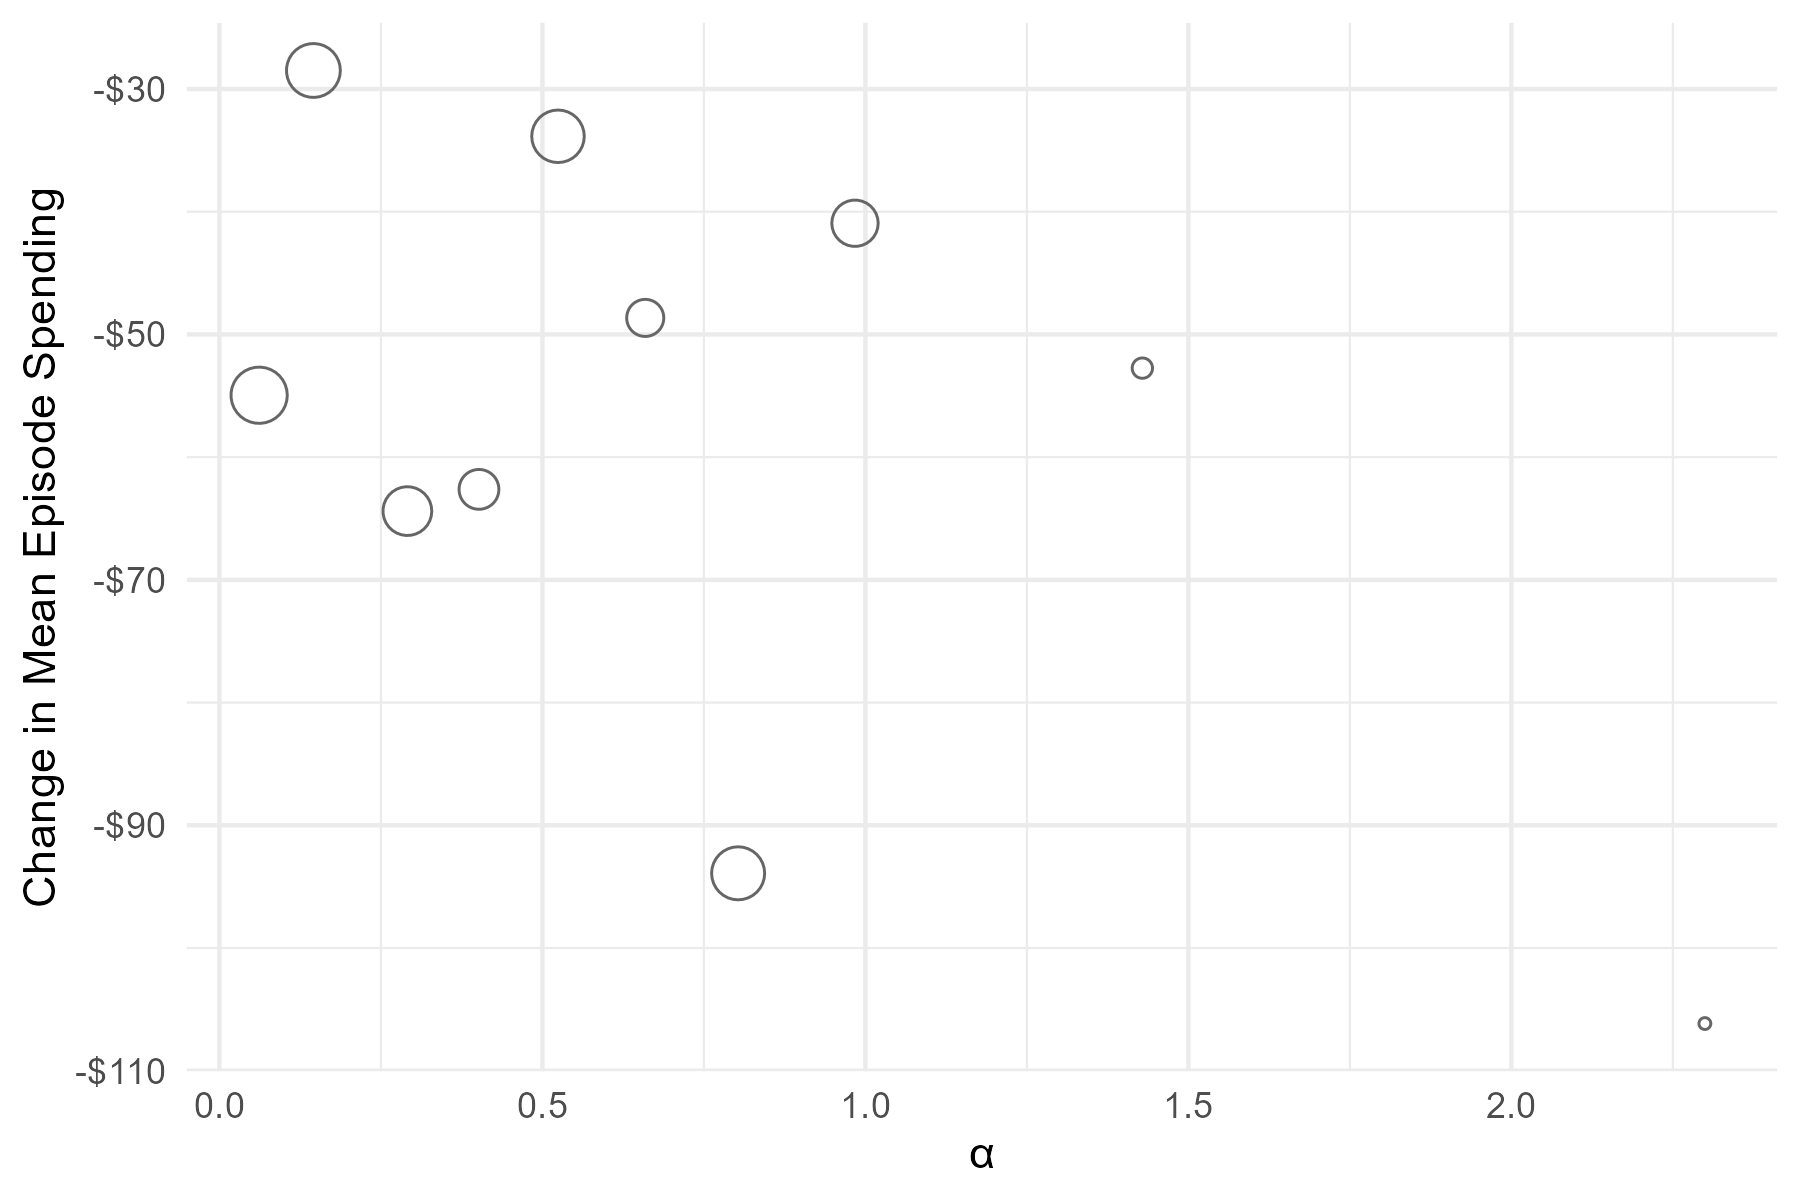
\includegraphics[height=1.6in,width=2.7in,keepaspectratio]{../../../results/figures/fwd-timevary/Gradient_Spend_current_FWD_eta5.png} & 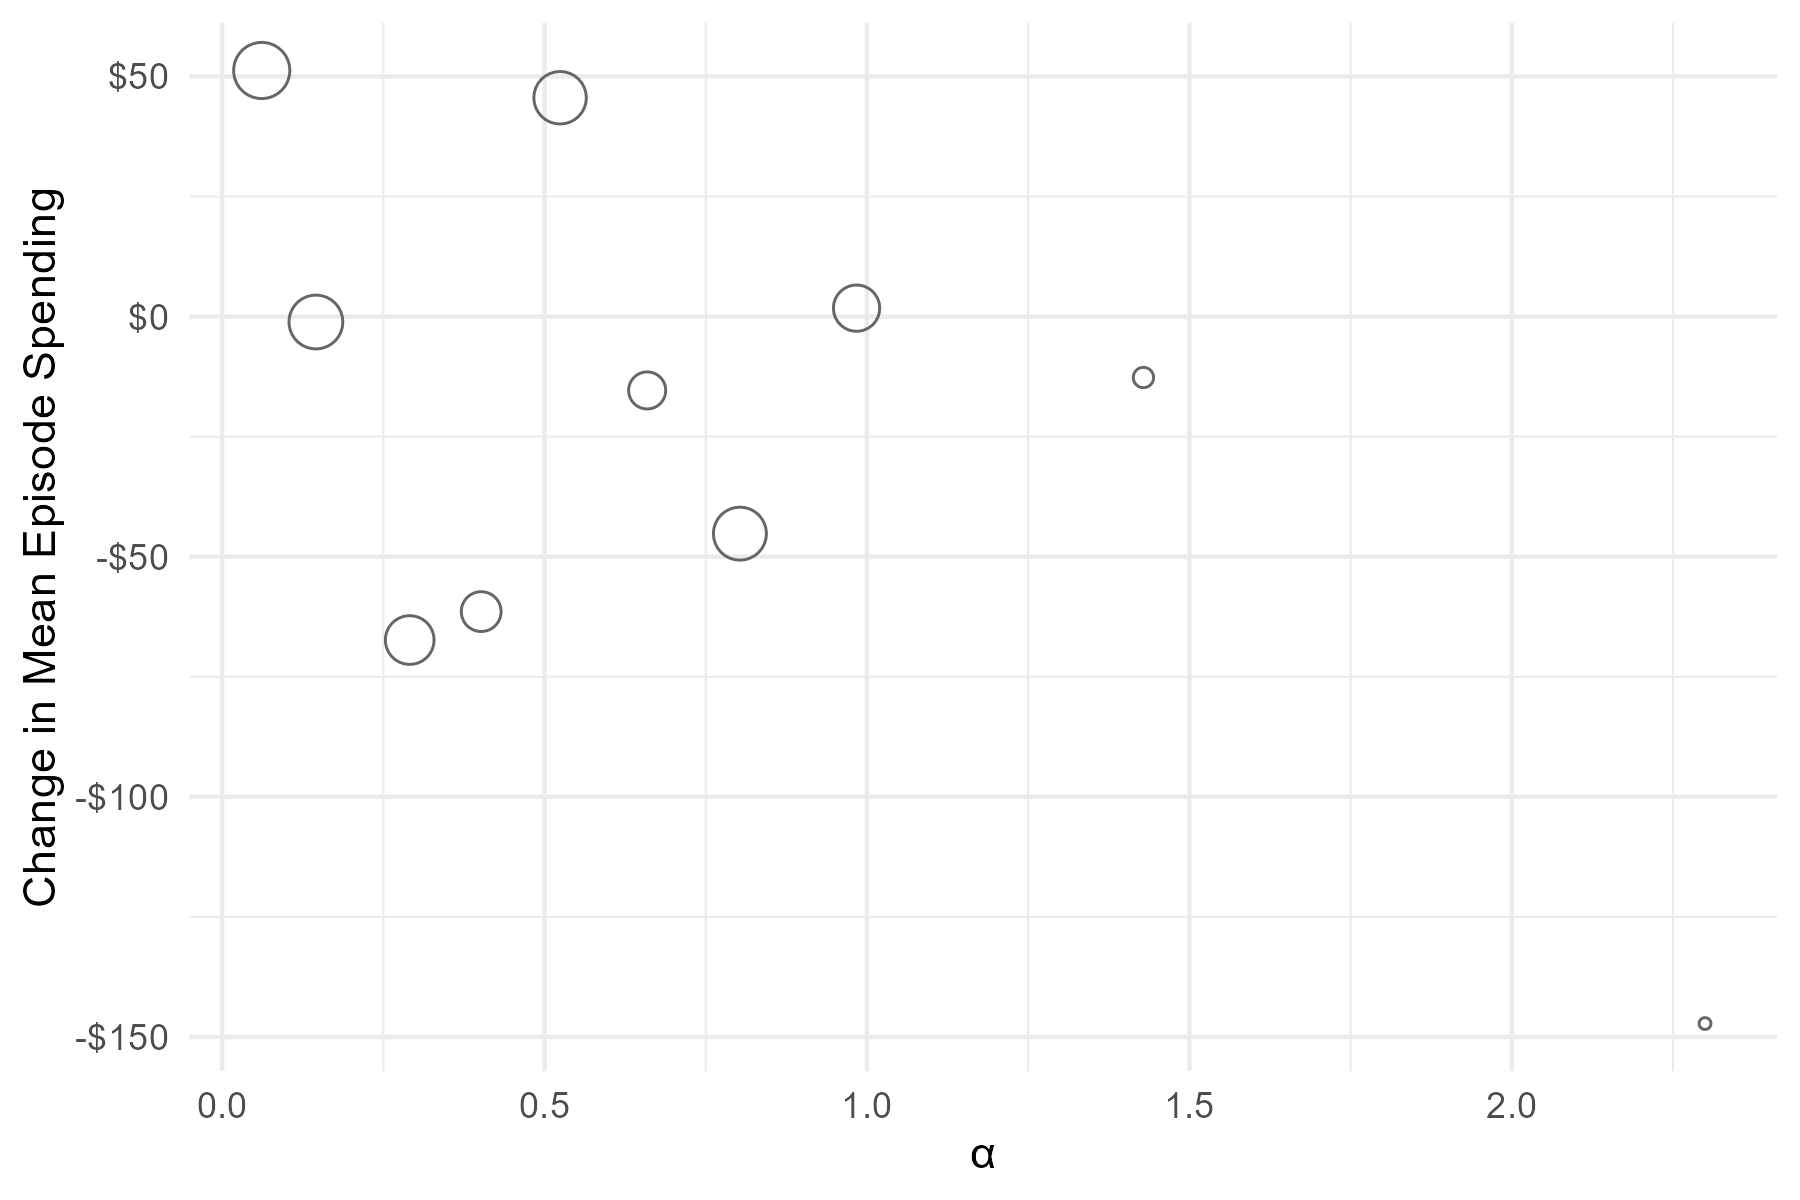
\includegraphics[height=1.6in,width=2.7in,keepaspectratio]{../../../results/figures/fwd-timevary/Gradient_Spend_full_FWD_eta5.png}
\end{tabular}
\label{fig:gradient_spend_eta5}
\end{minipage}
\end{figure}

\clearpage
\begin{figure}[!ht]
\centering
\begin{minipage}[h]{6in}
\caption[QualP10 Off-Diagonal ($\eta=5$)]{Off-Diagonal Scatter of Patient-Weighted 10th-Percentile Quality ($\eta=5$)\footnote{Each point is an HRR where the patient-weighted 10th percentile of specialist quality under the counterfactual differs from the baseline value. HRRs with identical baseline and counterfactual percentile are dropped (they lie on the 45-degree line). The solid reference line is the 45-degree line.}}
\centering
\begin{tabular}{cc}
\multicolumn{2}{c}{\textit{Myopic}} \\
Existing familiarity & Reset familiarity \\
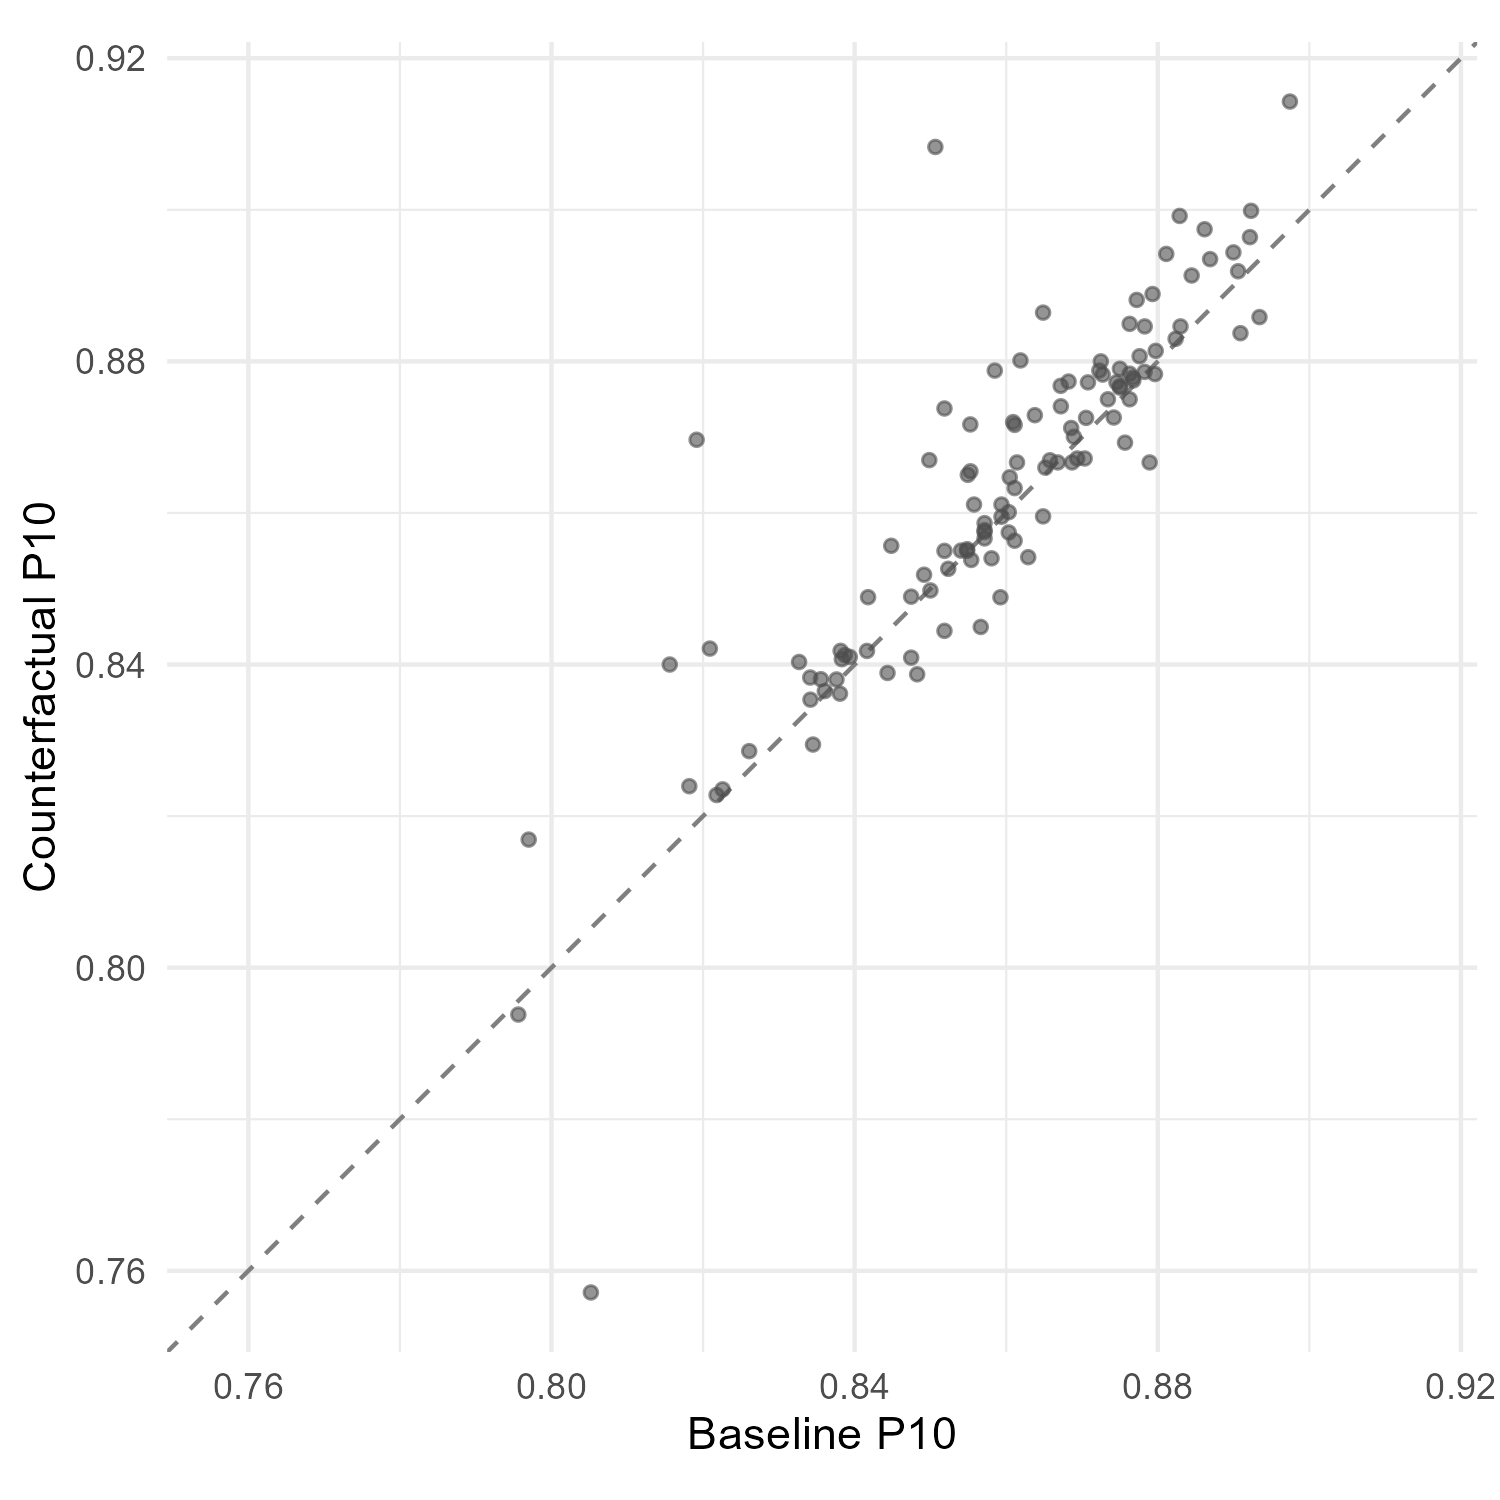
\includegraphics[height=2.2in,width=2.5in,keepaspectratio]{../../../results/figures/myopic-timevary/QualOffDiag_P10_current_Myopic_eta5.png} & 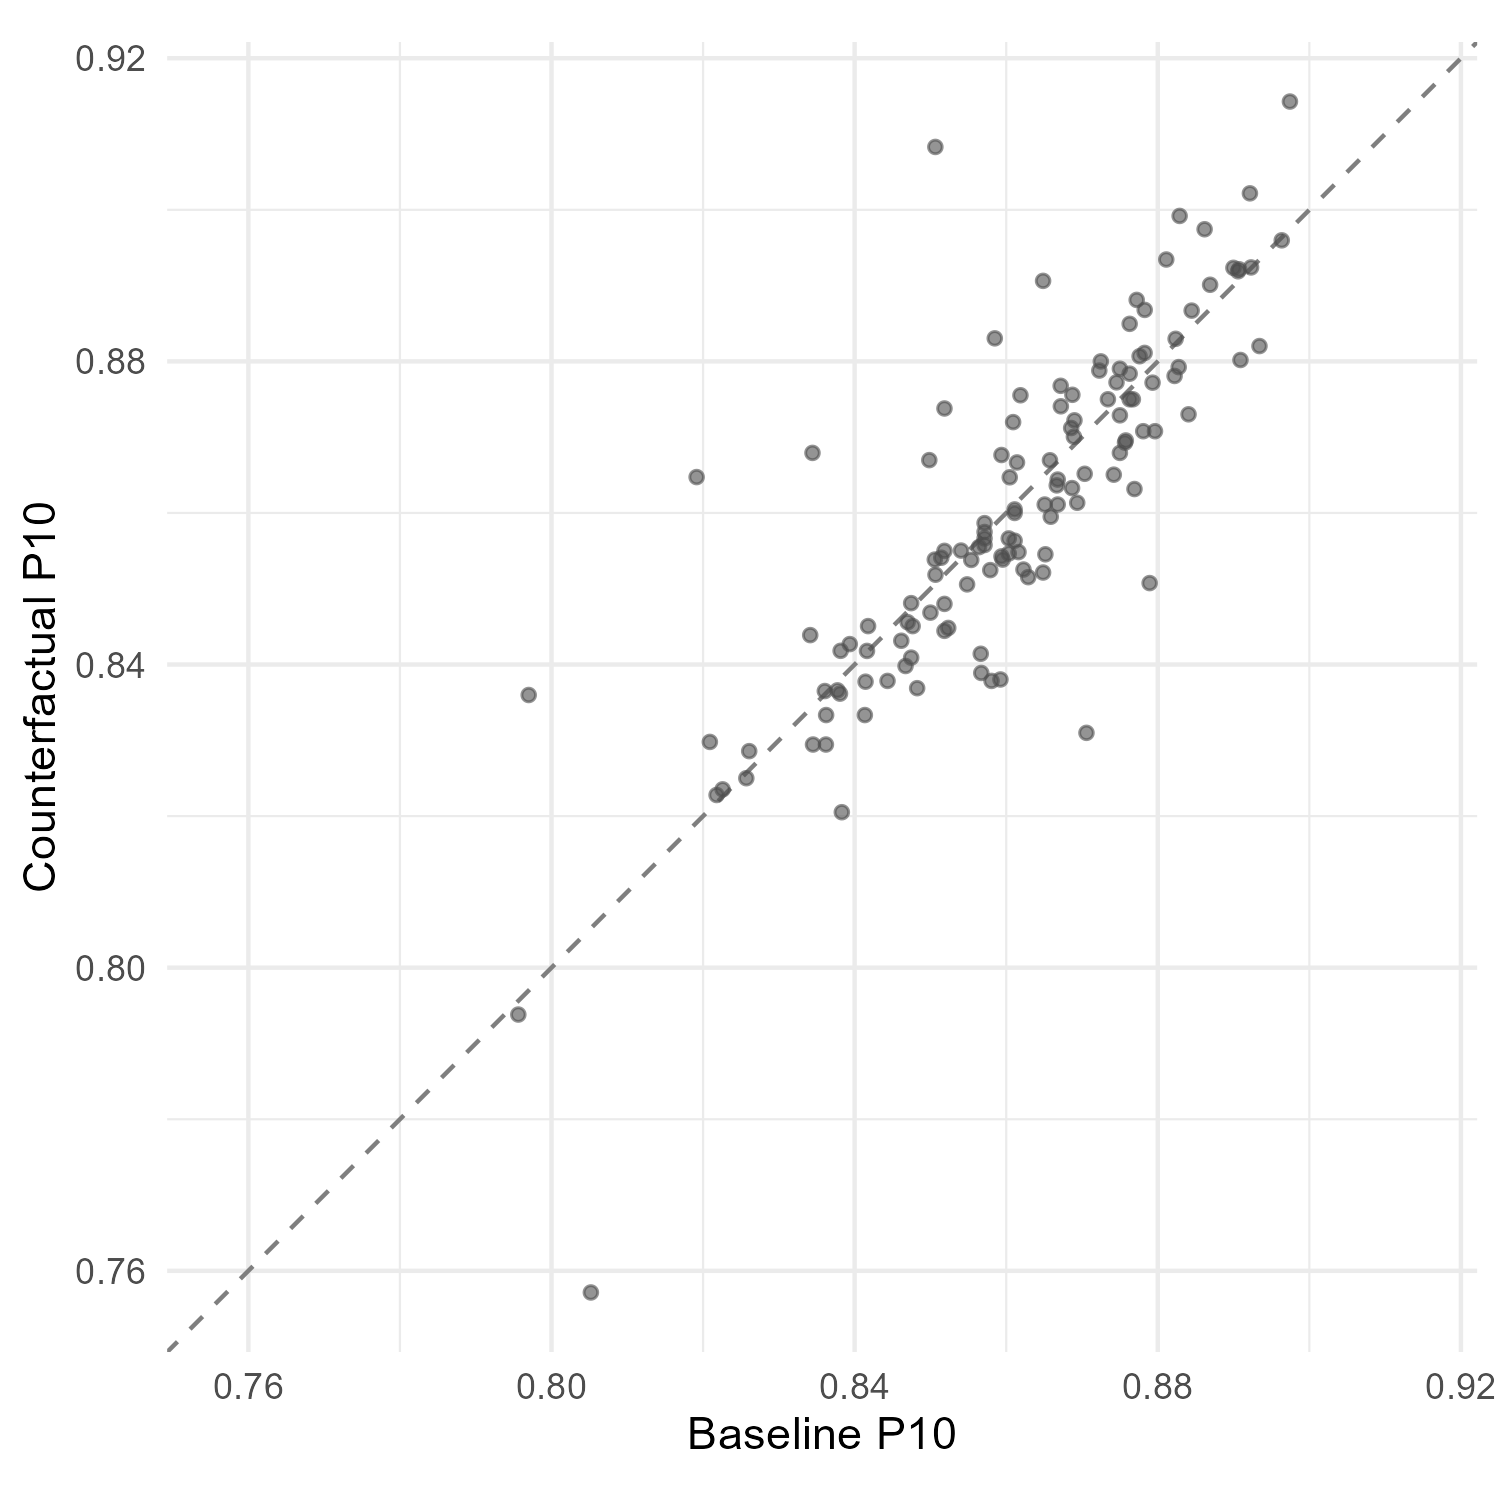
\includegraphics[height=2.2in,width=2.5in,keepaspectratio]{../../../results/figures/myopic-timevary/QualOffDiag_P10_full_Myopic_eta5.png} \\
\multicolumn{2}{c}{\textit{Forward-looking}} \\
Existing familiarity & Reset familiarity \\
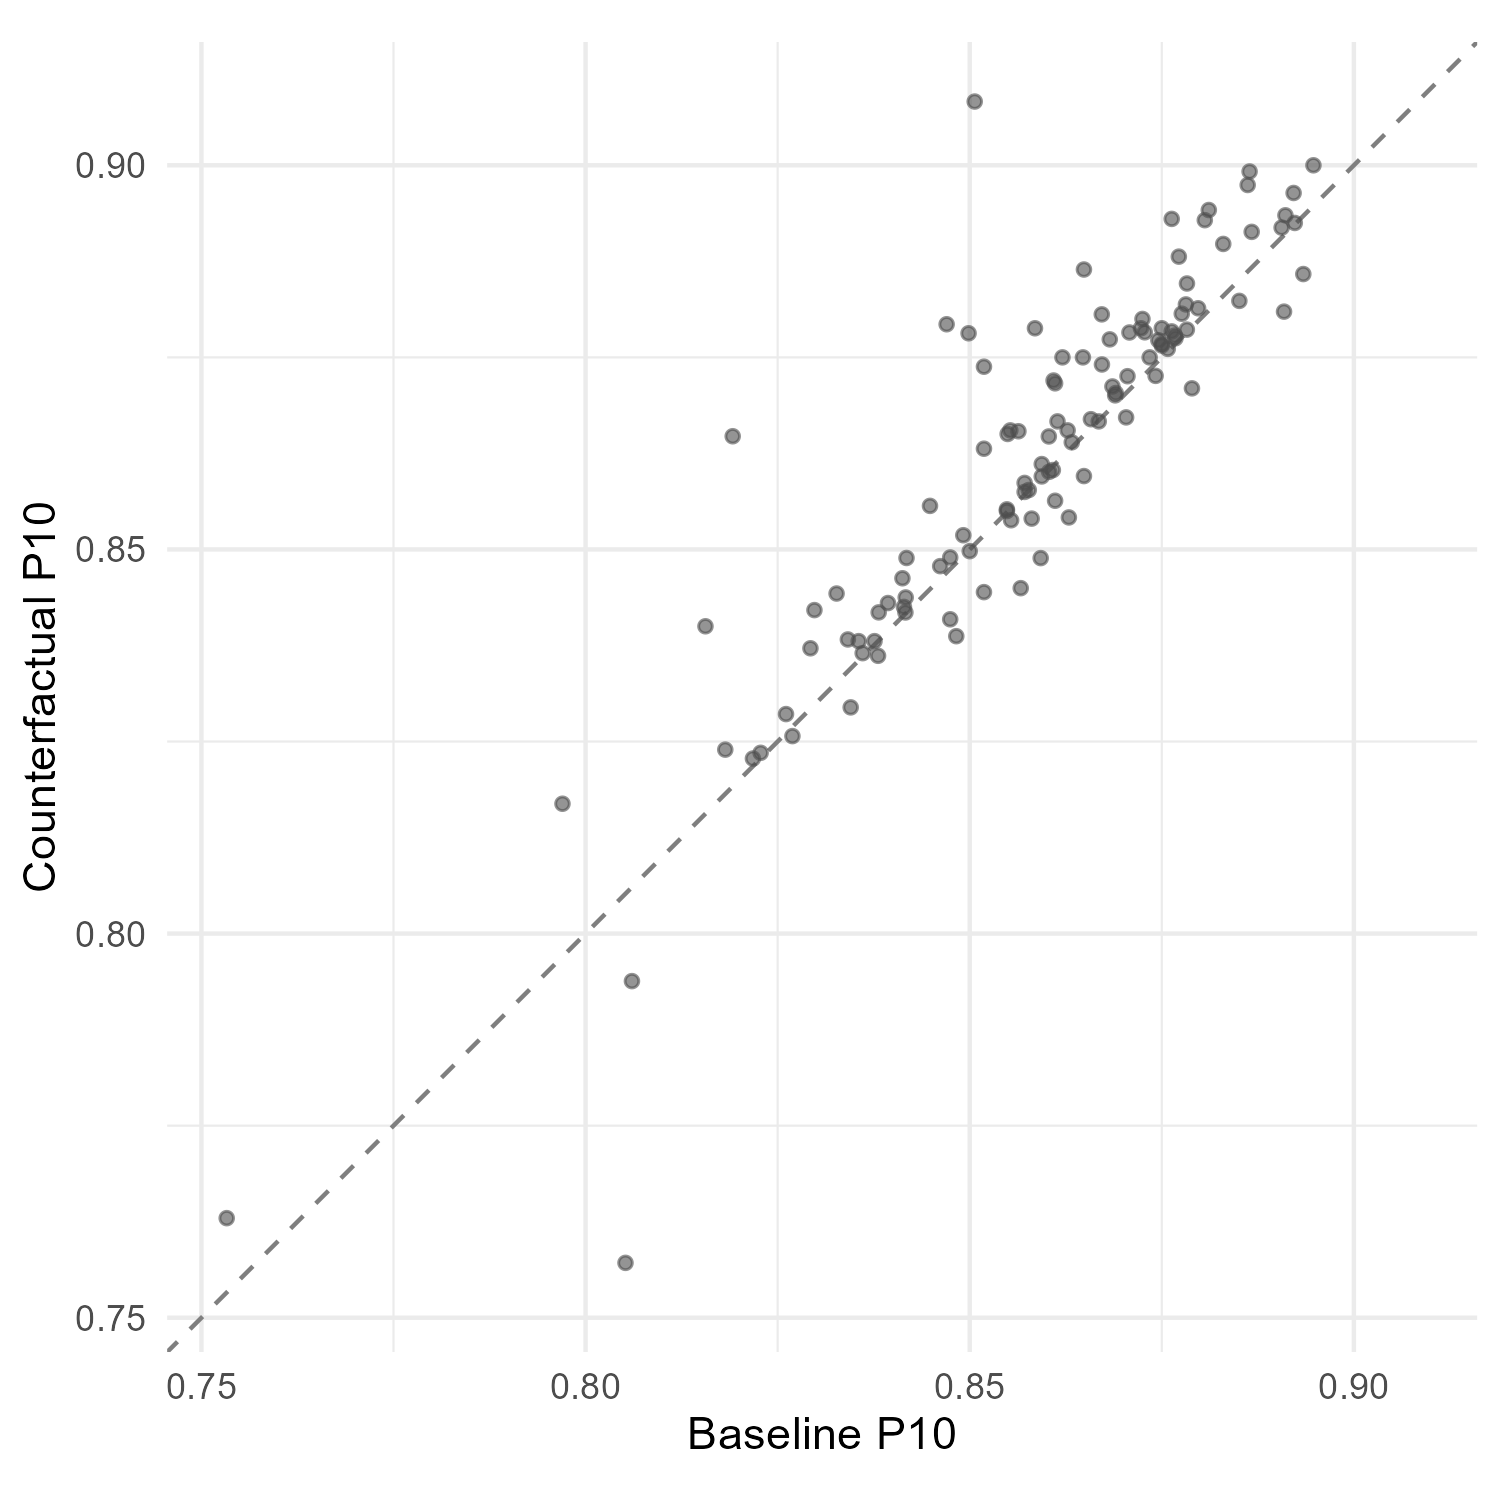
\includegraphics[height=2.2in,width=2.5in,keepaspectratio]{../../../results/figures/fwd-timevary/QualOffDiag_P10_current_FWD_eta5.png} & 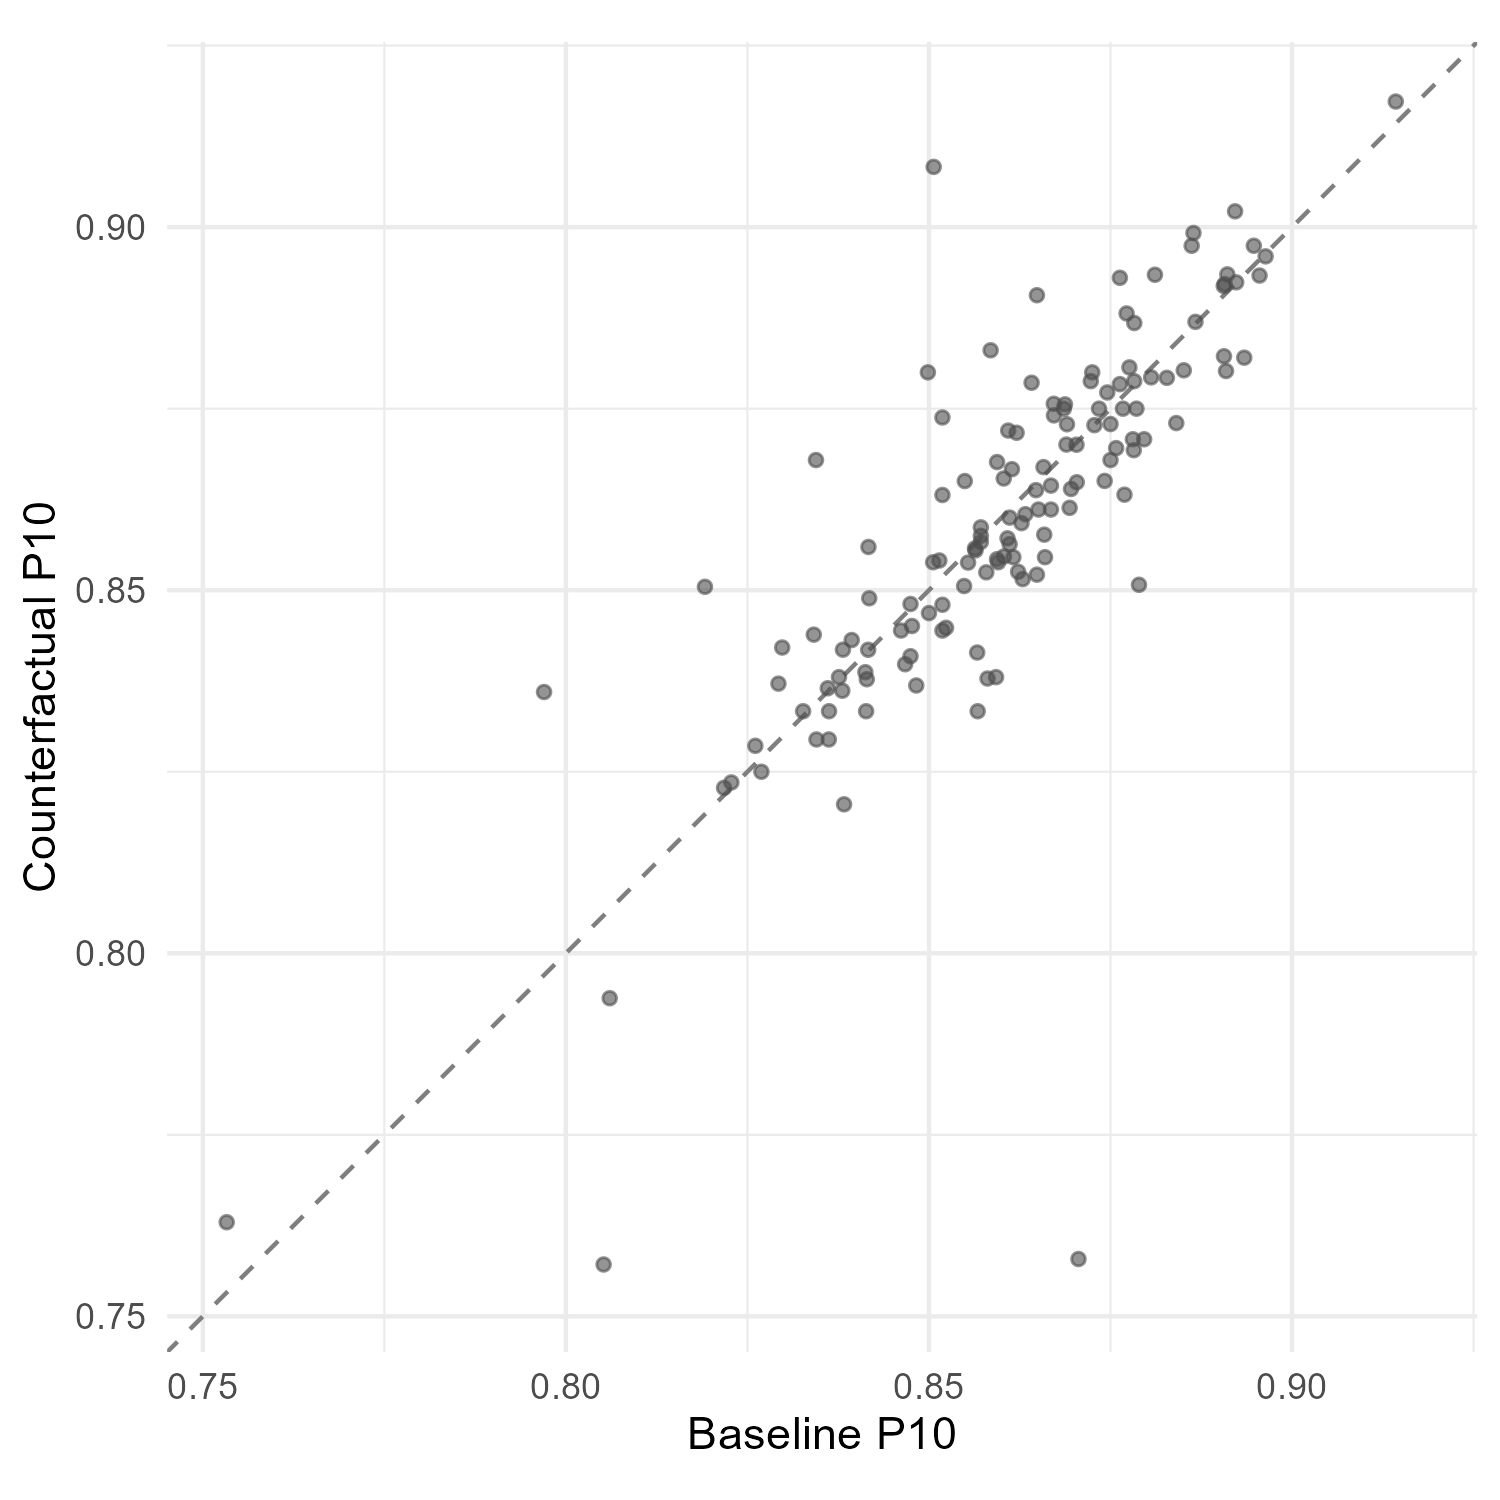
\includegraphics[height=2.2in,width=2.5in,keepaspectratio]{../../../results/figures/fwd-timevary/QualOffDiag_P10_full_FWD_eta5.png}
\end{tabular}
\label{fig:qualP10-cf-eta5}
\end{minipage}
\end{figure}

\clearpage
\begin{figure}[!ht]
\centering
\begin{minipage}[h]{6in}
\caption[QualP90 Off-Diagonal ($\eta=5$)]{Off-Diagonal Scatter of Patient-Weighted 90th-Percentile Quality ($\eta=5$)\footnote{Each point is an HRR where the patient-weighted 90th percentile of specialist quality under the counterfactual differs from the baseline value. HRRs with identical baseline and counterfactual percentile are dropped (they lie on the 45-degree line). The solid reference line is the 45-degree line.}}
\centering
\begin{tabular}{cc}
\multicolumn{2}{c}{\textit{Myopic}} \\
Existing familiarity & Reset familiarity \\
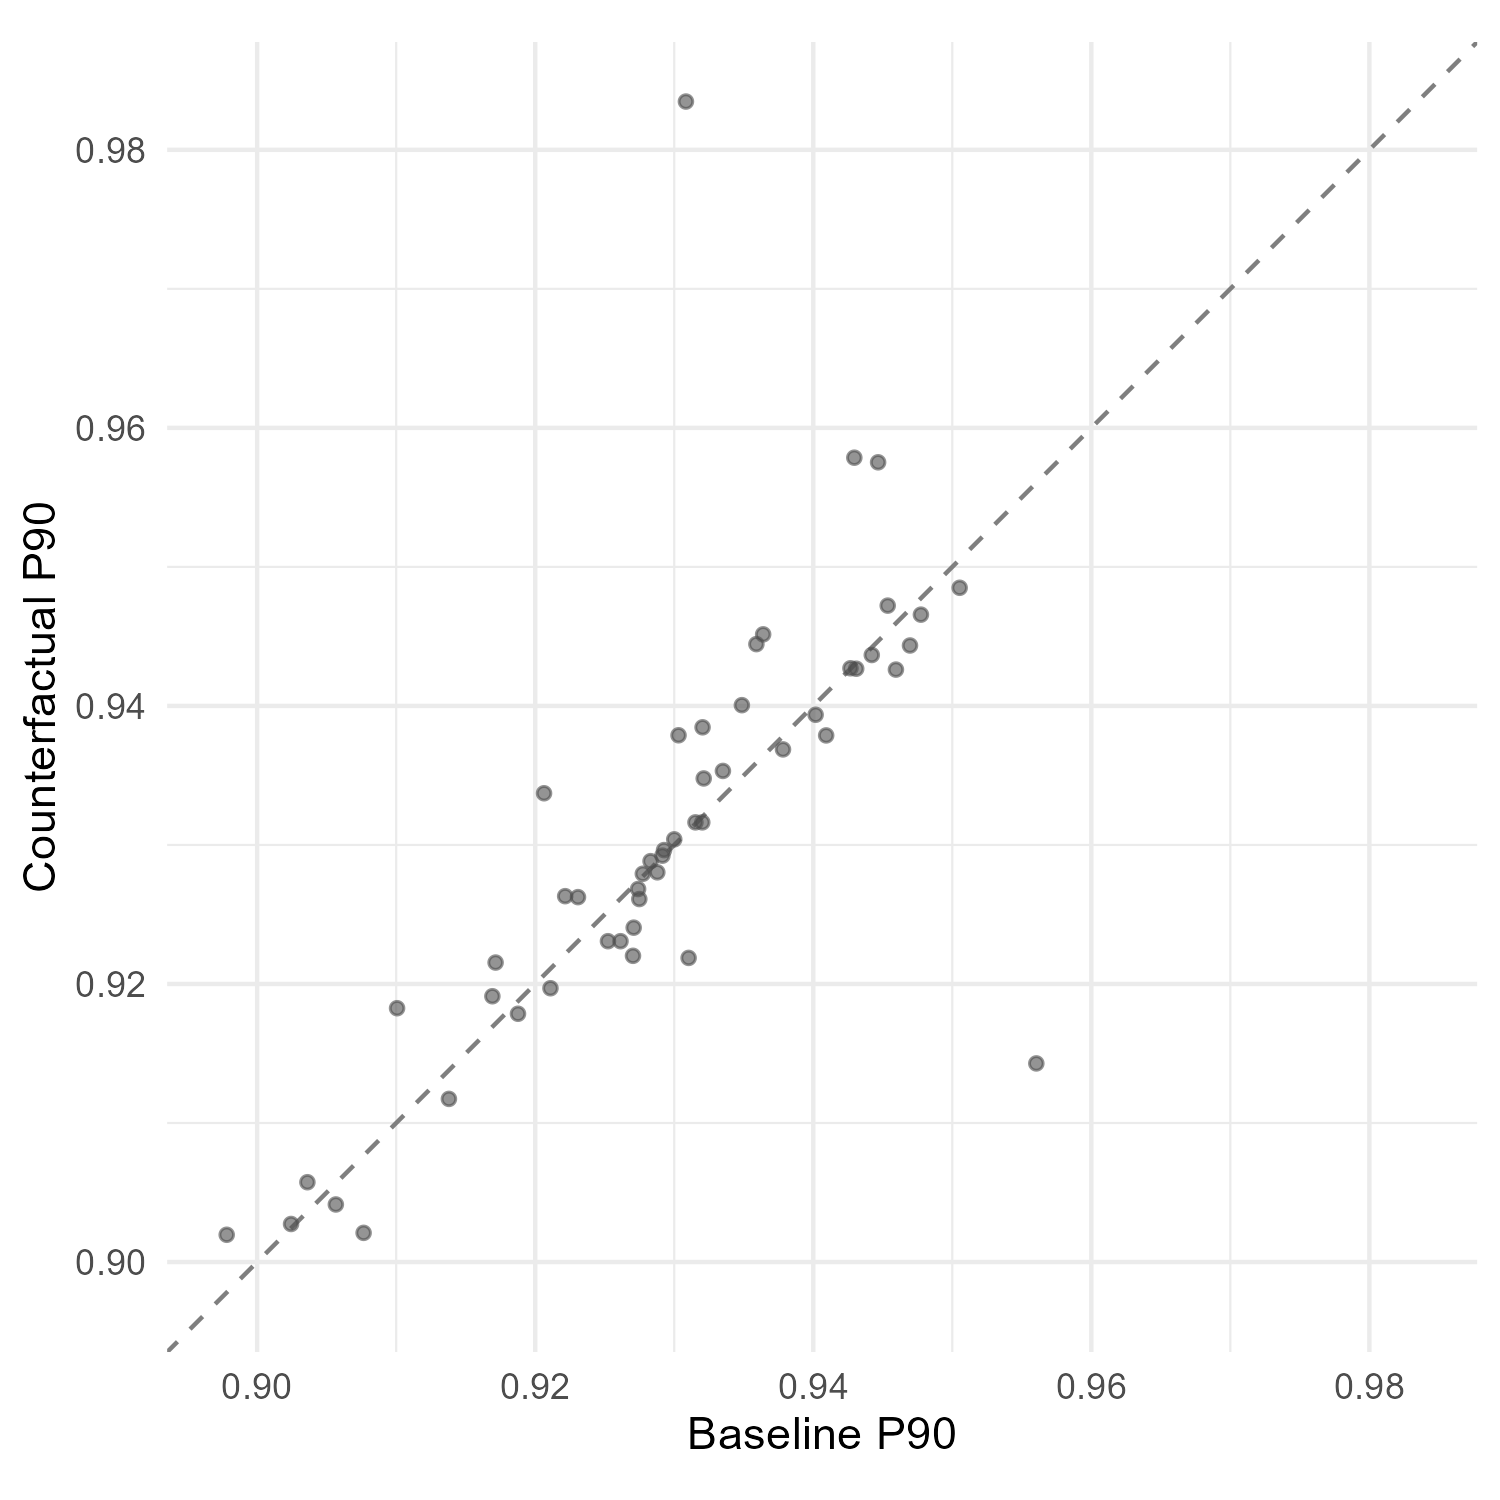
\includegraphics[height=2.2in,width=2.5in,keepaspectratio]{../../../results/figures/myopic-timevary/QualOffDiag_P90_current_Myopic_eta5.png} & 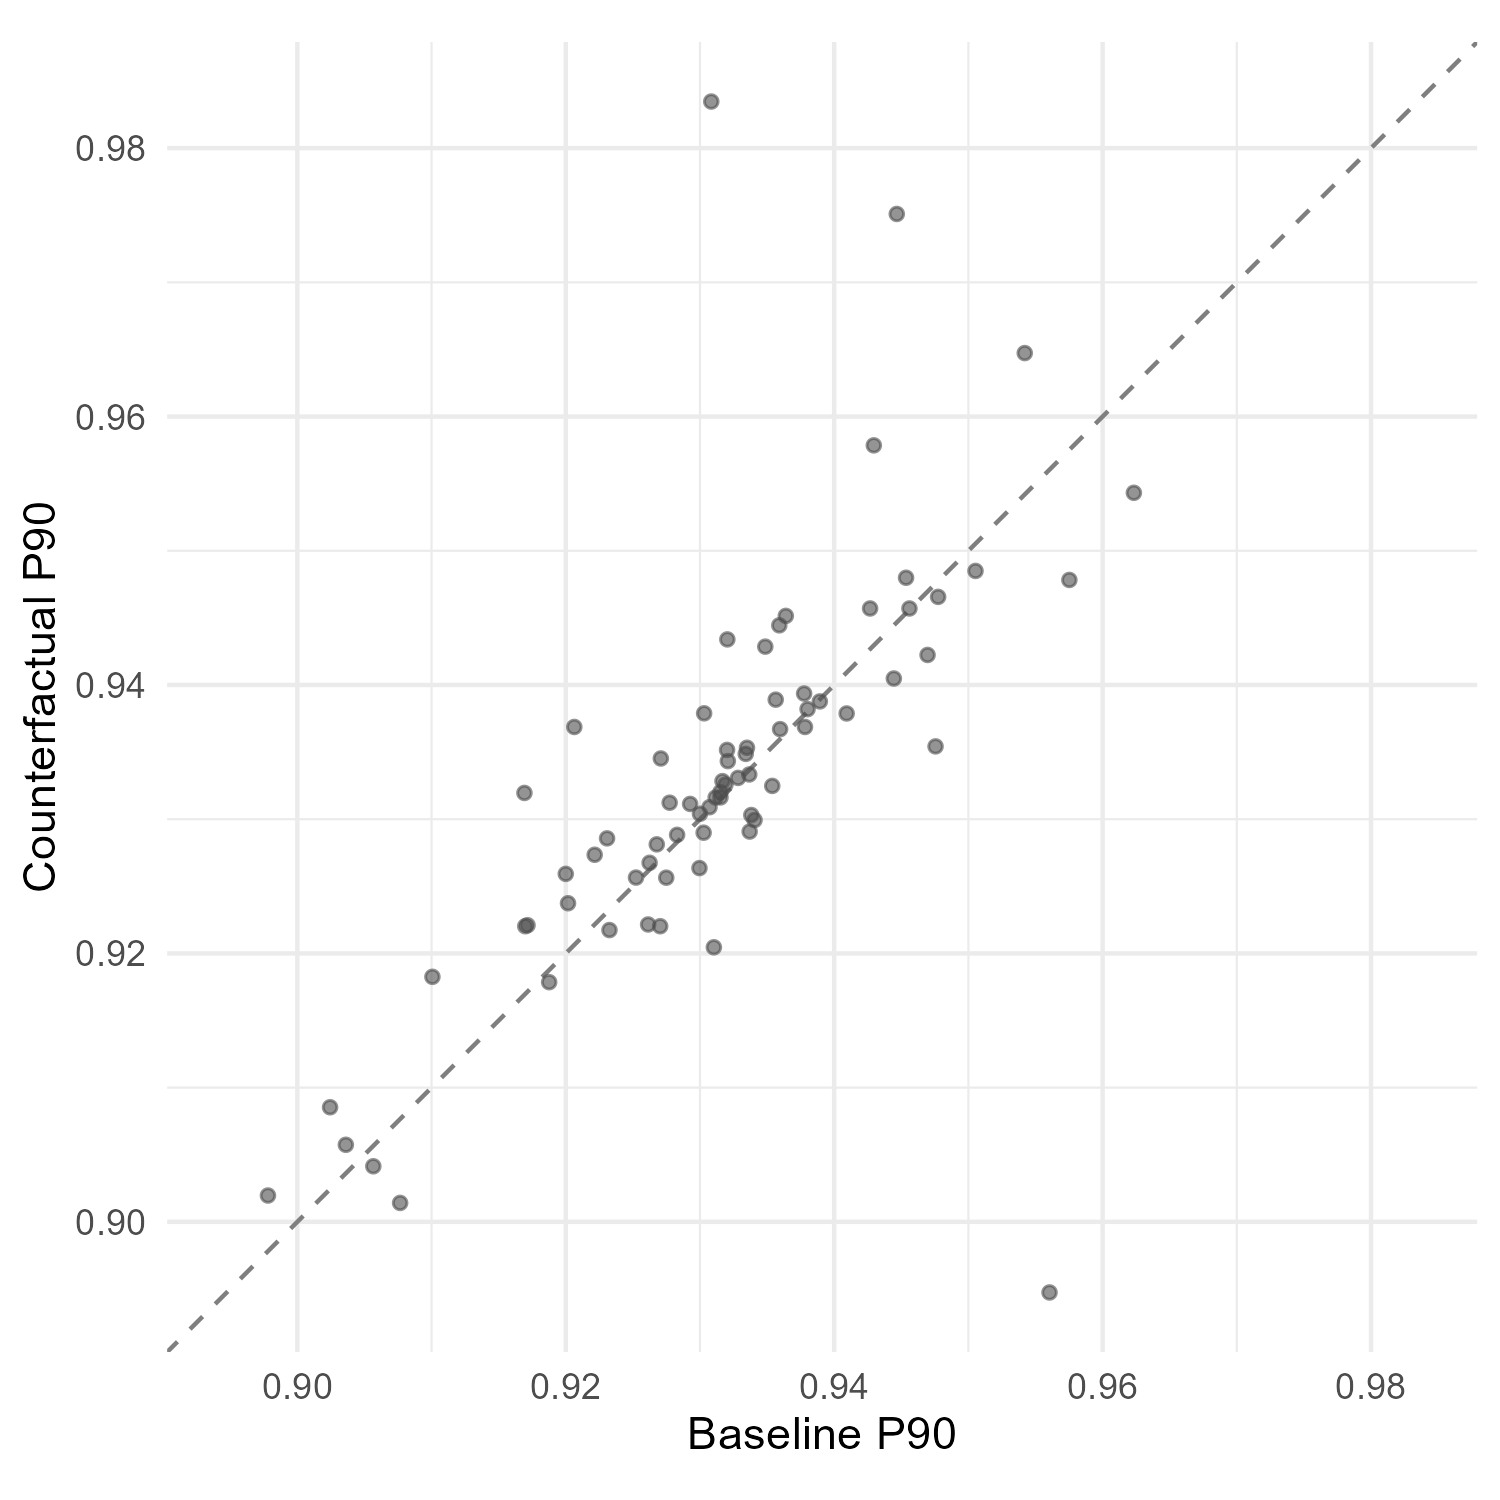
\includegraphics[height=2.2in,width=2.5in,keepaspectratio]{../../../results/figures/myopic-timevary/QualOffDiag_P90_full_Myopic_eta5.png} \\
\multicolumn{2}{c}{\textit{Forward-looking}} \\
Existing familiarity & Reset familiarity \\
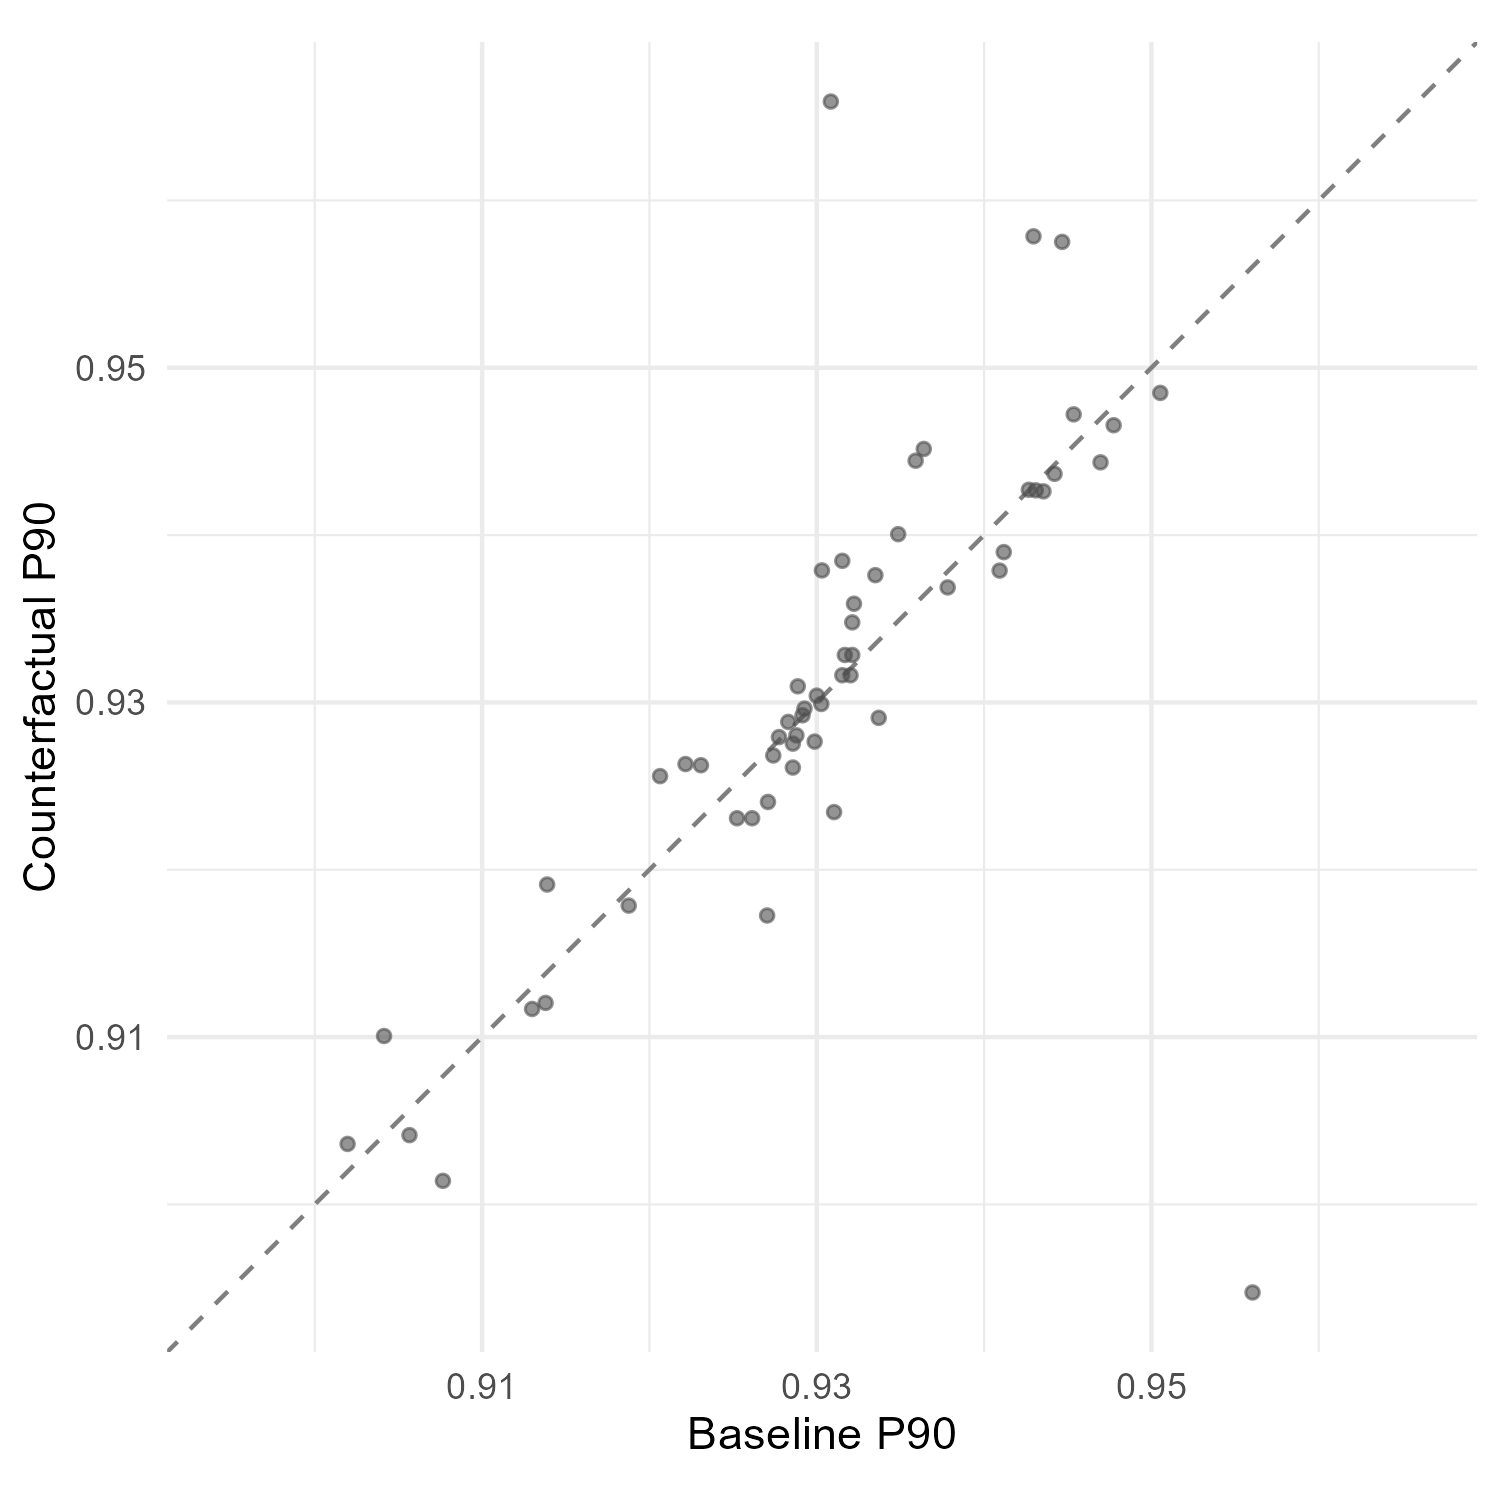
\includegraphics[height=2.2in,width=2.5in,keepaspectratio]{../../../results/figures/fwd-timevary/QualOffDiag_P90_current_FWD_eta5.png} & 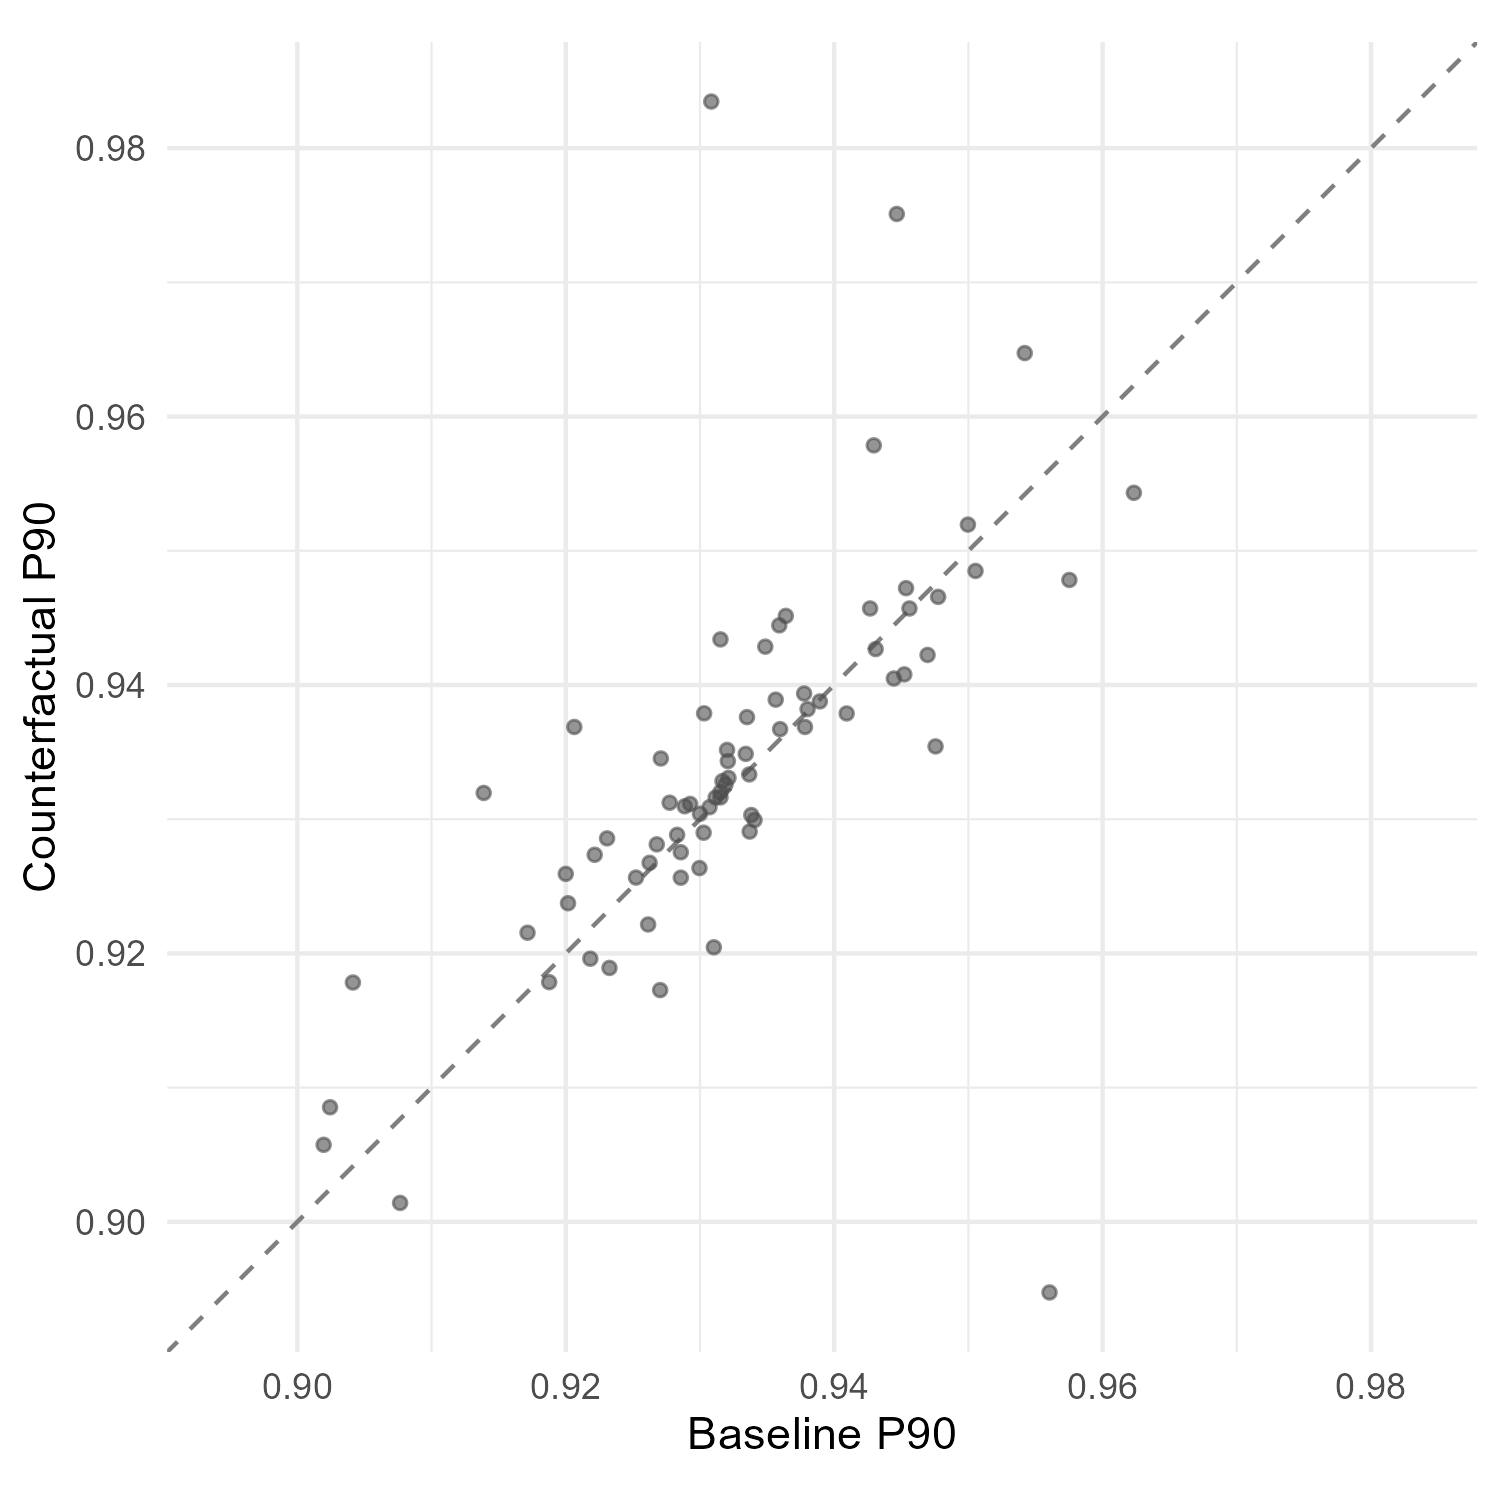
\includegraphics[height=2.2in,width=2.5in,keepaspectratio]{../../../results/figures/fwd-timevary/QualOffDiag_P90_full_FWD_eta5.png}
\end{tabular}
\label{fig:qualP90-cf-eta5}
\end{minipage}
\end{figure}

\clearpage
\begin{figure}[!ht]
\centering
\begin{minipage}[h]{6in}
\caption[SpendP10 Off-Diagonal ($\eta=5$)]{Off-Diagonal Scatter of Patient-Weighted 10th-Percentile Spending ($\eta=5$)\footnote{Each point is an HRR where the patient-weighted 10th percentile of episode spending under the counterfactual differs from the baseline value. HRRs with identical baseline and counterfactual percentile are dropped (they lie on the 45-degree line). The solid reference line is the 45-degree line.}}
\centering
\begin{tabular}{cc}
\multicolumn{2}{c}{\textit{Myopic}} \\
Existing familiarity & Reset familiarity \\
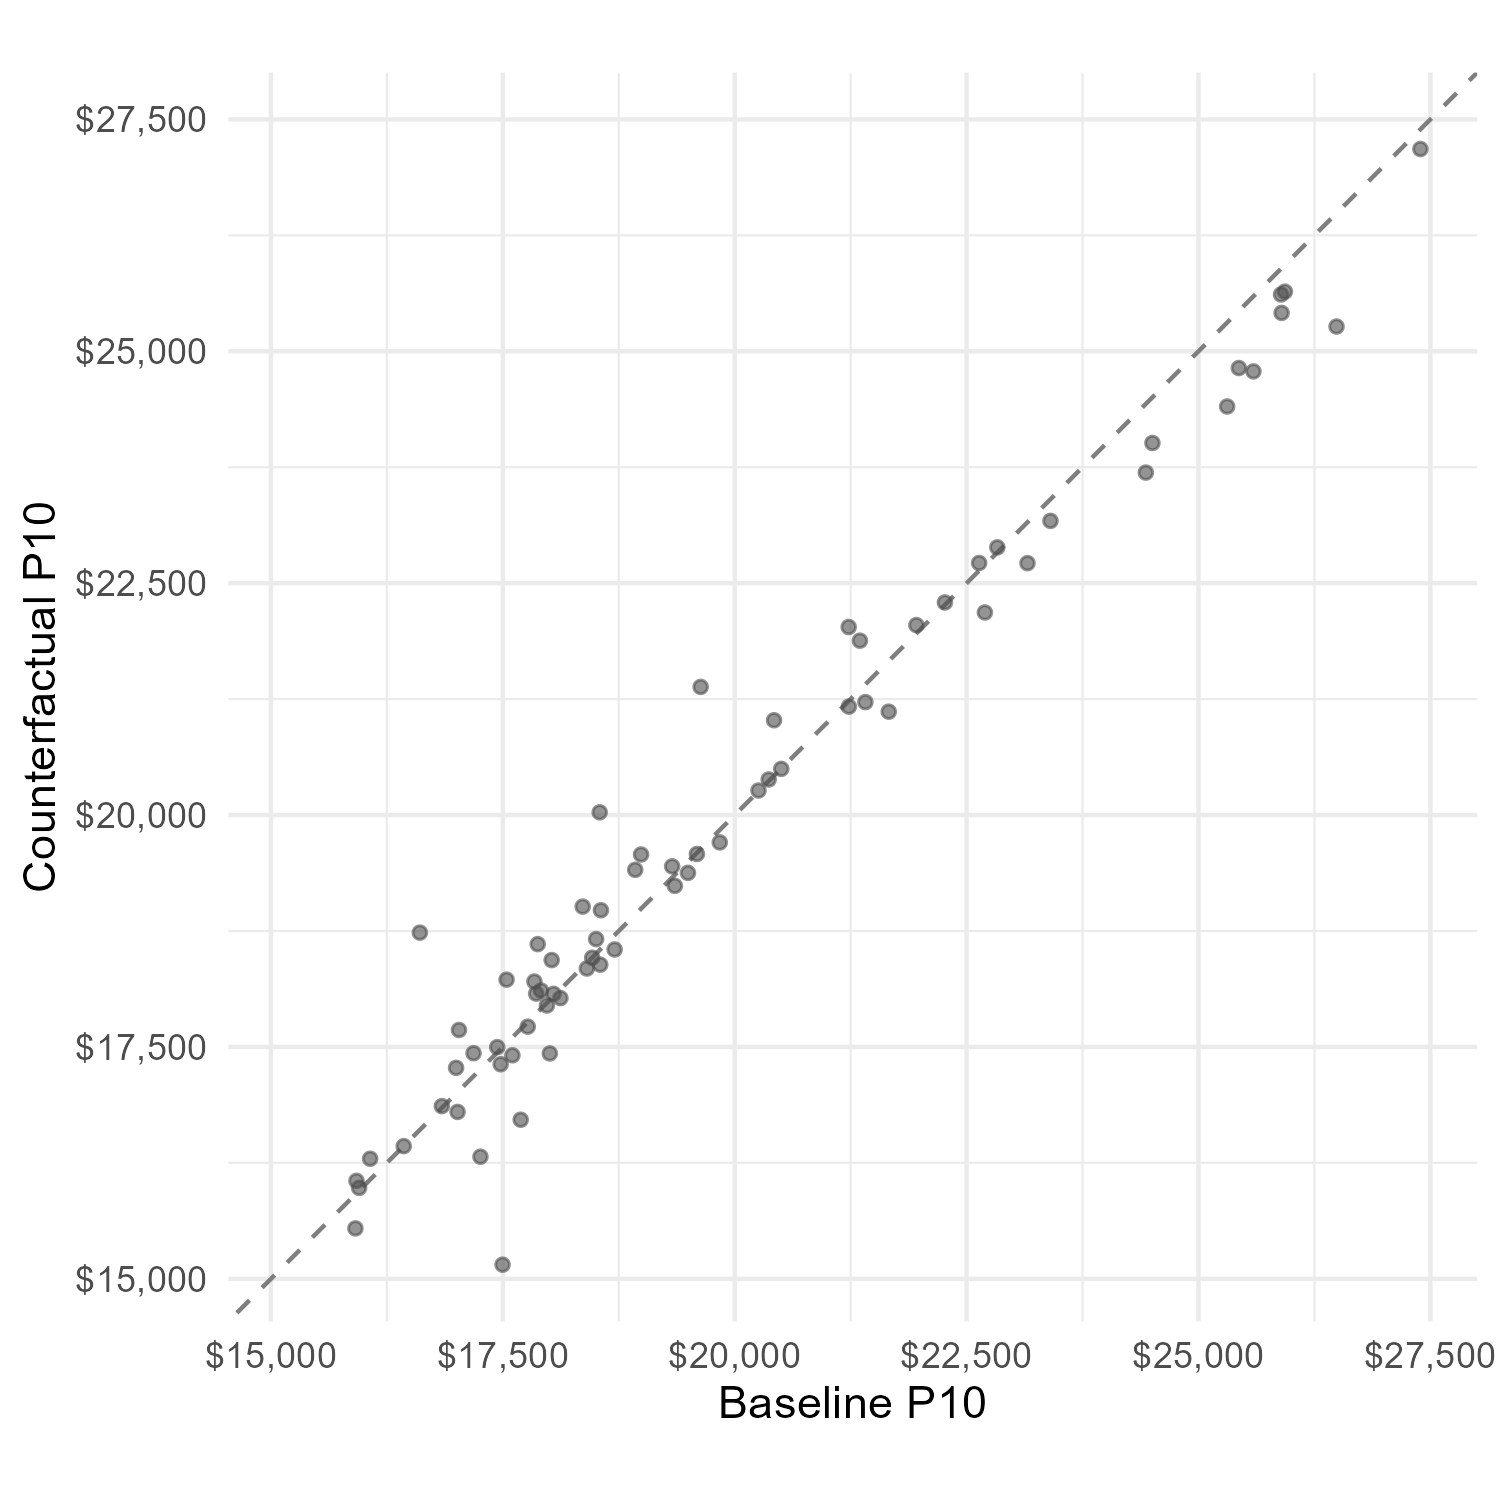
\includegraphics[height=2.2in,width=2.5in,keepaspectratio]{../../../results/figures/myopic-timevary/SpendOffDiag_P10_current_Myopic_eta5.png} & 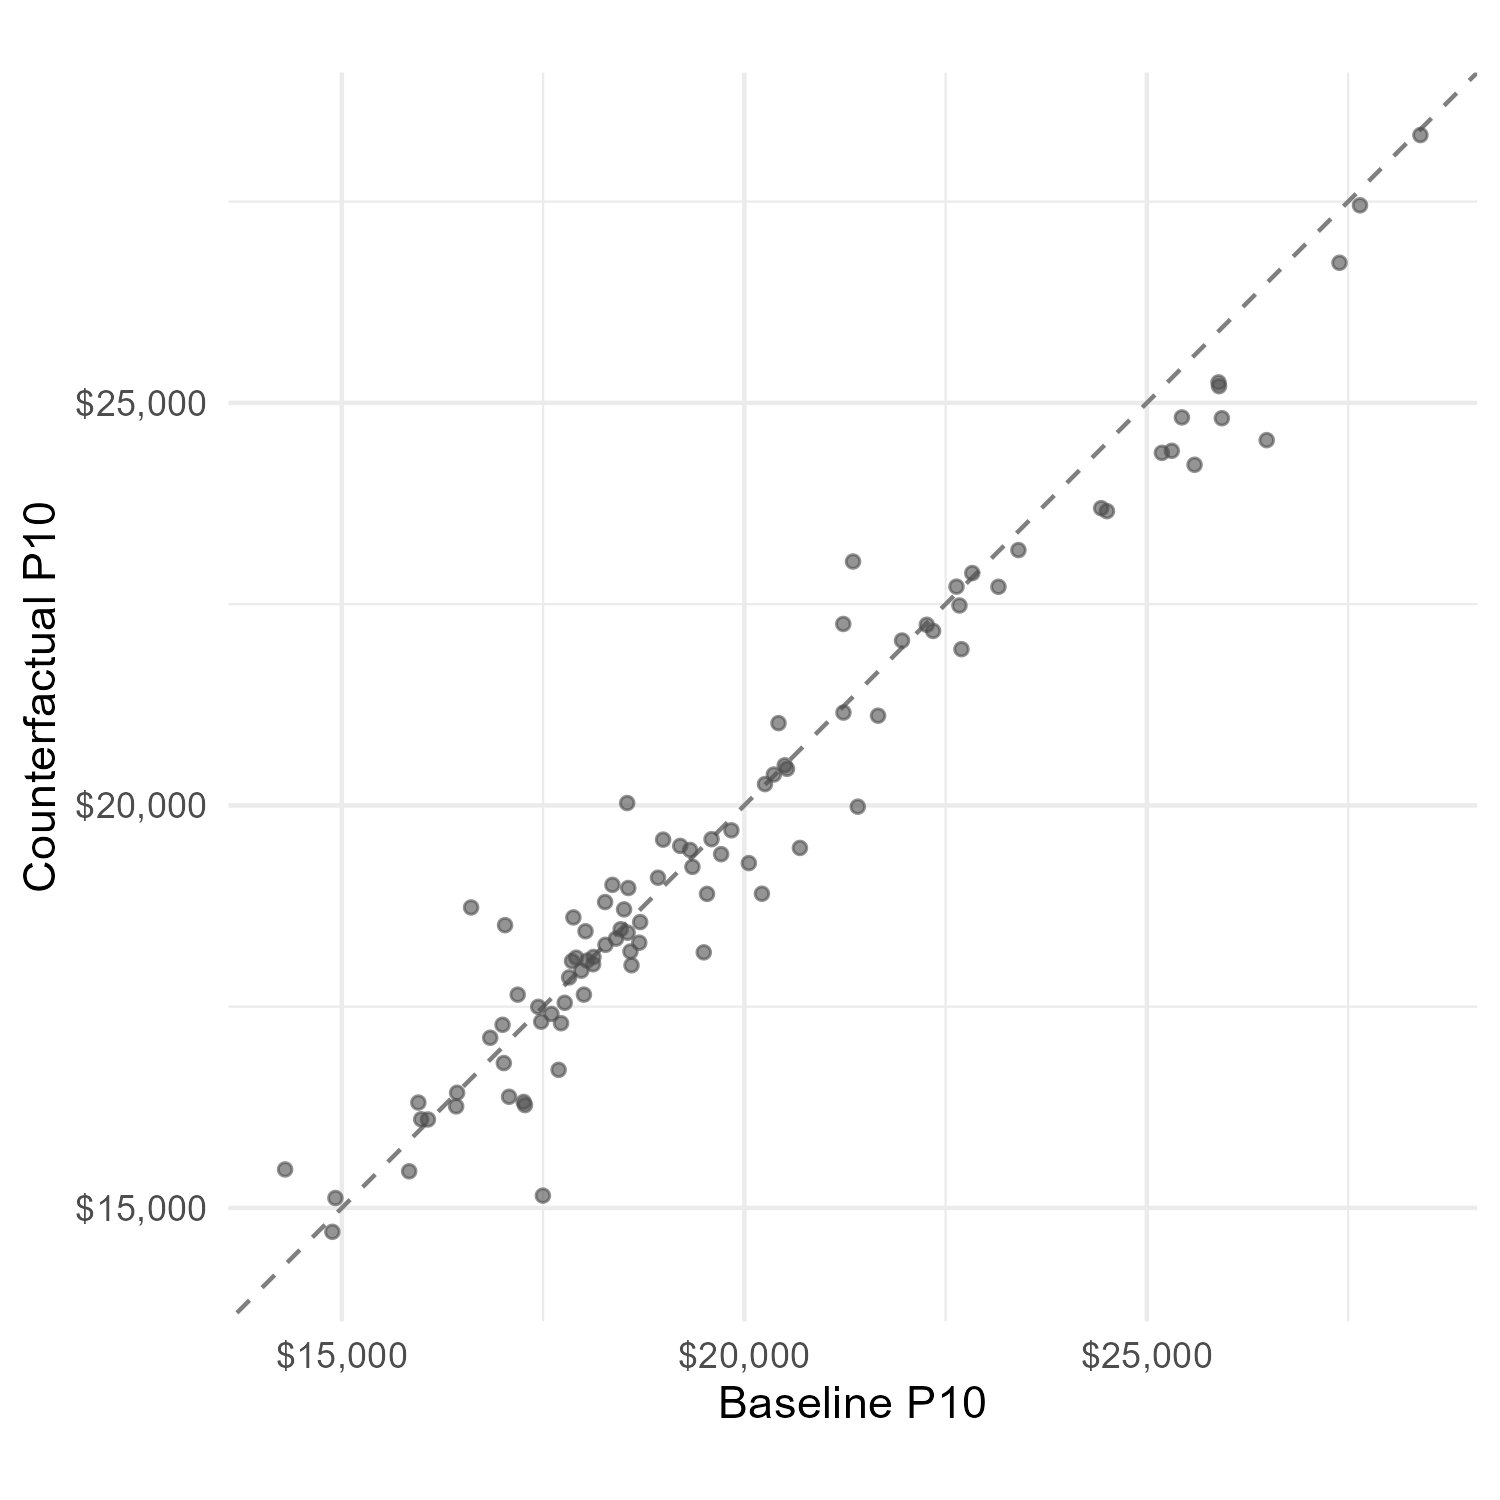
\includegraphics[height=2.2in,width=2.5in,keepaspectratio]{../../../results/figures/myopic-timevary/SpendOffDiag_P10_full_Myopic_eta5.png} \\
\multicolumn{2}{c}{\textit{Forward-looking}} \\
Existing familiarity & Reset familiarity \\
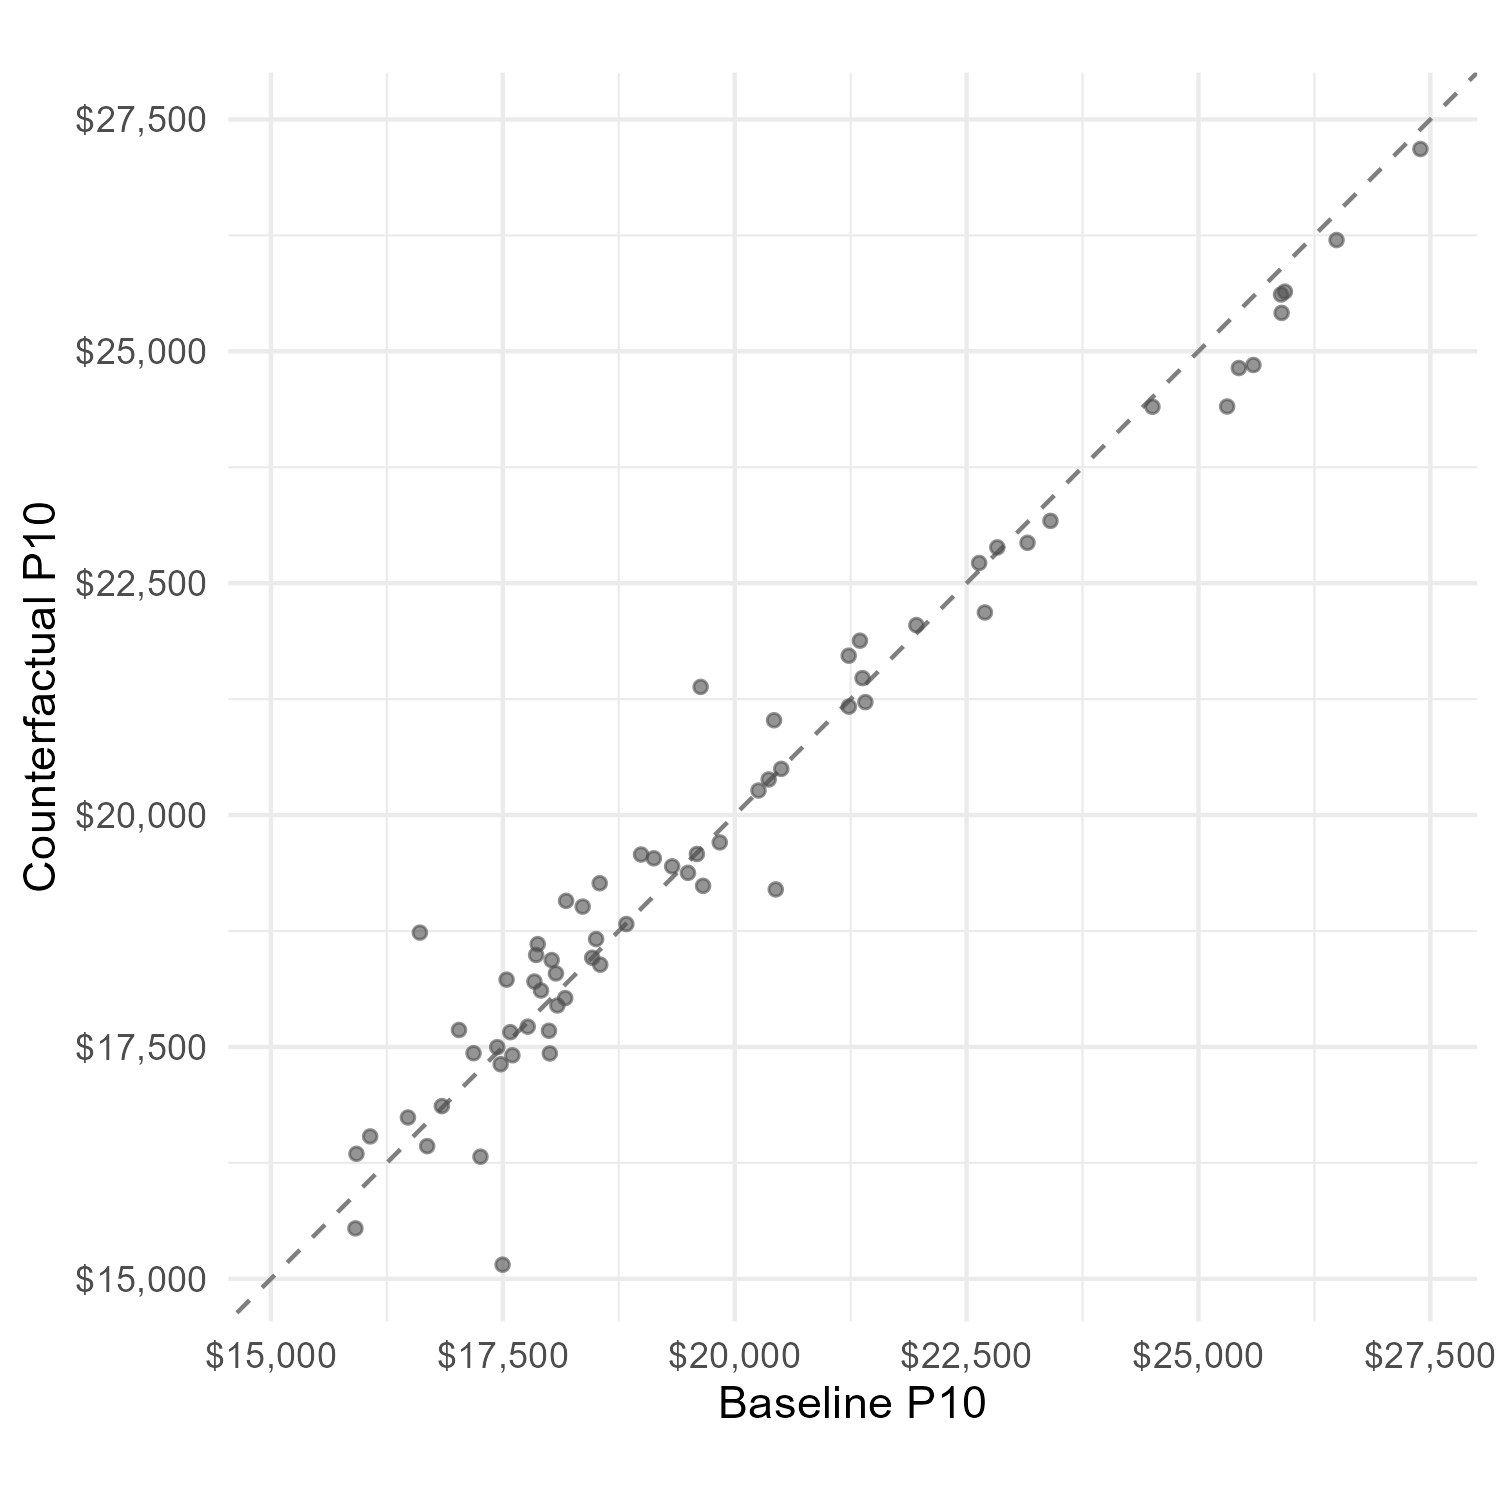
\includegraphics[height=2.2in,width=2.5in,keepaspectratio]{../../../results/figures/fwd-timevary/SpendOffDiag_P10_current_FWD_eta5.png} & 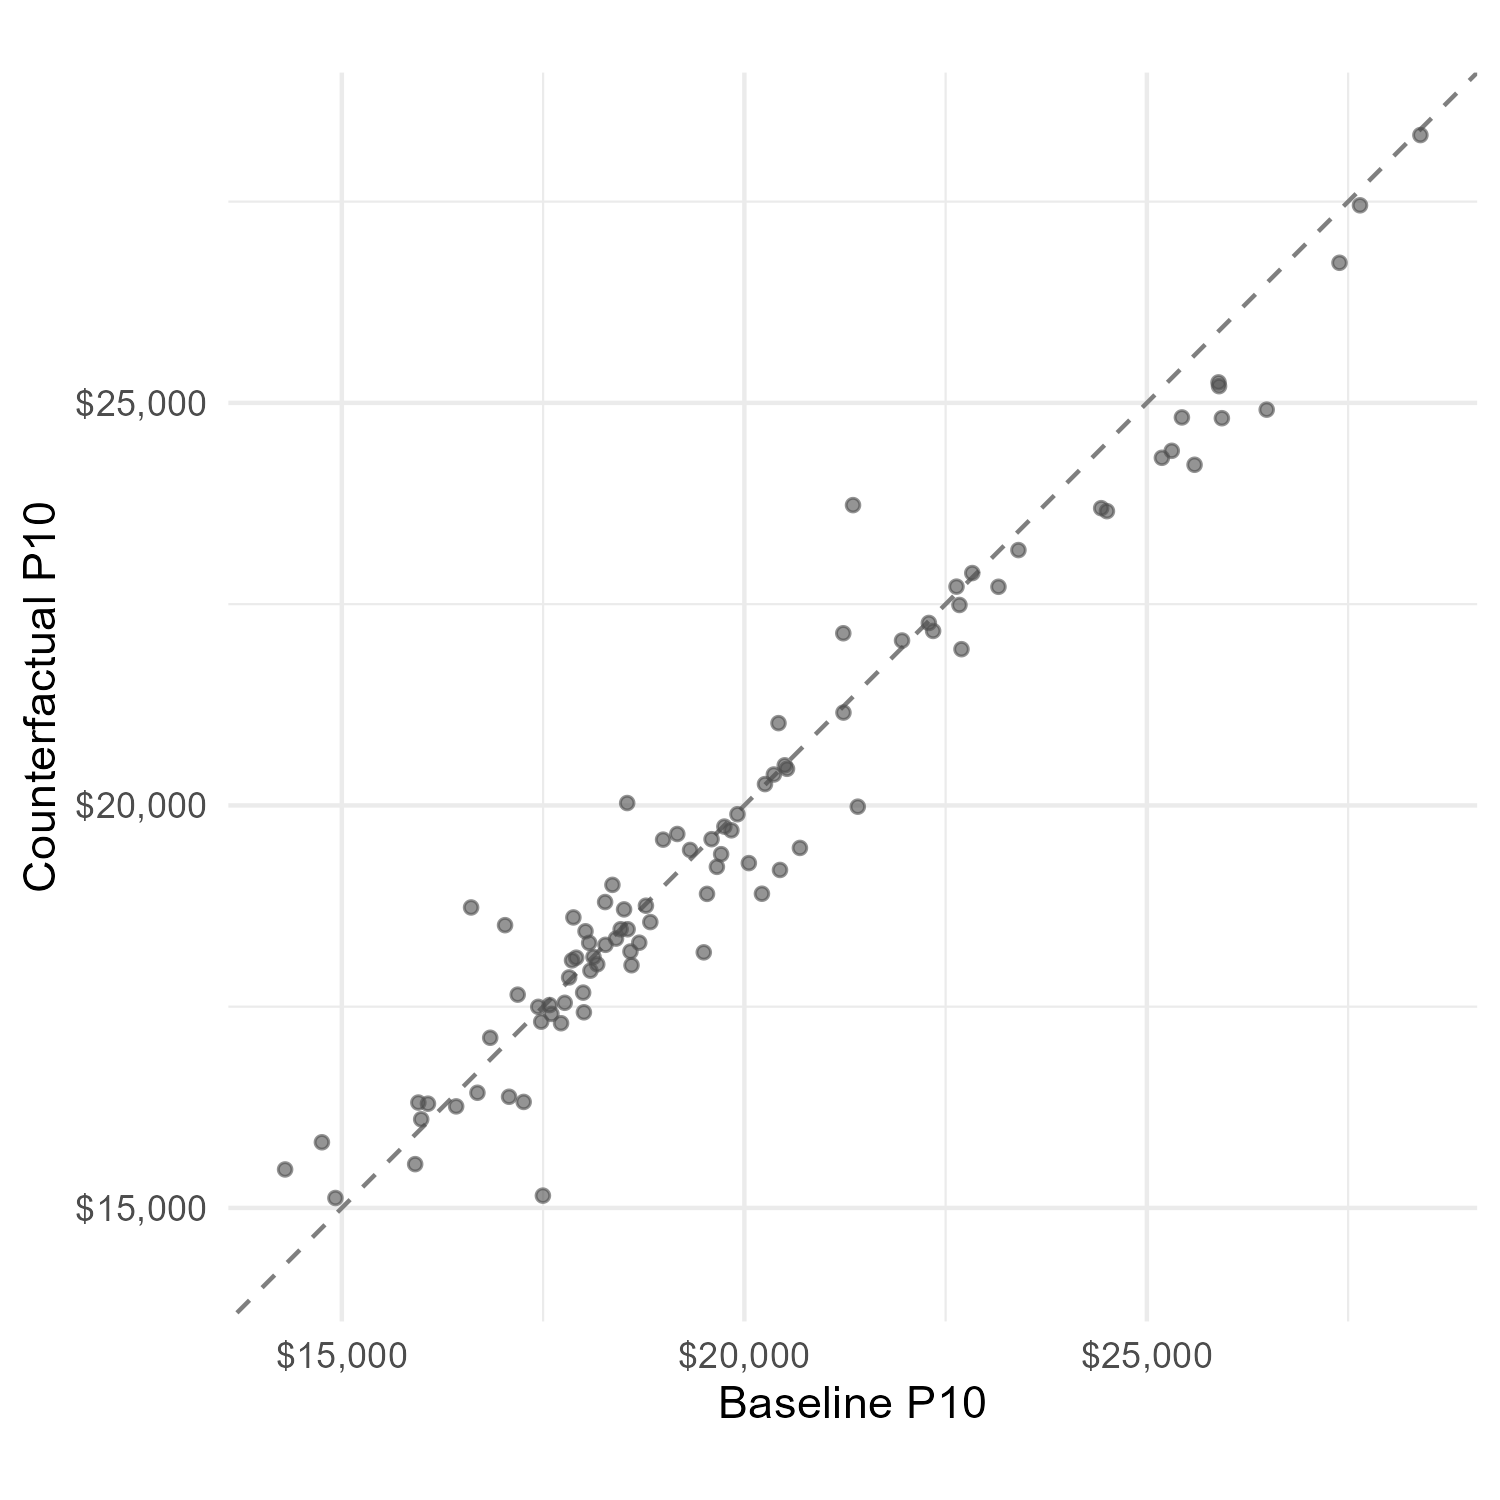
\includegraphics[height=2.2in,width=2.5in,keepaspectratio]{../../../results/figures/fwd-timevary/SpendOffDiag_P10_full_FWD_eta5.png}
\end{tabular}
\label{fig:spendP10-cf-eta5}
\end{minipage}
\end{figure}

\clearpage
\begin{figure}[!ht]
\centering
\begin{minipage}[h]{6in}
\caption[SpendP90 Off-Diagonal ($\eta=5$)]{Off-Diagonal Scatter of Patient-Weighted 90th-Percentile Spending ($\eta=5$)\footnote{Each point is an HRR where the patient-weighted 90th percentile of episode spending under the counterfactual differs from the baseline value. HRRs with identical baseline and counterfactual percentile are dropped (they lie on the 45-degree line). The solid reference line is the 45-degree line.}}
\centering
\begin{tabular}{cc}
\multicolumn{2}{c}{\textit{Myopic}} \\
Existing familiarity & Reset familiarity \\
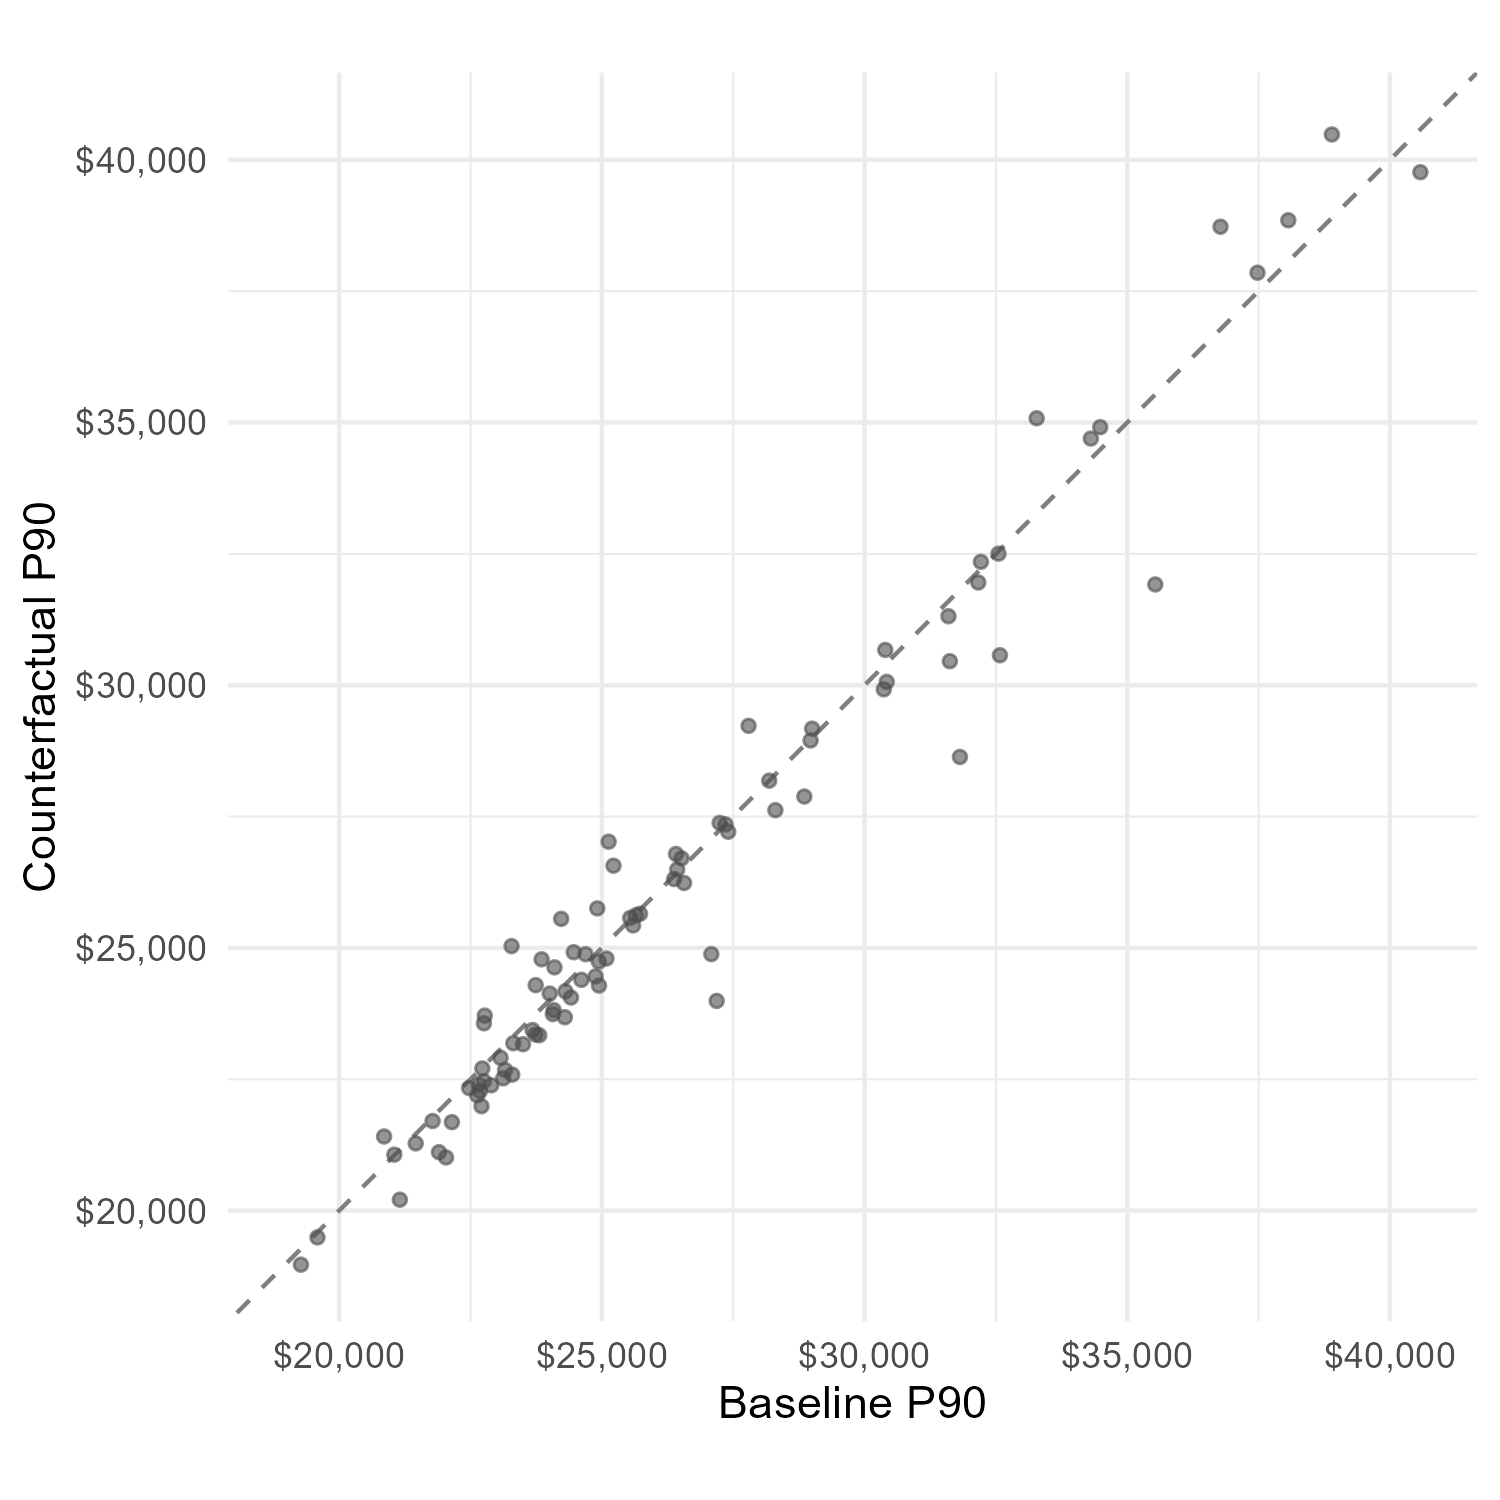
\includegraphics[height=2.2in,width=2.5in,keepaspectratio]{../../../results/figures/myopic-timevary/SpendOffDiag_P90_current_Myopic_eta5.png} & 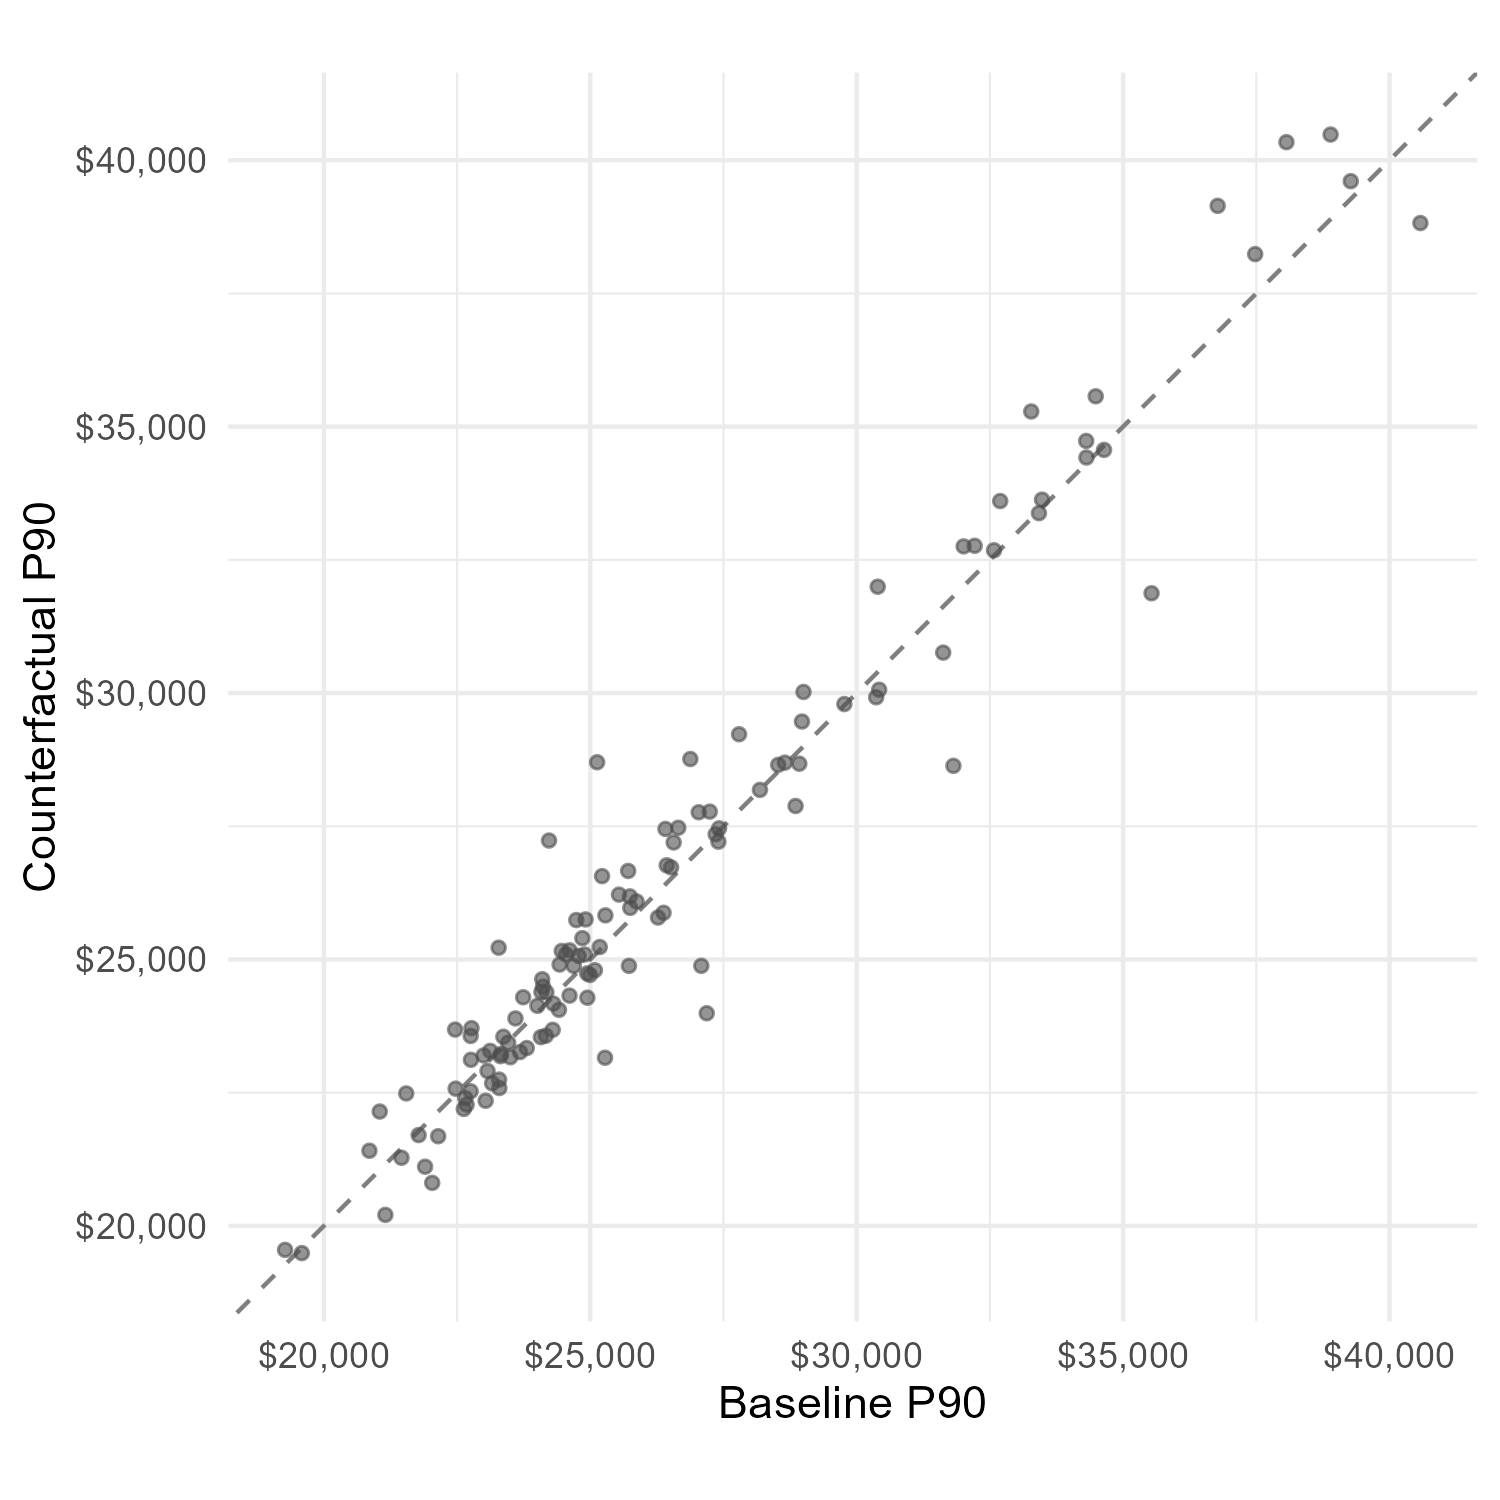
\includegraphics[height=2.2in,width=2.5in,keepaspectratio]{../../../results/figures/myopic-timevary/SpendOffDiag_P90_full_Myopic_eta5.png} \\
\multicolumn{2}{c}{\textit{Forward-looking}} \\
Existing familiarity & Reset familiarity \\
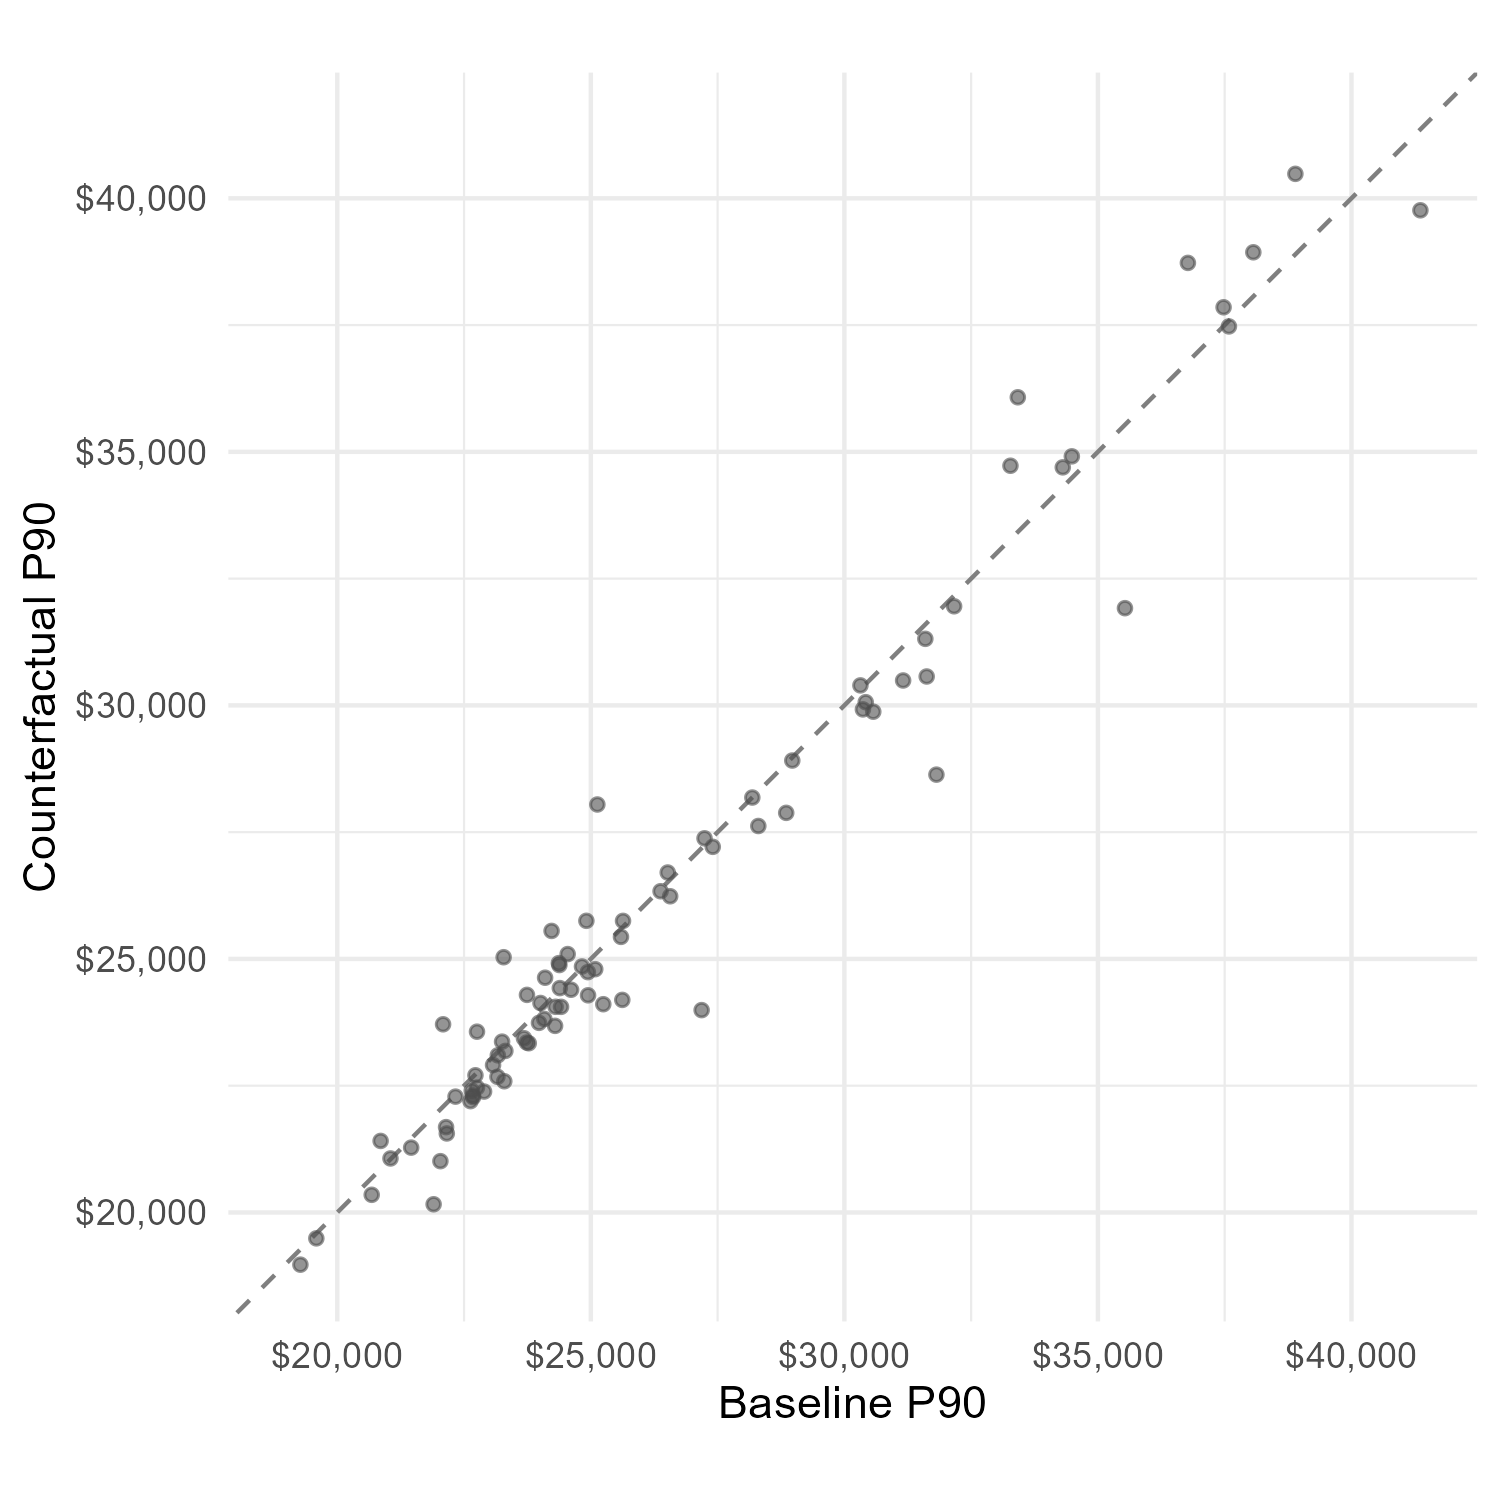
\includegraphics[height=2.2in,width=2.5in,keepaspectratio]{../../../results/figures/fwd-timevary/SpendOffDiag_P90_current_FWD_eta5.png} & 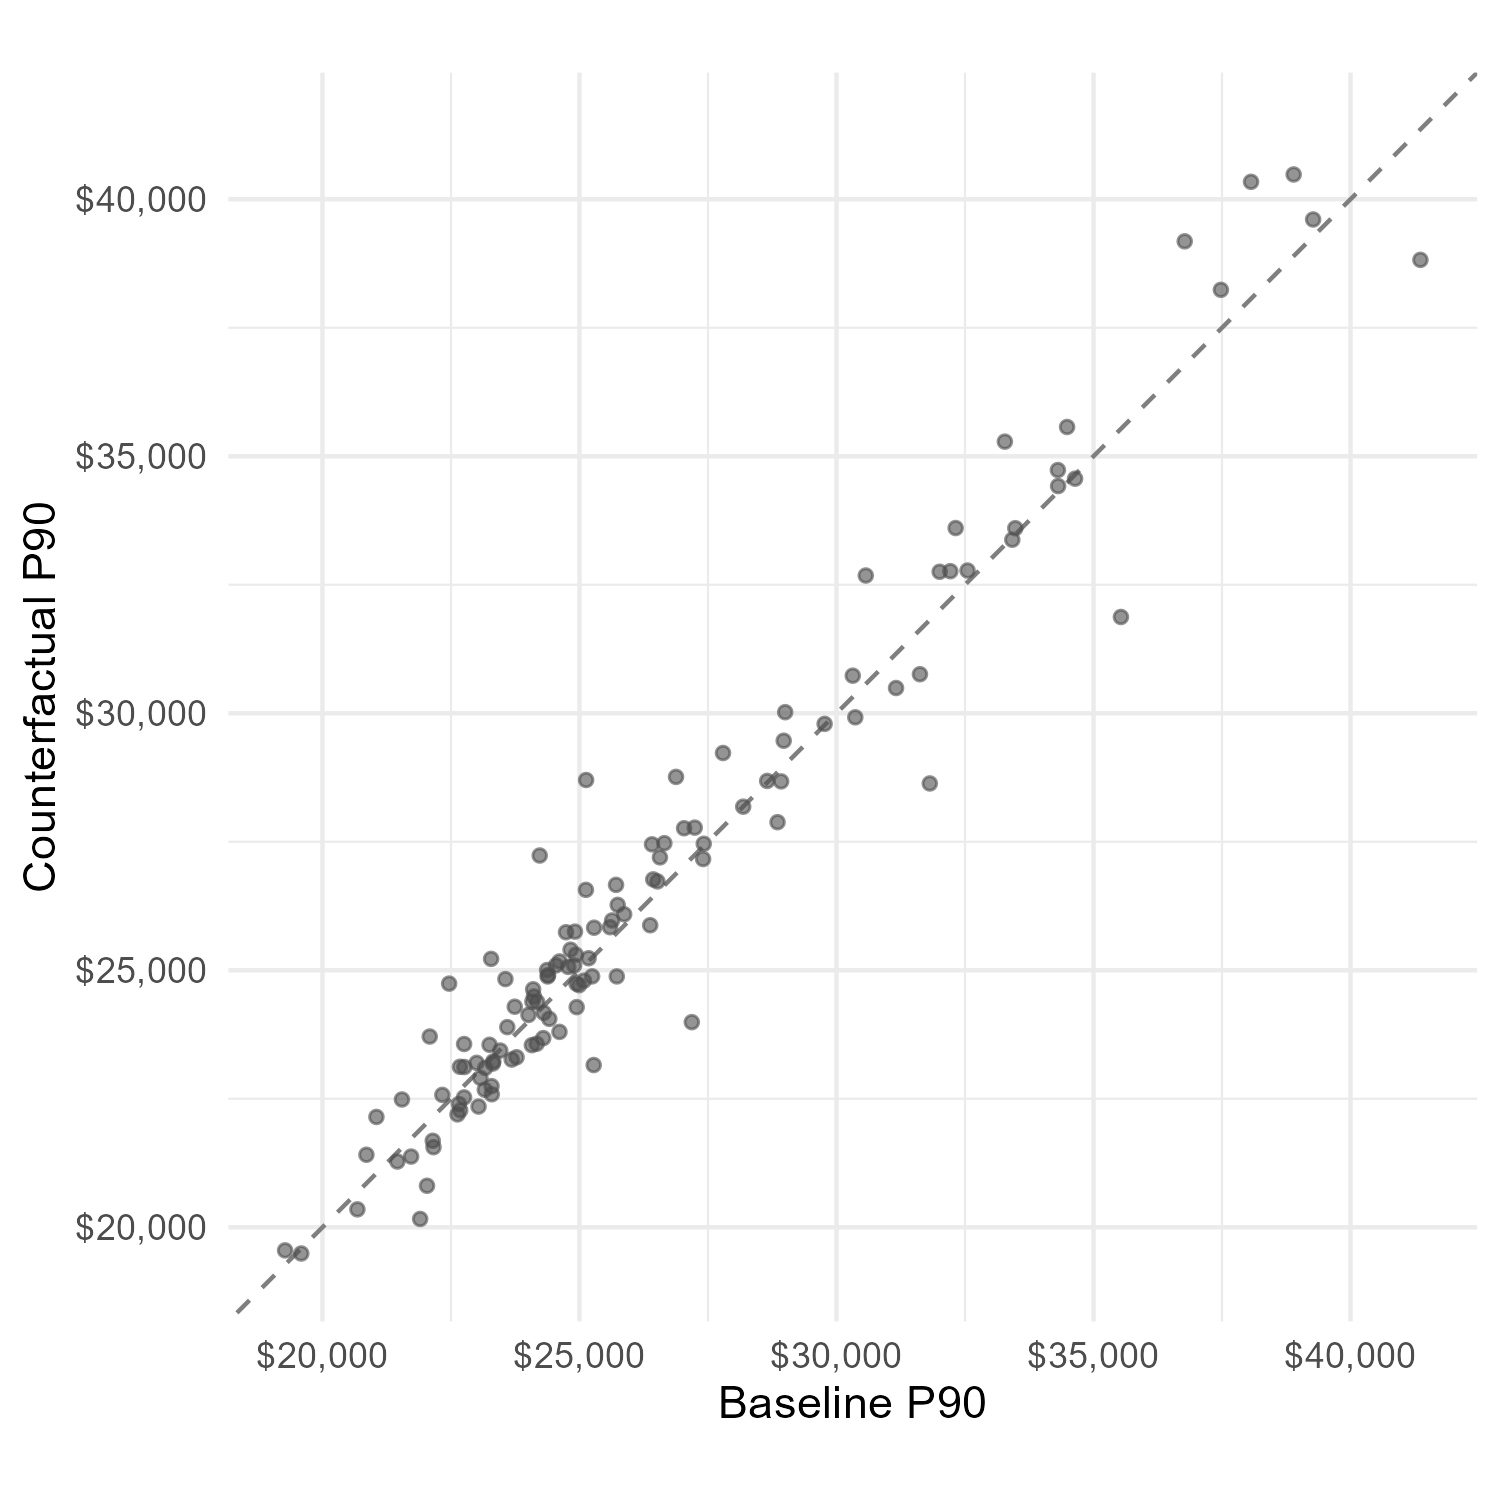
\includegraphics[height=2.2in,width=2.5in,keepaspectratio]{../../../results/figures/fwd-timevary/SpendOffDiag_P90_full_FWD_eta5.png}
\end{tabular}
\label{fig:spendP90-cf-eta5}
\end{minipage}
\end{figure}


\clearpage
\begin{figure}[!ht]
\centering
\begin{minipage}[h]{6in}
\caption[Quality-Maximizing Referrals ($\eta=5$)]{Counterfactual Changes with Quality-Maximizing Referrals ($\eta=5$)\footnote{Figure depicts the share of referrals reallocated and the resulting change in probability of success under a counterfactual in which each PCP's belief is replaced with the true specialist success rate, specialist fixed effects and accumulated familiarity are set to zero, and $\alpha$ within each HRR is calibrated to match the larger of the distance or congestion utility components. Results are averaged across individuals within an HRR and presented as a histogram across HRRs.}}
\centering
\begin{tabular}{cc}
\multicolumn{2}{c}{\textit{Reallocation of referrals}} \\
Myopic & Forward-Looking \\
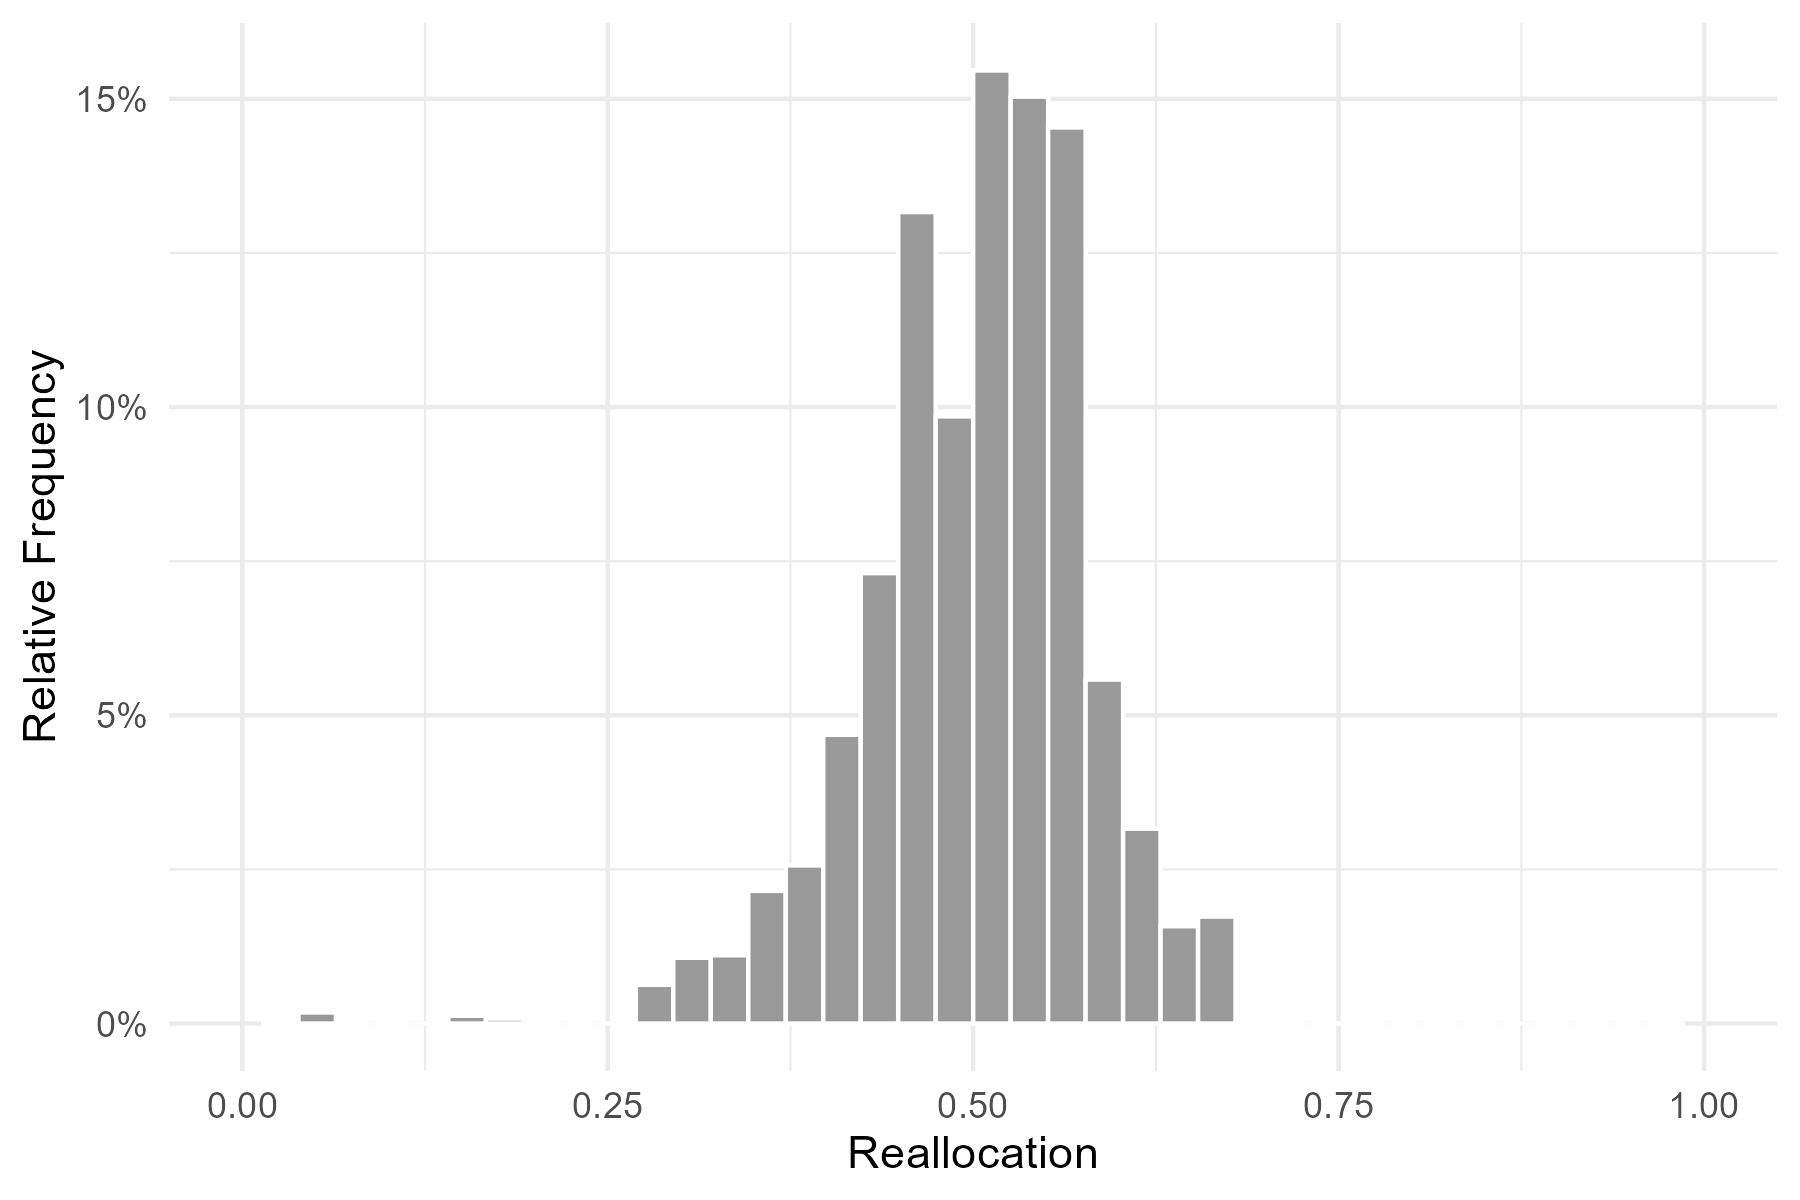
\includegraphics[height=1.8in,width=2.7in,keepaspectratio]{../../../results/figures/myopic-timevary/Reallocation_qualmax_amatch_Myopic_eta5.png} & 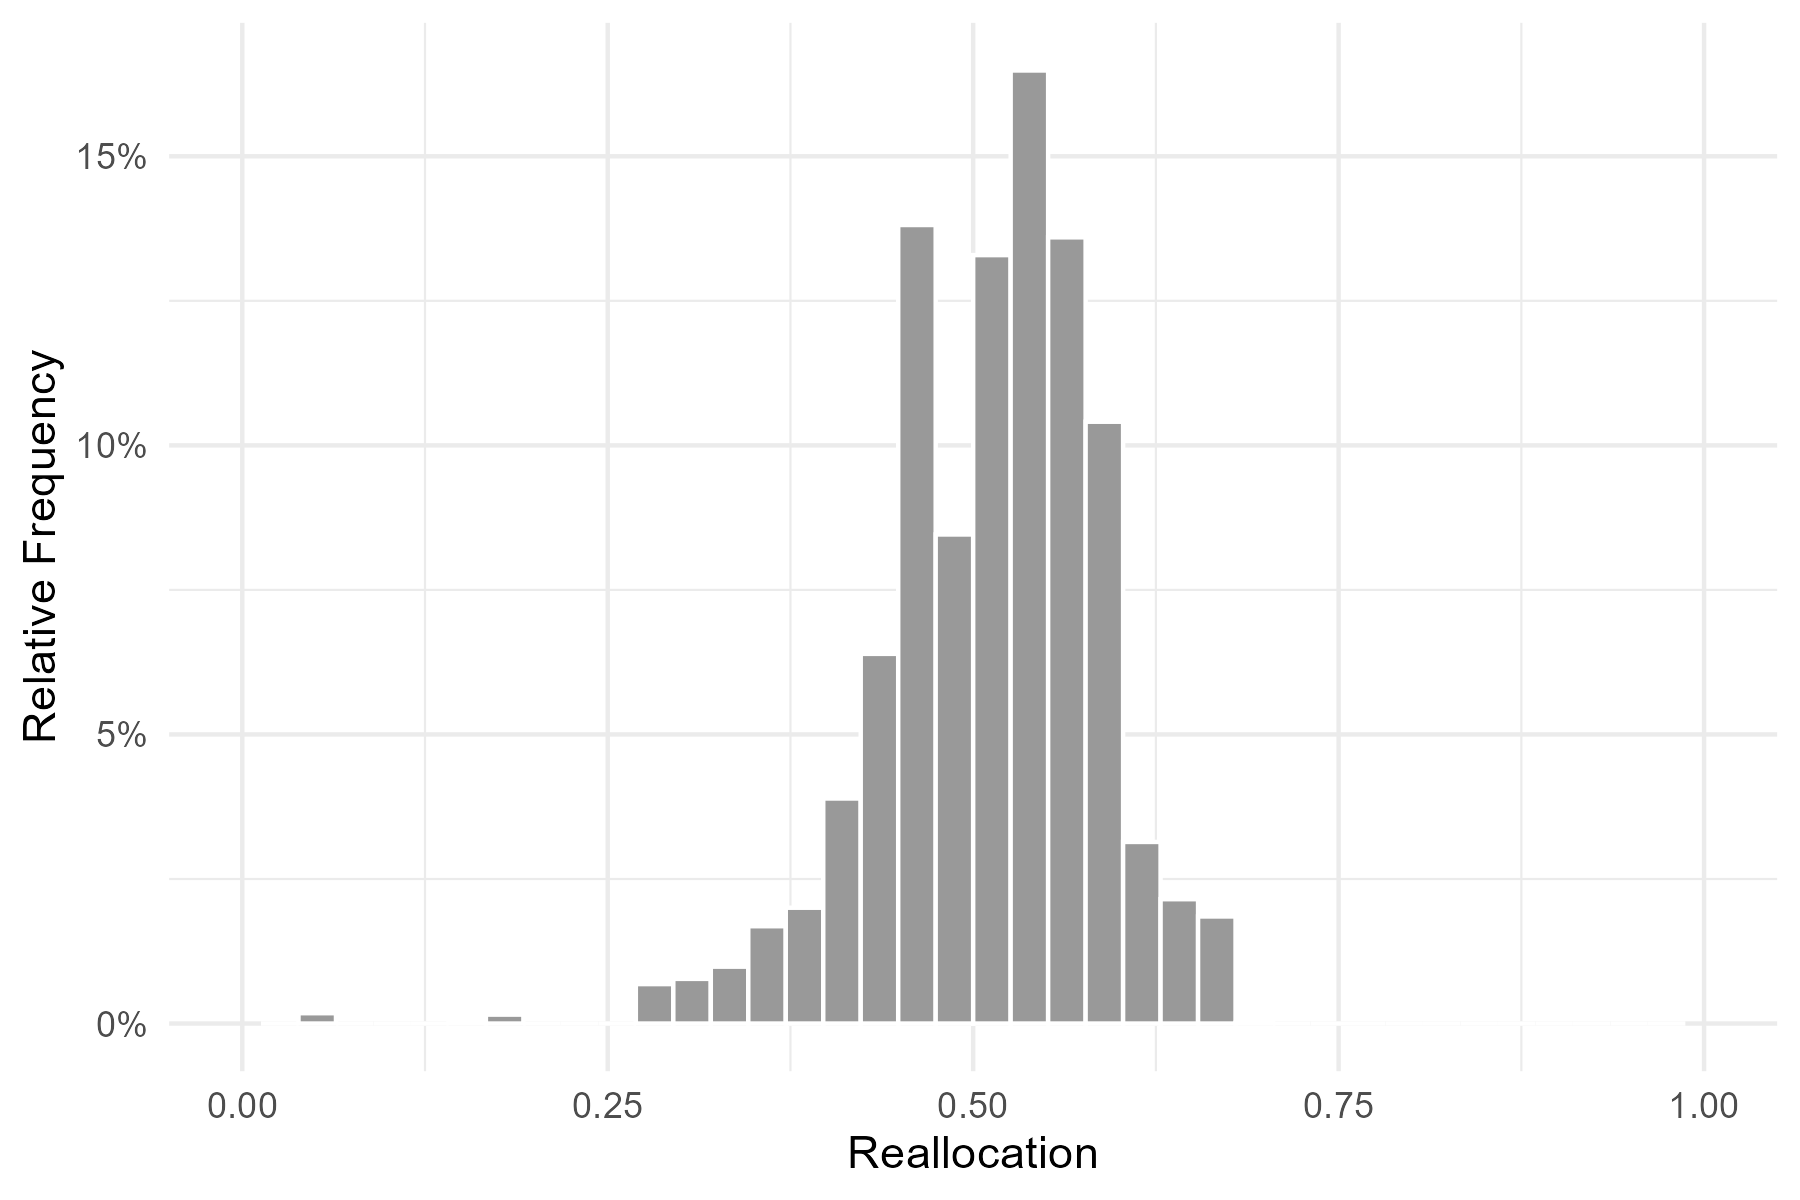
\includegraphics[height=1.8in,width=2.7in,keepaspectratio]{../../../results/figures/fwd-timevary/Reallocation_qualmax_amatch_FWD_eta5.png} \\
\multicolumn{2}{c}{\textit{Change in probability of success}} \\
Myopic & Forward-Looking \\
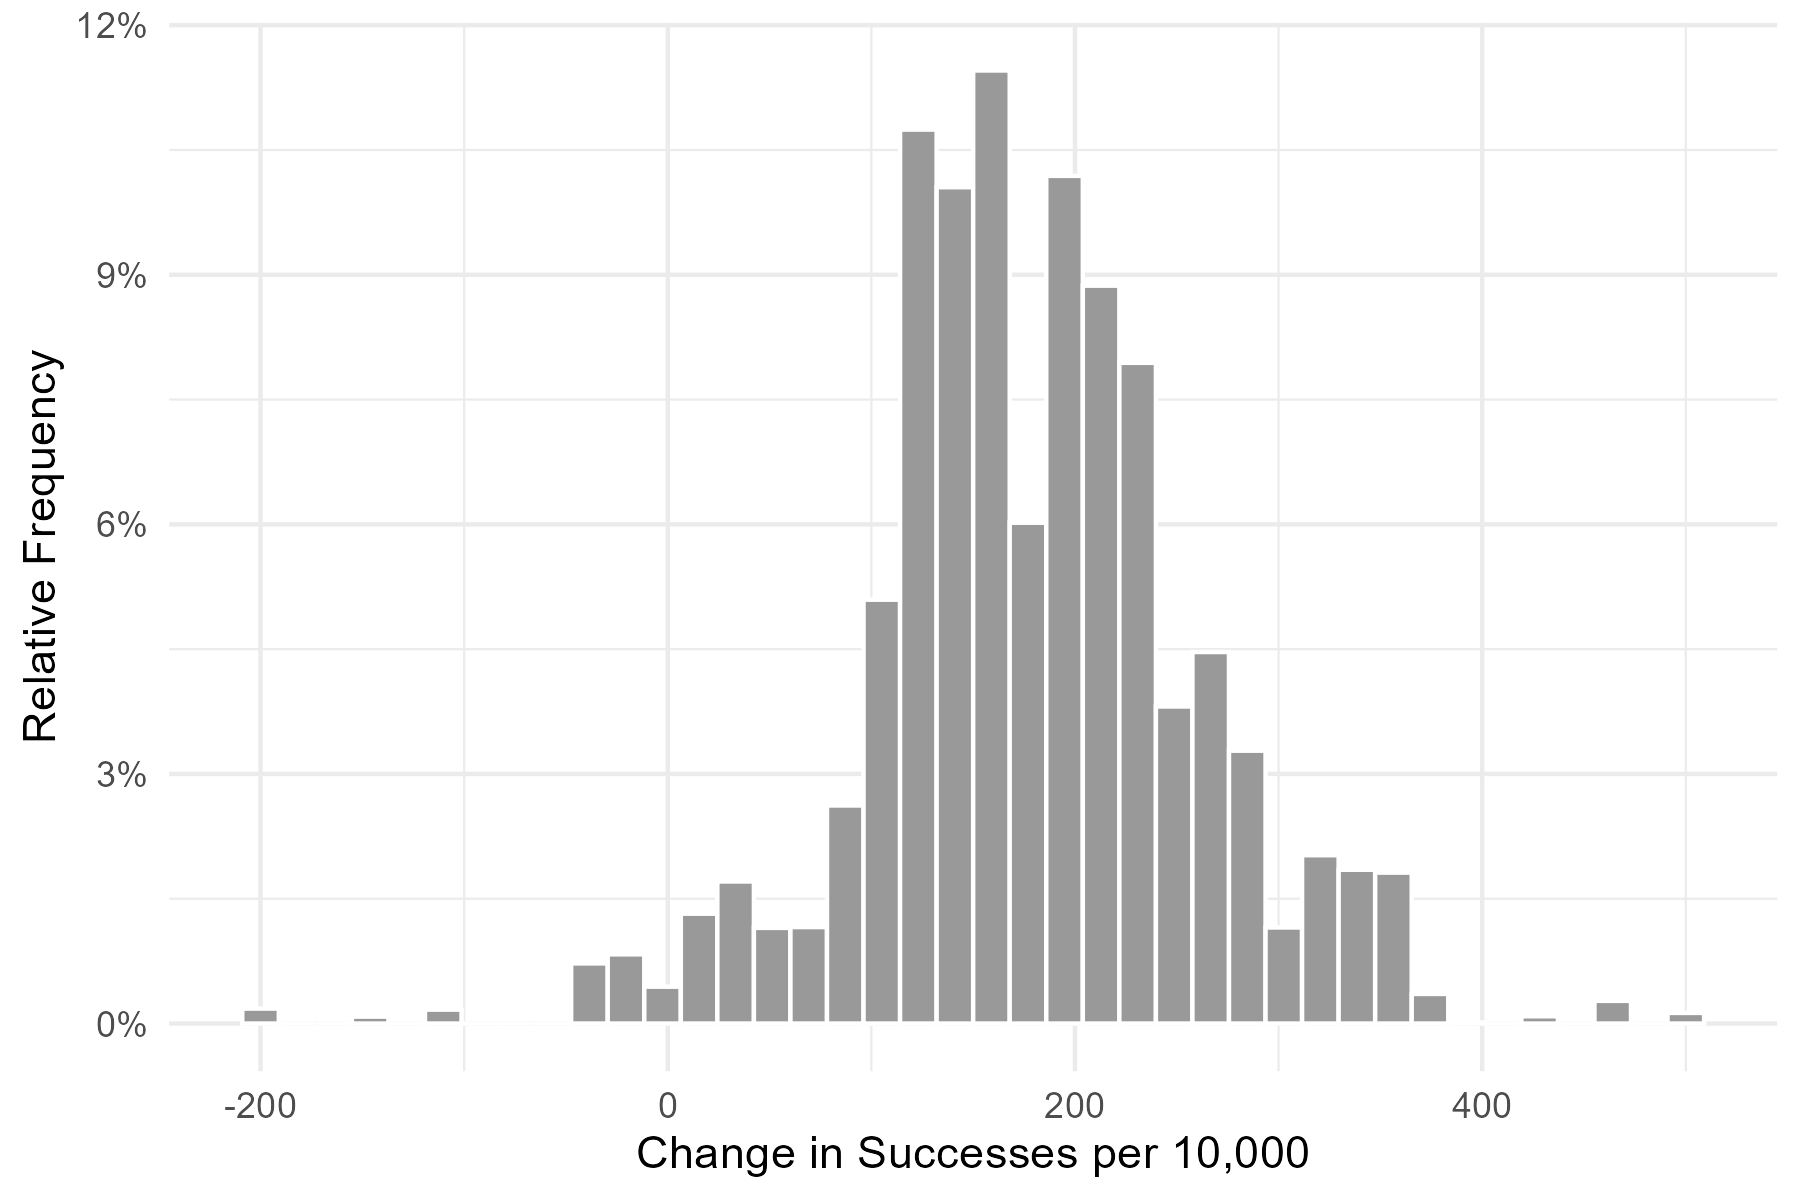
\includegraphics[height=1.8in,width=2.7in,keepaspectratio]{../../../results/figures/myopic-timevary/Mean_Health_FX_qualmax_amatch_Myopic_eta5.png} & 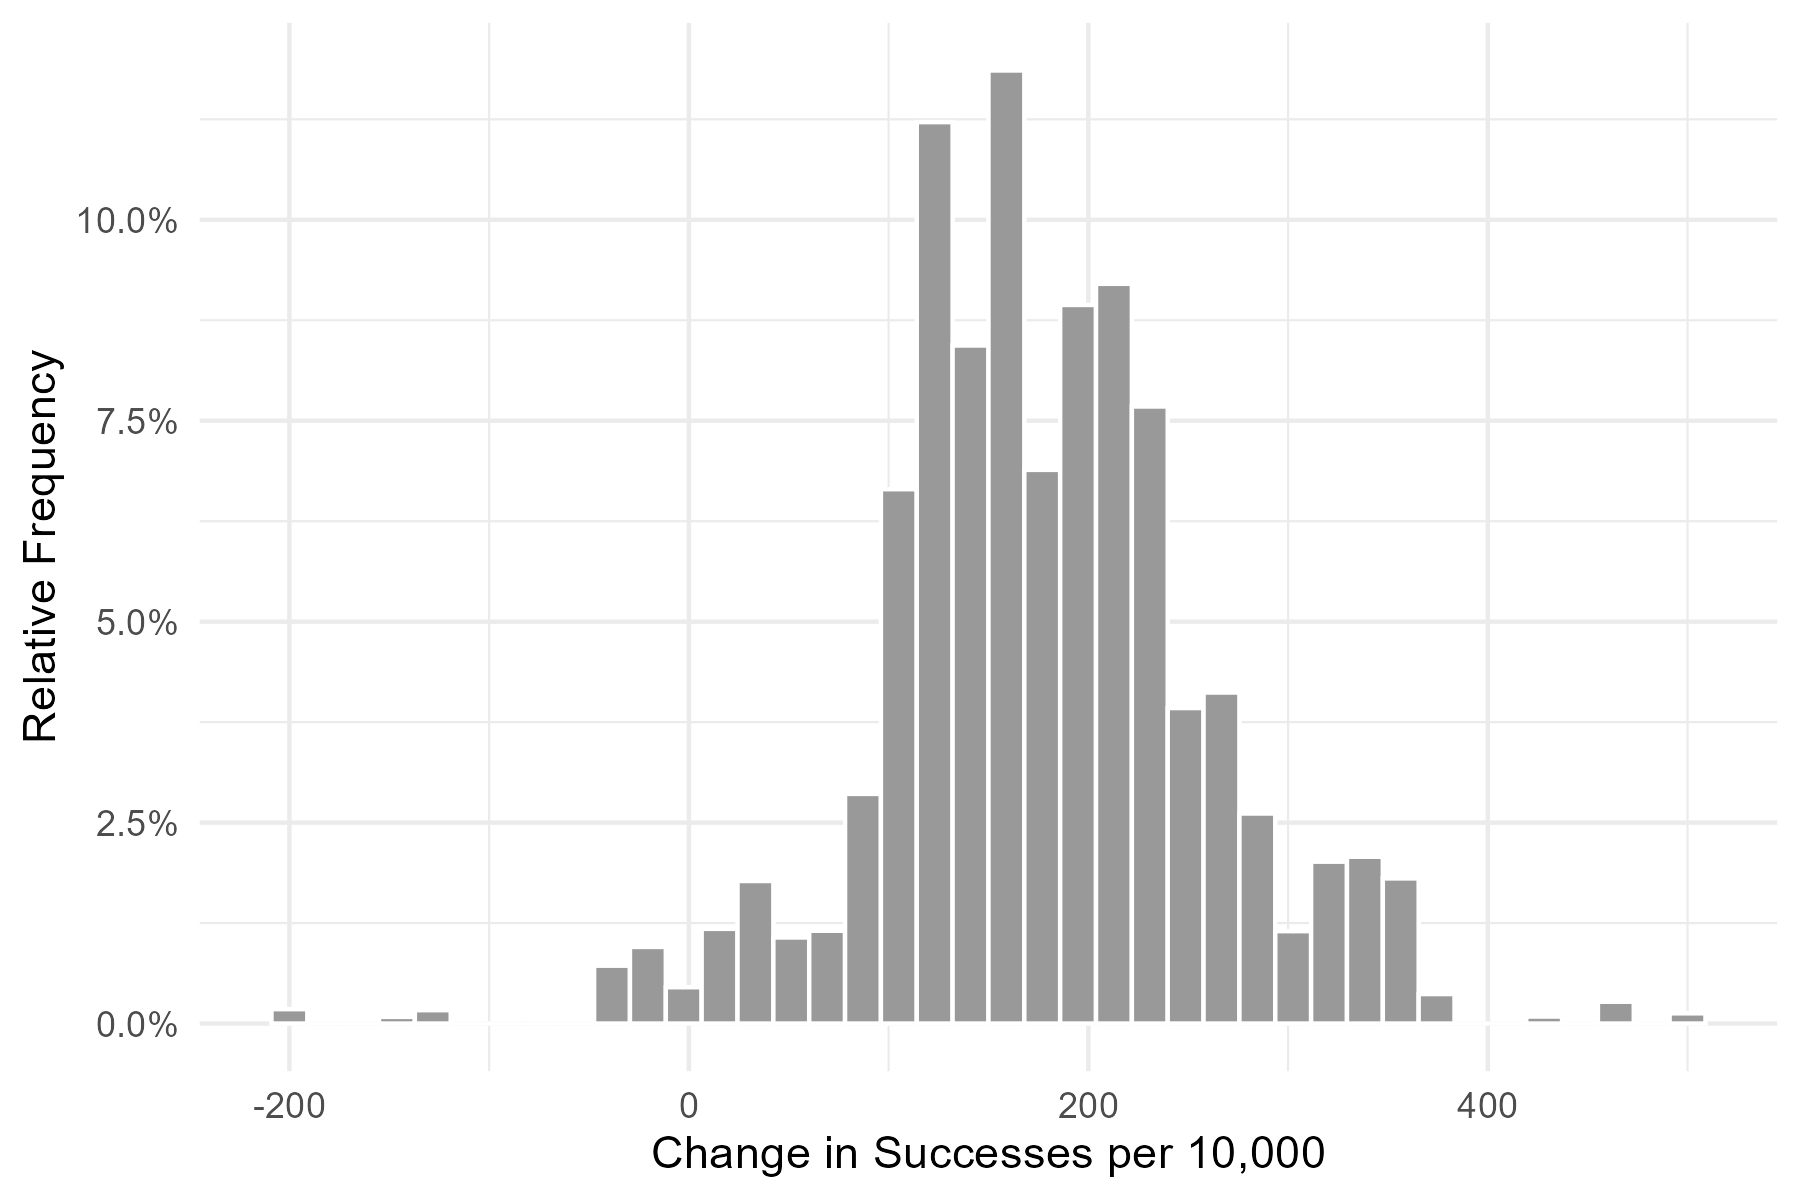
\includegraphics[height=1.8in,width=2.7in,keepaspectratio]{../../../results/figures/fwd-timevary/Mean_Health_FX_qualmax_amatch_FWD_eta5.png}
\end{tabular}
\label{fig:cf_qualmax_eta5}
\end{minipage}
\end{figure}


\end{document}

